\documentclass[12pt]{article}

% USEPACKAGES
\usepackage[table]{xcolor}
\usepackage[margin=2.5cm]{geometry} % Change border margins.
\usepackage[titles]{tocloft} % Table of Contents, manual add.
\usepackage{mcode} % Load matlab code into LaTeX.
\usepackage[parfill]{parskip} % Removes indents
\usepackage[hidelinks]{hyperref} % Clickable links in PDF.
\usepackage{fancyhdr}
\usepackage{graphicx}
\usepackage{epstopdf}
\usepackage{float}
\usepackage{amsmath,amssymb,amsthm,multirow,algorithm,algorithmic,amsfonts}
\usepackage{gensymb}
\usepackage[square,numbers,comma,sort&compress]{natbib}
\usepackage[titletoc]{appendix}
\usepackage[final]{pdfpages}
\usepackage{afterpage}
\usepackage{mdwlist} % Compact lists (itemize*)
\usepackage{fixltx2e}
\usepackage{expl3}
\usepackage{datatool}
\usepackage[nogroupskip,acronyms,symbols]{glossaries}
\usepackage{glossary-longragged}
\usepackage{wrapfig}
\usepackage{caption}
\usepackage{multicol}
\usepackage{subcaption}
\usepackage{pgfplots}

\usepackage{lscape}
\usepackage{rotating}
\usepackage{pdflscape}


\usepackage{pifont}

\usepackage{array}

\newcolumntype{C}[1]{>{\centering\arraybackslash}p{#1}}

%\usepackage{setspace}

\newcommand{\cmark}{\ding{51}}%
\newcommand{\xmark}{\ding{55}}%

\newlength\figureheight 
\newlength\figurewidth
\pgfplotsset{compat=1.3}

% PAGESTYLE
\pagestyle{plain}

% Generate the glossary
	% create a new glossary style for the list of symbols
	% copied (but eddited) from http://www.latex-community.org/forum/viewtopic.php?f=5&t=20797
	\newglossarystyle{listos}{%
	  \glossarystyle{altlongragged4col}
	  \setlength{\glsdescwidth}{0.8\textwidth}
	  % allow line wrap in the description column
	  \renewenvironment{theglossary}%
		    {\begin{longtable}{llp{\glsdescwidth}}}%
		    {\end{longtable}}%
		  \renewcommand{\glsgroupskip}{}% make nothing happen between groups
		  \renewcommand*{\glossaryheader}{%
		  \bfseries Symbol & \bfseries Unit & \bfseries Description \\\endhead}%
		  % No heading between groups:
		  \renewcommand*{\glsgroupheading}[1]{}%
		  % Main (level 0) entries displayed in a row optionally numbered:
		  \renewcommand*{\glossentry}[2]{%
		  \glsentryitem{##1}% Entry number if required
		  \glstarget{##1}{\glossentryname{##1}}% Name
			& \glossentrysymbol{##2}% Unit
			& \glossentrydesc{##2}% Description
			\tabularnewline % end of row
		  }%
		  % Similarly for sub-entries (no sub-entry numbers):
		  \renewcommand*{\subglossentry}[3]{%
		  % ignoring first argument (sub-level)
		  \glstarget{##2}{\glossentryname{##2}}% Name
			& \glossentrysymbol{##2}% Unit
			& \glossentrydesc{##2}% Description
			\tabularnewline % end of row
			}%
			% Nothing between groups:
			\renewcommand*{\glsgroupskip}{}%
			}
	
	% create a new glossary style for the list of constants
		% copied (but eddited) from http://www.latex-community.org/forum/viewtopic.php?f=5&t=20797
		\newglossarystyle{listoc}{%
		  \glossarystyle{altlongragged4col}
		  \setlength{\glsdescwidth}{0.8\textwidth}
		  % allow line wrap in the description column
		  \renewenvironment{theglossary}%
		    {\begin{longtable}{lllp{\glsdescwidth}}}%
		    {\end{longtable}}%
		  \renewcommand{\glsgroupskip}{}% make nothing happen between groups
		  \renewcommand*{\glossaryheader}{%
		  \bfseries Symbol & \bfseries Value & \bfseries Unit & \bfseries Description \\\endhead}%
		  % No heading between groups:
		  \renewcommand*{\glsgroupheading}[1]{}%
		  % Main (level 0) entries displayed in a row optionally numbered:
		  \renewcommand*{\glossentry}[2]{%
		  \glsentryitem{##1}% Entry number if required
		  \glstarget{##1}{\glossentryname{##1}}% Name
			& \glsentryuseri{##2}% Value
			& \glossentrysymbol{##2}% Unit
			& \glossentrydesc{##2}% Description
			\tabularnewline % end of row
		  }%
		  % Similarly for sub-entries (no sub-entry numbers):
		  \renewcommand*{\subglossentry}[3]{%
		  % ignoring first argument (sub-level)
		  \glstarget{##2}{\glossentryname{##2}}% Name
			& \glsentryuseri{##2}% Value
			& \glossentrysymbol{##2}% Unit
			& \glossentrydesc{##2}% Description
			\tabularnewline % end of row
			}%
			% Nothing between groups:
			\renewcommand*{\glsgroupskip}{}%
			}

	
\newglossary*{symbol}{List of Symbols}
\newglossary*{constants}{List of Constants}
\makenoidxglossaries
\setacronymstyle{long-short}
\loadglsentries{./Acronyms}
\newglossaryentry{romanletter}{type=symbol,name={},description={\nopostdesc},sort=a}
\newglossaryentry{greekletter}{type=symbol,name={},description={\nopostdesc},sort=b}
\newglossaryentry{romanletterc}{type=constants,name={},description={\nopostdesc},sort=a}
\newglossaryentry{greekletterc}{type=constants,name={},description={\nopostdesc},sort=b}
\loadglsentries{./Symbols}
\loadglsentries{./Constants}



% COMMANDS
\newcommand{\HRule}{\rule{\linewidth}{0.04cm}}
\renewcommand{\abstractname}{{\Large Summary}}
\renewcommand{\cftsecleader}{\cftdotfill{\cftdotsep}}
\setlength{\parskip}{6pt plus4pt minus2pt}
\setcounter{tocdepth}{2}
% ENVIRONMENTS
\newenvironment{drawing}


\begin{document}
% Titlepage
\begin{titlepage}
\begin{center}

% Upper part of the page
\textsc{\LARGE Delft University of Technology}\\[0.3cm]
\textsc{\Large Design Synthesis Exercise}\\[0.5cm]

% Title
\HRule \\[0.4cm]
{\Large \bfseries Design of a Controllable Inflatable Aeroshell}\\[0.2cm]
{\Huge \bfseries Project plan}\\[0.2cm]
\HRule \\[1.2cm]

% Image
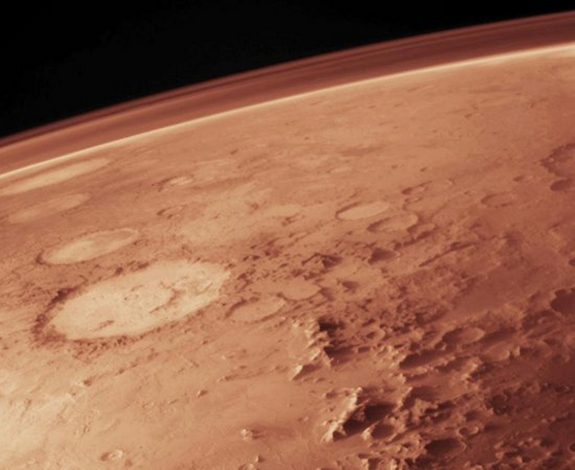
\includegraphics[scale=0.4]{./Titlepage/coverpicture}\\[1cm]

% Author
S. Balasooriyan \\
B. van Dongen \\
D.D. Hage \\
T. Keijzer \\
G. van Koppenhagen \\
L. Mathijssen \\
J. Meulenbeld \\
A. van Oostrum	\\
S. van Schie \\




\vfill

% Date
\begin{large}\today \end{large}

\end{center}
\end{titlepage}
\pagenumbering{roman}

% Summary
\newpage
\section*{Preface}\label{cha:preface}

\begin{flushright}
	\today
\end{flushright}

Dear Reader,	
\\ [1cm]
A growing interest in manned spaceflight and human exploration of Mars requires a new solution. Conventional, rigid entry solutions require a significant decelerator mass to bring the payload to ground. Inflatable concepts offer significant mass and packaging advantages and their application opens up broad venues for interplanetary human spaceflight. 

This Final Report centres around the analysis and design of a \acrlong{cia} that is capable of bringing two crew members to the Martian surface with a mere $10\%$ decelerator mass fraction within 10 days. Conceptual and preliminary design have shown the feasibility of such a mission with its corresponding economical benefits and reduced ecological footprint by a decreased required number of launches through increased payload-carrying capability.

We would like to acknowledge dr. ir. H.J. Damveld, ir. D. Dolkens and ir. N. Reurings for their guidance and support. Moreover, we would like to thank all other staff members of the Delft University of Technology that have been of assistance.
%This Mid-Term Report is part of the deliverables for the \acrfull{mtr}. It describes the development, verification and validation of the computational tools produced to analyse several possible concepts for a controllable inflatable aeroshell designed for manned spaceflight. In addition to analysing these concepts a trade-off will be made between them to determine which is the most promising. This concept will then be further analysed in the coming period. The goal of this project is to develop an inflatable aeroshell system that can be used for atmospheric entry on Mars and is lighter than the current solutions to this problem.
\\ [1.5cm]
Design Synthesis Exercise Group 02

\section*{Summary}\label{cha:summary}


Inflatable aeroshell concepts hold the key to what is currently unattainable for interplanetary human spaceflight. In the wake of current \acrfull{nasa} investigations on the feasibility of inflatable decelerators for hypersonic guidable re-entry, this study focuses on Mars entry of a payload mass of at least 9000 [kg] using an inflatable aerodynamic decelerator of at most 1000 [kg]. Such a solution provides a large economical advantage over conventional solutions by maximizing payload-carrying capability through a light-weight device less burdened by launcher size considerations. This Mid-term Report gives an overview of conceptual design activities, comprising aerodynamic, structural, thermal, astrodynamic and control tool development and analysis, leading up to concept selection in a trade-off.
\newline
\newline
To aid in the conceptual analysis, design and selection process and to provide a basis for further design efforts after concept selection in the \acrfull{mtr} a number of tools have been developed with the following purposes:
\begin{itemize}
\item A tool for parametric structural mass modelling
\item A modified Newtonian flow aerodynamic tool for the characterisation of aerodynamic and aerothermal behaviour
\item A thermal model for \acrfull{tps} sizing and analysis
\item An astrodynamic tool with an implemented control system for trajectory control
\end{itemize}

Concepts were selected for trade-off as the outcome of a structured \acrfull{dot} on the basis of concept shape. Shape is chosen to have a leading factor due to its importance in the aerodynamic and trajectory performance, which directly flows down to thermal, structural and control performance. The initial concept selection yielded five concepts for trade-off: a conventional capsule concept and four inflatable concepts, namely stacked toroid, tension cone, trailing ballute and isotensoid configurations. To reflect concept capability of meeting customer demand, the following concept aspects have been evaluated as trade-off criteria: decelerator mass, development risk, vehicle stability and deceleration time.
\newline
\newline
The first trade-off criterion, decelerator mass, is essential since it is highly desirable that payload-carrying capability is maximised. To make full use of the launcher carrying capability, a decrease in decelerator mass allows for an equal increase in payload mass. To this end, structural, thermal and control system mass were estimated as the distinguishing mass components between concepts. 

The lowest structural mass was achieved by the stacked toroid configuration, followed upon closely by the isotensoid, tension cone and trailing ballute configurations (an estimated 110, 168 and 221 \% of stacked toroid structural mass respectively). \acrfull{tps} and control system mass analysis yielded estimates of 100, 84, and 76 \% and 100, 67, and 96 \% of stacked toroid mass for tension cone, trailing ballute and isotensoid configurations respectively. This yields total decelerator masses of 116, 113 and 88 \% of stacked toroid mass, based on weight contributions of 20, 50 and 15 \% by structure, \gls{tps} and control system mass. A mass analysis for the rigid concept showed a decelerator mass well in excess of the imposed maximum 1000 [kg], 2945 [kg] for thermal and structural mass alone.
\newline
\newline
The second trade-off criterion, development risk, is essential since concepts with a low \acrfull{trl} incur higher schedule and cost risks. The tried-and-true rigid solution thereby has \gls{trl} 9, while inflatable concepts are notably less explored. A recent surge in interest in inflatable concepts by \gls{nasa} and a consistent development program has brought the stacked toroid configuration to \gls{trl} 7. The other three inflatable concepts are less explored, having only undergone a selected set of tests and research and hence designated \gls{trl} 4. The trailing ballute concept is deemed to have a higher development risk still, by its only feasible control option being a relatively underdeveloped one, namely morphing, reflected by \gls{trl} 2.
\newline
\newline
The third trade-off criterion, deceleration time, is evaluated as a shorter entry time is desirable. As ground operations are to be maintained at fully capacity during entry, a shortening of entry time will alleviate costs incurred. Moreover, physical taxation of human payload is decreased as deceleration time is decreased.  A decreased deceleration time is obtained by better controlability of the spacecraft. To this end, concepts were evaluated for their performance in lift to drag ratio. The rigid concept was found to be able to provide a relatively high lift to drag ratio which consequently will result in short deceleration time. The stacked toroid, tension cone and ballute concept were found to provide an adequate value and finally the isotensoid deceleration performance was found to be poor in this trade-off criteria.
\newline
\newline
It is preferable that concepts are stable, since a stable vehicle will counteract perturbations to move back to its equilibrium condition and its intended trajectory. To this end, static stability was investigated by aerodynamic analysis. Stacked toroid, tension cone and ballute were found to be stable; the rigid concept is neutrally stable and the isotensoid is unstable. The first three therefore perform well, the rigid concept performs adequately and performance of the isotensoid is deficient for the fourth and final trade-off criterion.
\newline
\newline
On the basis of the analysis presented in this Mid-Term Report, design options and their prospective advantages and disadvantages are presented to the customer at the \gls{mtr}. Hereafter dialogue is entered to yield a final concept for preliminary design that satisfies customer demands. The next phase then commences with a more detailed analysis and design of the selected concepts, aided by tool enhancement. This phase entails a more refined orbit optimization, aerodynamic shape determination and structural and \gls{tps} design and sizing. A structured approach to this next phase is facilitated by breaking down future work, resource allocation and is aided by an interface definition given in this report to define the interaction of subsystems within the design process.


% Table of contents
\newpage
\tableofcontents
\addtocontents{toc}{\protect\contentsline {section}{Acronyms}{v}{}}
\addtocontents{toc}{\protect\contentsline {section}{List of symbols}{vi}{}}
\addtocontents{toc}{\protect\contentsline {section}{List of Figures}{vii}{}}
\addtocontents{toc}{\protect\contentsline {section}{List of Tables}{viii}{}}

\newpage
\printnoidxglossary[type=\acronymtype,nonumberlist]
\newpage
\renewcommand{\arraystretch}{1.1}
\printnoidxglossary[type=symbol,nonumberlist,style=listos]
\printnoidxglossary[type=constants,style=listoc]
\newpage
\listoffigures
\newpage
\listoftables

% Chapters
\newpage
\pagenumbering{arabic}

\section{Introduction}
\label{cha:introduction}
Before human interplanetary spaceflight can be achieved technological gains have to be made in several fields. One of these fields comprises hypersonic deceleration systems. Significant weight gains are expected to be possible by using inflatable aeroshells. However, the development of a controllable inflatable aeroshell is very complex and consists of many different disciplines. To reduce the complexity of designing such a system first a \acrfull{pp} was made. Following that a \acrfull{br} was produced, in order to survey the current technology state and knowledge on this subject. Now a \acrfull{mtr} report is made in order to perform a concept trade-off. 

The purpose of this report is to present several concepts for a controllable inflatable aeroshell and to determine which concept is best suited for performing the design mission. First the group organisation for the period between the \acrlong{mtr} and \acrlong{fr} is discussed in chapter \ref{ch:wdd}, including individual and group tasks and work packages. A \acrfull{wbs} is made, together with a \acrfull{wfd} and Gantt chart. Secondly the approach with respect to sustainable development is presented in chapter \ref{ch:sustain}. Thirdly the \glspl{dot} are used in chapter \ref{ch:options} to generate several system concepts. These concepts will be analysed with tools from several different disciplines. These consist of an astrodynamics \& control tool, as well as tools for concept mass estimation, aerodynamical characteristics and thermodynamic behaviour. The development, verification, validation of these tools is discussed in chapters \ref{ch:astrocontrol}, \ref{ch:strucmass}, \ref{ch:aero_analysis} and \ref{ch:thermtool} respectively. These chapters also show the results obtained from analysing the proposed system concepts. After the tool development and concept analysis the risk inherent to each system concept is considered in chapter \ref{ch:riskestimation}. This will be done by making a risk map for each concept. Finally the concept trade-off will be performed in chapter \ref{ch:tradeoff}, based on results of the analyses conducted in the previous chapters. The result of this is a complete trade-off matrix, after which the customer will be able to select the preferred concept based on the weights they attach to each trade-off criterion.
\section{Operational segment}\label{cha:opseg}
This chapter describes the mission operational segment, giving an overview of mission phases and related activities. It serves to identify the actions to be performed by the system over the mission duration. It is essential that these are taken into account in mission design for a complete and feasible mission. To this end, the mission is divided into four phases: 
\begin{itemize}
\item[I]{Interplanetary flight up to the sphere of influence}
\item[II]{Re-entry from the sphere of influence to the point of atmospheric entry}
\item[III]{Re-entry from the point of atmospheric entry to the terminal point at 10 kilometers altitude}
\item[IV]{Final descent from the terminal point at 10 kilometers altitude to ground level}
\end{itemize}
These four phases are discussed hereafter in sections \ref{sec:p1}-\ref{sec:p4}.

\subsection{Phase I}\label{sec:p1}
The first phase imposes the following requirements on the vehicle:
\begin{itemize}
\item The payload shall provide sufficient volume and adequate living capability for human payload. Since the mission strictly only concerns the re-entry part, the relevance of this mission phase is mainly to impose human payload requirements. 
\item  The mission requires use of a launcher. The launcher limits the maximum diameter of the re-entry vehicle as well as its mass, since it is more economically feasible to adhere to current launcher availabilities rather than to develop a new launcher.
\end{itemize}
Moreover, transfer time should be within the limits of human payload endurance. As such, a Hohmann transfer is not a feasible option due to its large transfer time and a higher energy transfer orbit is more realistic. This affects how Mars is approached.

\subsection{Phase II}\label{sec:p2}
The start of the second mission phase signifies the initiation of control system activities in trajectory control.

\subsection{Phase III}\label{sec:p3}

\subsection{Phase IV}\label{sec:p4}
The final descent phase employs deployment mechanisms other than the inflatable aeroshell and demands a high precision in landing at a designated landing site. To this end, the terminal conditions with which the third phase is exited affect the final descent. To avoid requirements on aerodynamic braking in the final descent phase from being overly demanding, from this phase the requirement flows down that at the terminal altitude of 10 [km] the terminal Mach number shall not exceed 5 [-]. 


\section{Work definition and division}
\label{ch:wdd}
This chapter provides an overview of the work involved in the development of an controllable inflatable guidable aeroshell and the allocation of human resources to the defined work. It is essential that planning is adhered to in order to fulfill customer requirements within the allotted timeframe of ten weeks in total with the available resources, namely a team consisting of nine students. 

To this end a \gls{wbs} and \gls{wfd} are presented that categorise and sequence the work activities involved in the project in section \ref{sec:work}. Secondly, managerial and technical functions are appointed to team members in section \ref{sec:org}. Thirdly, the allocation of human resources in time is presented in the form of a Gantt chart in section \ref{sec:gantt}.

\subsection{Work definition}
\label{sec:work}
Work activities are recognized and categorized as depicted in Figure  \ref{fig:wbs}. The \gls{wbs} presented distinguishes conceptual design from preliminary design, where the former is conducted on five concepts and the latter on the concept selected in the trade-off made during the \acrfull{mtr}. This report details the activities taken up to the point of the trade-off, primarily the steps of development and implementation of tools and the analysis of concepts through analysis with the developed tools. Conceptual concept analysis and design takes place on a high level and is centered around the performance of the selected concepts in terms of the trade-off criteria. Preliminary analysis and design proceeds in more detail. Therefore tools are required that allow a more detailed analysis and design, captured by the work activities of tool set expansion. While it is preferable to have a more detailed analysis and design of all selected concepts, the allocated timeframe is a limiting factor. To maximize work efficiency within this timeframe, it is essential that a good planning is made and adhered to. This planning is discussed in section \ref{sec:gantt}.

The \gls{wfd}, presented in Figure  \ref{fig:wfd}, sequences the work activities defined. Primary goal of the \gls{wfd} is to depict how work activities interact. This serves for a time-constrained resource allocation and to identify iteration loops.


\subsection{Technical and managerial team organisation}
\label{sec:org}
Technical functions, as appointed in the \acrfull{pp} \cite{Balasooriyan2015}, have been maintained up to the \gls{mtr} and will be maintained hereafter. This is based on the reasoning that members have gained knowledge and experience of their respective appointed fields to such an extent that their primary responsibility should lie therein. All team members are involved in each field, however, by active communication and interaction during start-of-day, end-of-day and status meetings. The departments are: structural, aerodynamics, trajectory $\&$ control systems and thermodynamics. They are depicted in Figure  \ref{fig:obs}. Department descriptions have been taken up in Appendix \ref{app:obs}

Organisational functions are depicted in Figure  \ref{fig:obs}. The organisational functions will be re-divided amongst team members after the \gls{mtr}, in order to fully explore the capabilities of and to provide the best possible learning experience for all team members. The function descriptions have been taken up in Appendix \ref{app:obs}.

\begin{figure}[H]
\centering
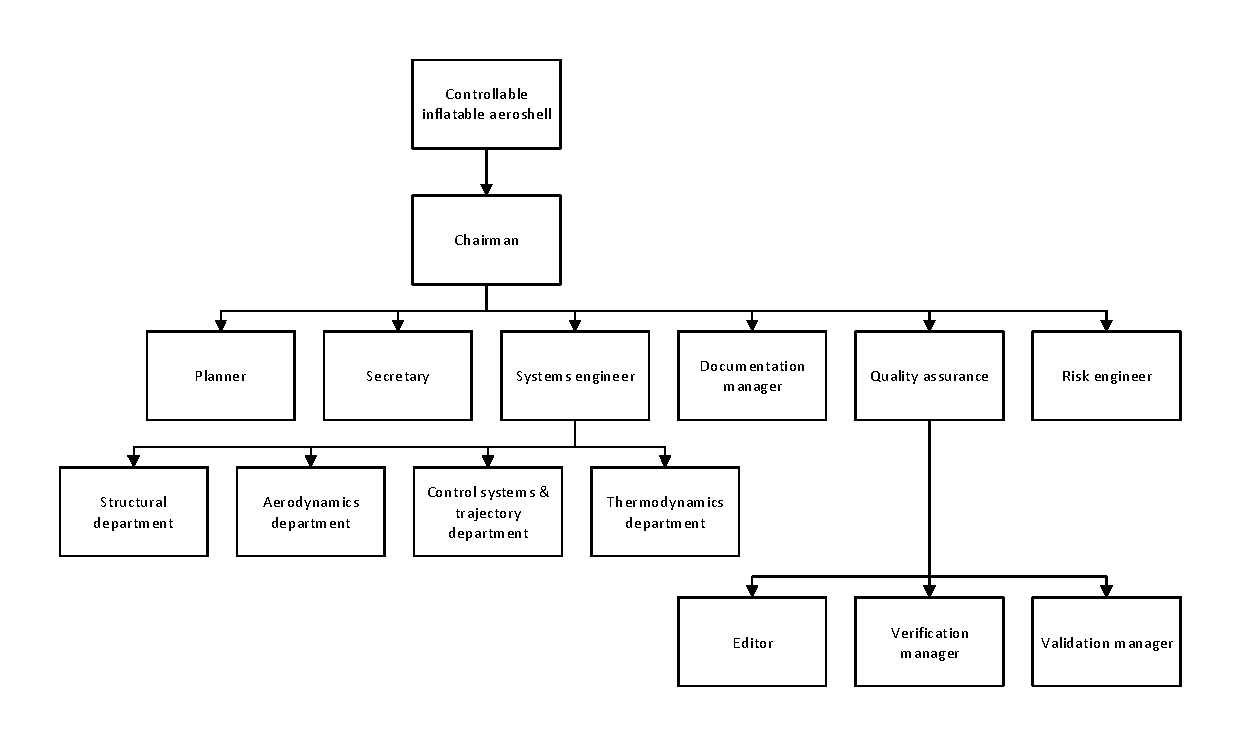
\includegraphics[width=0.95\textwidth]{./Figure/OBS_MTR.pdf}
\caption{Organisational breakdown structure} \label{fig:OBS}
\label{fig:obs}
\end{figure}

\subsection{Human resource allocation}
\label{sec:gantt}
The work activities have been defined in the \gls{wbs} displayed in Figure  \ref{fig:wbs} and sequenced in the \gls{wfd} in Figure  \ref{fig:wfd}. Human resources are allocated to these activities in the Gantt chart, presented in Appendix \ref{app:gantt}. The planner ensures that all team members work according to the deadlines defined in the Gantt chart. Actions taken in case of deadline exceedance are dependent on the nature of the delay.


\begin{sidewaysfigure}[ht]
    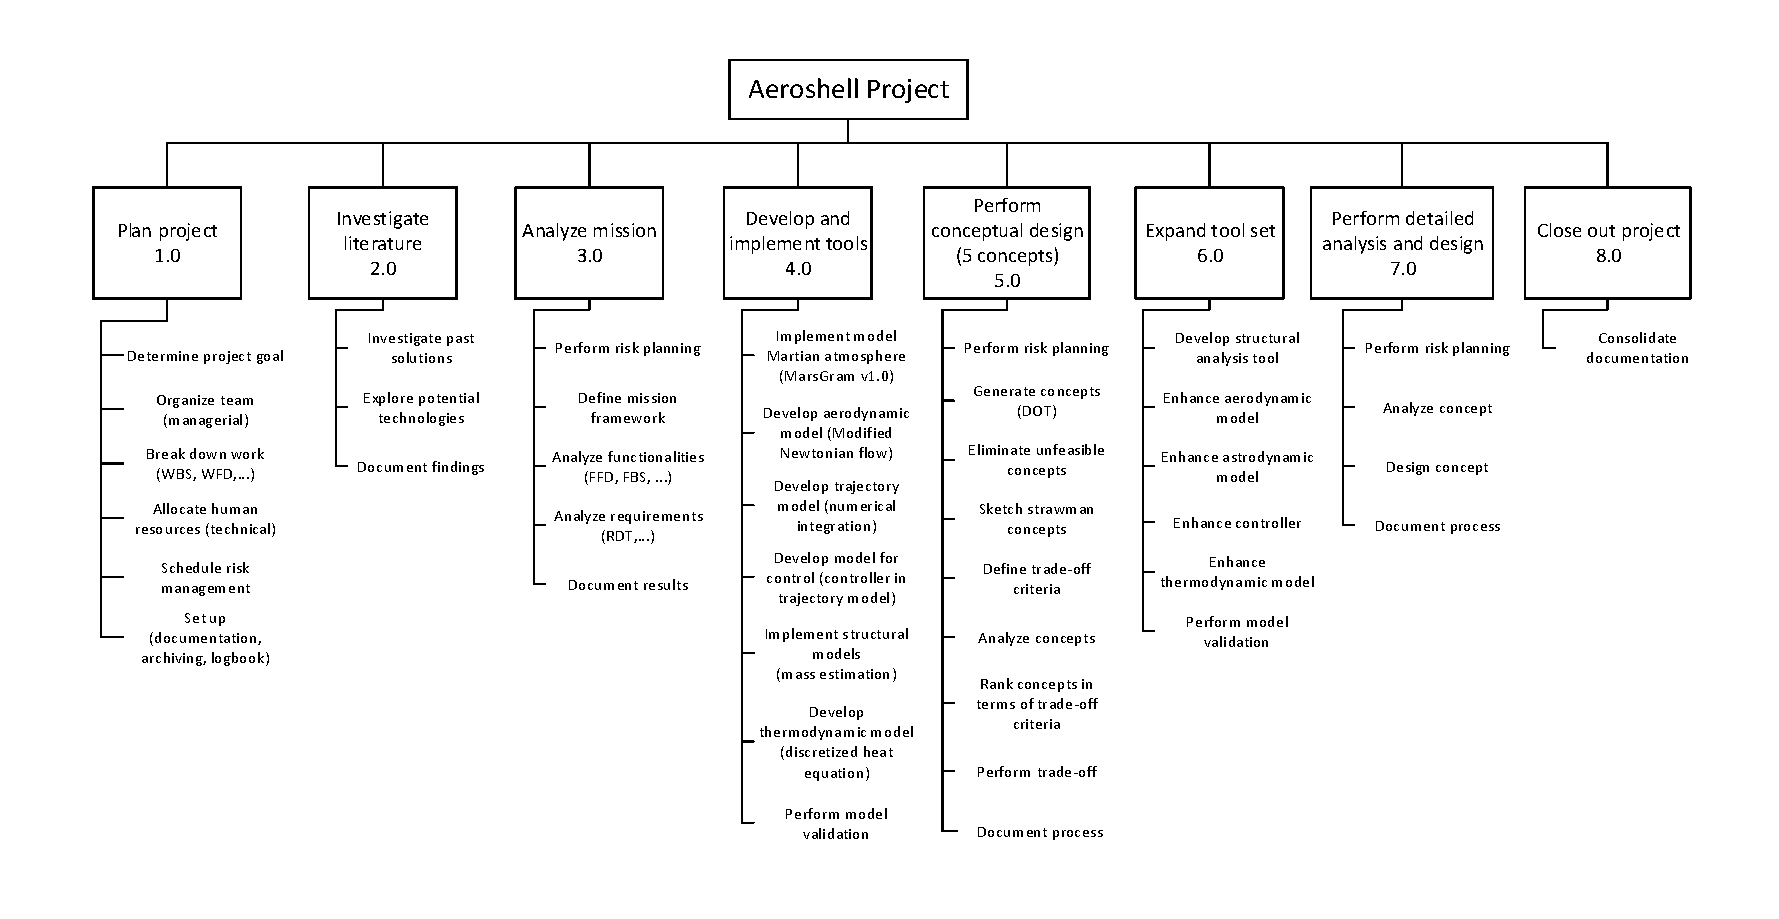
\includegraphics[scale=0.85]{Figure/WBS_MTR.pdf}
    \caption{\acrfull{wbs} of project}
    \label{fig:wbs}
\end{sidewaysfigure}
\begin{sidewaysfigure}[ht]
    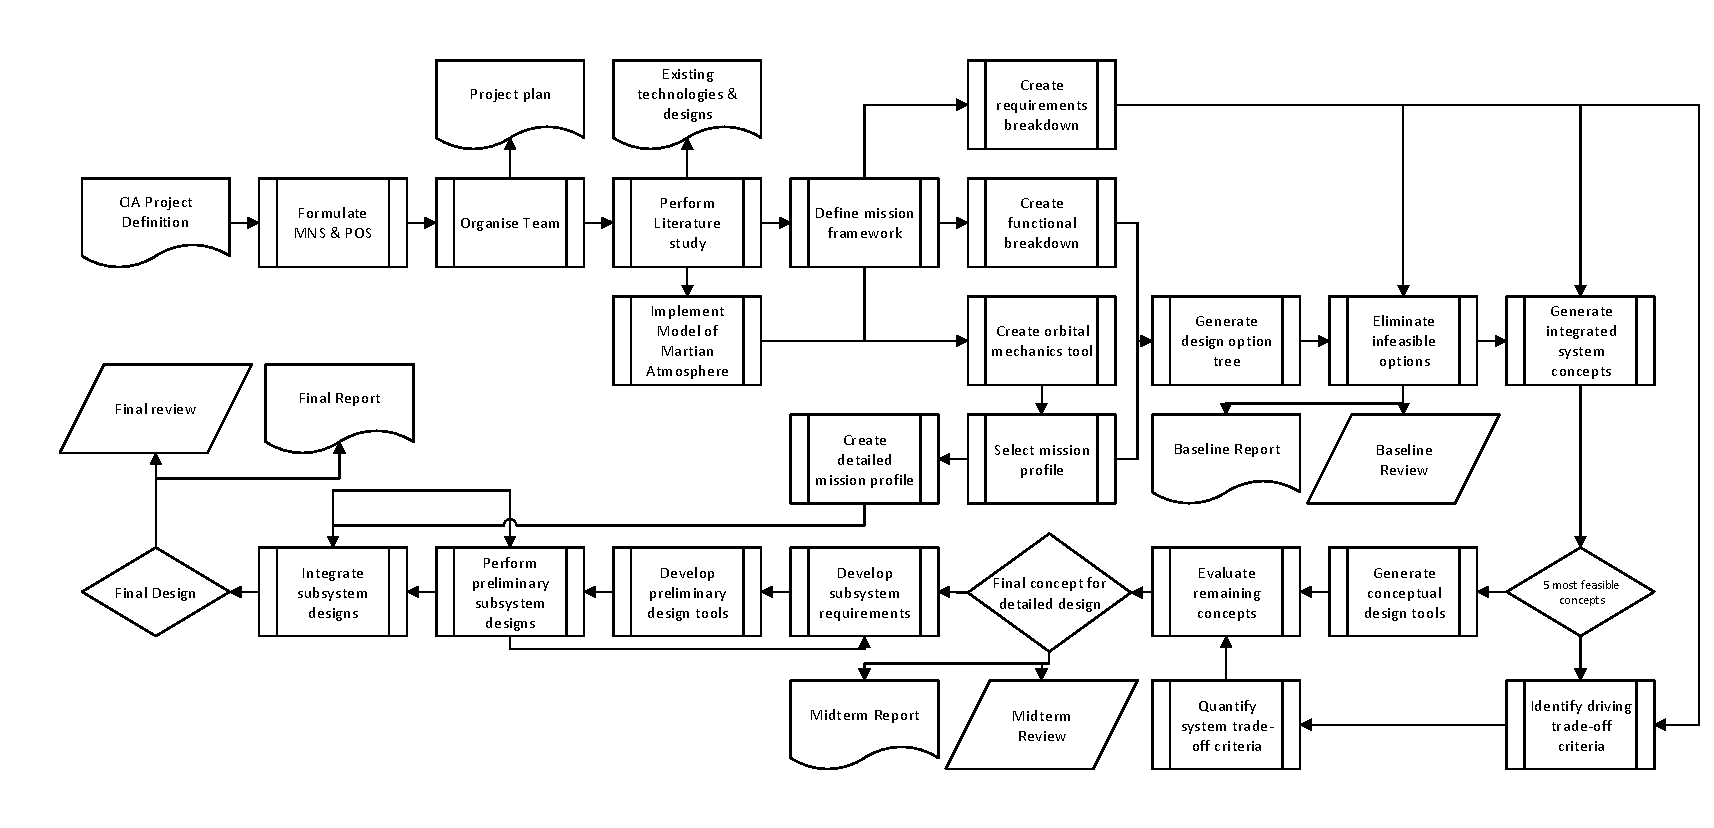
\includegraphics[scale=0.85]{Figure/WFD_MTR.pdf}
    \caption{\acrfull{wfd} of project}
    \label{fig:wfd}
\end{sidewaysfigure}
\section{Approach with respect to sustainable development}
\label{ch:sustain}

With a increasing awareness with respect to sustainable development it is important to consider the concepts sustainability. This section discusses the approach with respect to sustainable development of the \gls{hiad} design concepts at hand.
Masud et al. define development as being sustainable "by ensuring the needs of the present demands without compromising any power or ability of future generations to meet their own needs" \cite{Masud2011}.

Since the production series length of the controllable inflatable aeroshell is limited to very low numbers less emphasis is given to sustainable development when compared to (for example) a commercial passenger jet. As such the aeroshell's environmental impact is negligible and the sustainability of the concepts discussed in this report is not taken into account as a strong design driver. That is not to say sustainability is completely disregarded during product development. If for a certain design manufacturing methods are required that are very polluting these will be avoided and exchanged for less environmentally unfriendly, 'greener' methods. 
Not only sustainability on Earth is taken into account, but also the impact of a space mission to another orbital body on the environment of said body is considered. Special care will be given to prevent accidental contamination of other orbital bodies with organic lifeforms and other contaminants. This is in line with article IX of the Outer Space Treaty of 1967 \cite{UnitedNations2008}, enforced by the Committee on Space Research (COSPAR). In addition to preventing forward interplanetary contamination care will be taken to minimise the amount of space debris left behind in an orbit around Earth and Mars. 

The development of a controllable inflatable aeroshell can however contribute to making both planetary and interplanetary spaceflight more sustainable. Since implementing an inflatable aeroshell can contribute to reducing the total mass of a spacecraft this can reduce the required launcher mass and thereby the launch emissions. The differences with respect to sustainability between the different concepts to be analysed is very small and is thus not used as a separate element in the trade-off process.

Going back to the definition of sustainable development presented at the beginning of this chapter one can see that the measures taken during the design phase are indeed in line with sustainable development.
\section{Trade-off criteria}
\label{ch:tradeoff}
This chapter gives an overview of the trade-off process and the elements involved. It is essential that concepts are evaluated for their qualities important to the customer. While all concepts shall meet the requirements, freedom in the design space remains to allow for the best possible solution to maximize customer satisfaction. This freedom is expressed by the differing design options, customer satisfaction by a selected set of trade-off criteria. Each trade-off criterion is stated and thereafter briefly discussed in the sections below.

\subsection{Decelerator mass}\label{subsub:decelmass}
The (re-)entry vehicle consists of a decelerator, either in the form of a rigid heat shield and supporting structure or in the form of an inflatable heat shield and supporting structure and inflation system, and a payload module. Since total entry mass is constrained by launcher considerations, a reduction in decelerator mass will allow for a larger payload mass to be taken on-board. To fully exploit launcher mass-carrying capabilities, total entry mass is held at its maximum and increments in the two components making up total entry mass directly transfer from one to the other. It is highly desirable to maximize payload mass, since it is synonymous to maximizing the useful load-carrying capability of the (re-)entry vehicle. The latter allows either taking more payload in a fixed number of missions to Mars or taking a fixed total payload to Mars in a decreased amount of missions, thereby decreasing the total launches required. This translates to higher sustainability, by a decreased use of resources, and increased cost-effectiveness, by a decreased number of total launches and resulting total launch costs.

\subsection{Development risk}
Concepts with a lower development risk are preferable, since technology readiness directly affects schedule risk, cost risk and technical performance risk. Underdeveloped concepts inherently feature a larger amount of uncertainty. Eliminating this uncertainty requires additional resource expenditure, in the form of an increased number of test runs for example, thereby imposing a greater burden on available schedule time and monetary resources. In case the uncertainty would be left unexplored, technical performance would suffer by a decreased knowledge about product behavior and capability, increasing technical performance risk. To preserve mission reliability, concepts with a higher development risk require additional investigation and thereby carry additional resource and schedule loads. Moreover, in case these concepts are further explored and found to be ill-suited to the mission, a re-run of concept selection, analysis and design is required. It is therefore essential that development risk is as low as possible primarily for economical reasons.

\subsection{Deceleration time}
A decreased time to touchdown alleviates costs incurred by ground operations and mitigates physical taxation of human payload on-board. Ground operations are required to be fully active during entry operations and a decrease in entry duration will reduce the working hours and associated costs. Physical taxation is reduced by a shorter duration of high g-loads on human payload. A reduction in physical taxation will require less measures to counteract the negative effects thereof on the human body and widen the range of prospective capsule inhabitants by a reduction of physical requirements. As such, it is desirable that entry time is as small as possible, within the requirements imposed by the customer.

%Deceleration is maximized when the maximum tolerable acceleration is sustained throughout entry, as discussed in Chapter \ref{ch:astrocontrol}. Control is performed by a control system that alters the lift by changing the angle of attack of the vehicle, the performance of which increases for an increasing lift gradient. An increased performance of the control system leads to longer adherence to the 3-g limit imposed and thereby to a decreased deceleration time.

\subsection{Stability}
An increased vehicle stability is preferable, since a stable vehicle requires less control forces to counteract perturbations. A stable vehicle will react to a perturbation by an oppositely directed moment to revert itself to its equilibrium condition, where an increase in stability will bring about a larger reaction moment. This counters the perturbation faster than a less stable vehicle, while an unstable vehicle would increase the effects of the perturbation and bring it further from its equilibrium condition. It is desirable that the effect of perturbations is mitigated as much as possible, since these are unpredictable and bring about vehicle deviation from its intended trajectory. Stability is the preferable method of mitigation, since counteraction of perturbations by active control requires additional expenditure of power or propellant mass. 

%In the context of the two-dimensional orbit model, perturbances are considered in pitch direction and hence causing a change in angle of attack. A first indication for stability is decelerator static stability, measured in the moment coefficient derivative with respect to angle of attack. As discussed in Chapter \ref{ch:aero_analysis}, this parameter is obtainable using the developed aerodynamic analysis tool for each of the five concepts.
%An increased orbit controllability brings about greater freedom in trajectory selection and optimization on one hand and increases vehicle capability of counteracting perturbations on the other hand. While the latter capability is to be safeguarded in all designs in order to maintain minimum mission reliability, the former distinguishes concepts by a greater design efficiency. Increased controllability allows fine-tuning trajectories to a larger extent, such that trajectories can be optimized to induce smaller thermal and aerodynamic loads. Lowering peak loads allows design of a structure and \acrfull{tps} with lower design loads, thereby sized smaller than an equivalent structure and \gls{tps} sized for higher peak loads. This effects a decrease in decelerator mass, thereby increasing payload-carrying capability (see subsection \ref{subsub:decelmass}).




\section{Conceptual design options} \label{ch:options}
This chapter will discuss the five design concepts that will be considered in this report. First the selection of concepts based on the shape, mission duration and controls system design option trees is made. For the six configurations of the \gls{br} one is disregarded as it has no additional advantages over the other concepts. In section \ref{sec:conf} the five selected configurations are sketched and described. A simple load analysis is given in the form of \gls{fbd} to gain insight in the functioning of each of the concepts. The following five design are consequently used for analysis in the relevant chapters of this report. Finally the control systems corresponding to the each of the shape configurations are discussed in chapter \ref{sec:ccs}. A full definition of the control system is not yet given but is rather further detailed in the \gls{fr}.

\subsection{Concept selection}
 From the \acrfull{br} three \glspl{dot} were obtained for the design of the \gls{hiad}. In these designs concepts; shape, mission duration and control system are considered. This yielded a set of all the individual design options. These options are shown in Fig. \ref{fig:dotshape} to \ref{fig:dotduration}. From these \glspl{dot} a feasible set of design options can be obtained. In Fig. \ref{fig:dotshape} six deemed feasible concept configurations can be seen. This can consequently be combined with three possible control systems from Fig. \ref{fig:dotcontrol}. The mission duration varies for all concepts and is therefore considered separately for every design concept. The mission duration appears in the from of a trade of criteria discussed further in section \ref{ch:tradeoff} discussing the trade off criteria.

\begin{figure}[H]
%\centering
\hspace{-23mm}
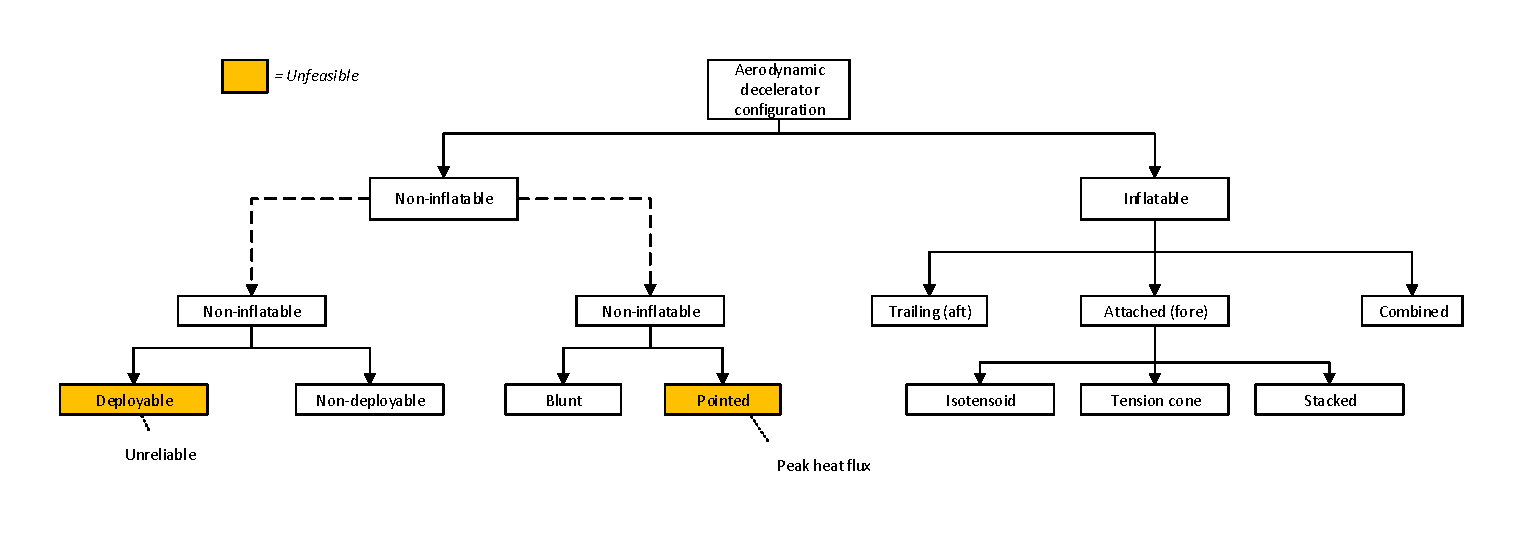
\includegraphics[width = 1.25\textwidth]{Figure/DOT_configuration.pdf}
\vspace{-5mm}
\caption{\acrlong{dot} for entry vehicle configurations}
\label{fig:dotshape}
\end{figure}

\begin{figure}[H]
\centering
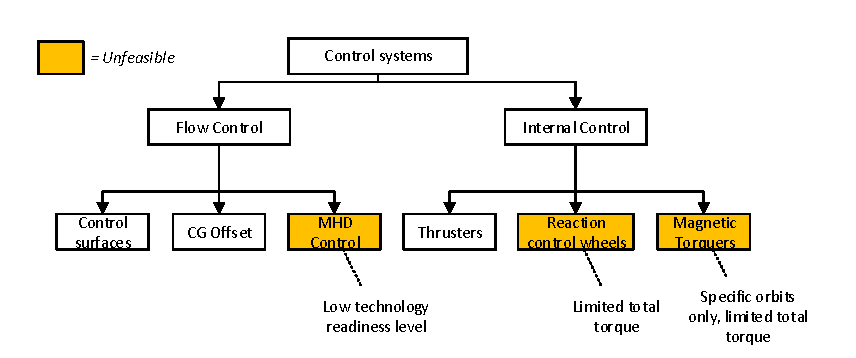
\includegraphics[width = 0.93\textwidth]{Figure/DOT_control.pdf}
\vspace{-5mm}
\caption{\acrlong{dot} for control systems}
\label{fig:dotcontrol}
\end{figure}

\begin{figure}[H]
\centering
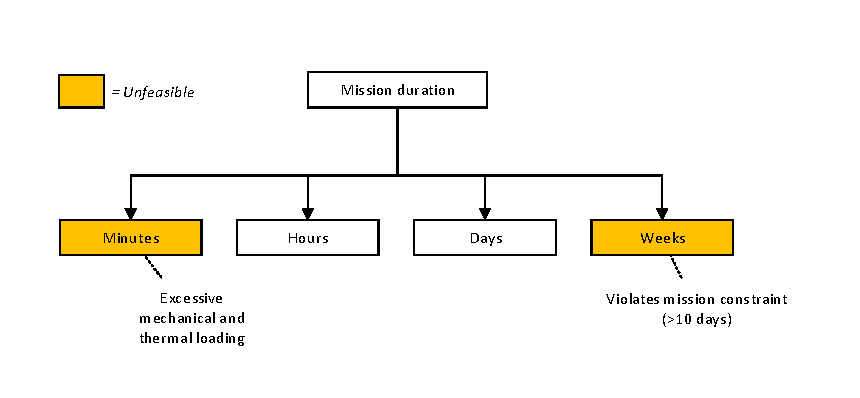
\includegraphics[width = 1.0\textwidth]{Figure/DOT_missionduration.pdf}
\vspace{-5mm}
\caption{\acrlong{dot} for mission duration}
\label{fig:dotduration}
\end{figure}

From the eighteen options yielded by combining the 6 feasible shapes and 3 feasible control systems shown in Figures \ref{fig:dotshape} and \ref{fig:dotcontrol} some may be disregarded immediately since they cannot practically be combined. For obvious reasons it is crucial that each concept configuration features at least one deemed feasible control system. From this point onward the concept shape will be considered leading. 

The control systems from Fig. \ref{fig:dotcontrol} are considered separately for each of these shapes. Due to infeasibility of exotic control concepts such as the, for now, deemed infeasible \gls{mhd} the control system can be integrated with each structure. This can be done since the control systems themselves do no longer require strict geometric properties as would be required by for example \gls{mhd} control.

Table \ref{tab:designconcepts} shows the design options that will be considered within this report. The check-marked control systems are further investigated for their feasibility and performance within section \ref{sec:ccs}. It must be noted that the control configurations of Table \ref{tab:designconcepts} feature the primary control mechanism. These may always be appended later on in the design process, after the trade-off, if additional control systems increase the overall systems performance. 

\begin{table}[H]
	\caption{Generation of design concepts}
	\label{tab:designconcepts}
	\centering
		\begin{tabular}{|p{0.3\textwidth}|p{0.14\textwidth}|p{0.14\textwidth}|p{0.14\textwidth}|} \hline 
			\textbf{Concept} & \textbf{Thrusters}	& \textbf{\gls{cg} offset} &  \textbf{Control surfaces} \\ \hline \hline
			Stacked toroid   & \cmark	& \cmark &  \cmark \\ \hline
			Isotensoid		 & \cmark	& \cmark &  \xmark\\  \hline
			Tension cone	 & \cmark	& \cmark &  \cmark \\ \hline
			Trailing ballute & \xmark	& \xmark &  \cmark \\ \hline
			Combined 		 & \xmark	& \xmark &  \cmark \\ \hline
			Rigid  		   	 & \cmark	& \cmark &  \cmark \\ \hline
		\end{tabular}
\end{table}

From Table \ref{tab:designconcepts} it can be noted that all shape configurations are deemed feasible for at least one control system. To yield a total of five concepts the combined concept is disregarded.
 It is considered to be too similar to a Trailing concept. A trailing concept will still require a heat shield in front of the payload and can therefore be considered, is some aspects, a combined configuration as well. It is therefore considered that a deployable inflatable at the front will have no additional advantage. A small deployable will have a similar performance as the trailing configuration, but features the additional complexity of the front inflation system. A large frontal inflatable will however place the aft inflatable in the wake making it effectively useless. Removing the aft declarator will however yield a "simple" stacked toroid, Isotensoid or tension cone configuration. For these reasons the trailing concept will not be considered. 
 
 The infeasible combinations of control systems are further detailed in \ref{sec:ccs}, together with a general description of each set of control system. 

\subsection{Concept configurations} \label{sec:conf}
In this section a the global configuration of each of the final five shapes is considered. They are sketched and described shortly in the sections below. Moreover a simple \gls{fbd} is provided to gain insight in, where applicable, the structural principle of each of the concepts.

\textbf{Stacked toroid}

Fig. \ref{fig:conc_stacked} and \ref{fig:fbd_stacked} show the stacked toroid concept. A stacked toroid configuration features multiple inflatables which are stacked together to form the aeroshell. These inflatables are consequently covered with a thermal protection layer. In this design the payload is placed aft of the aeroshell.\

\begin{figure}[H]
\centering
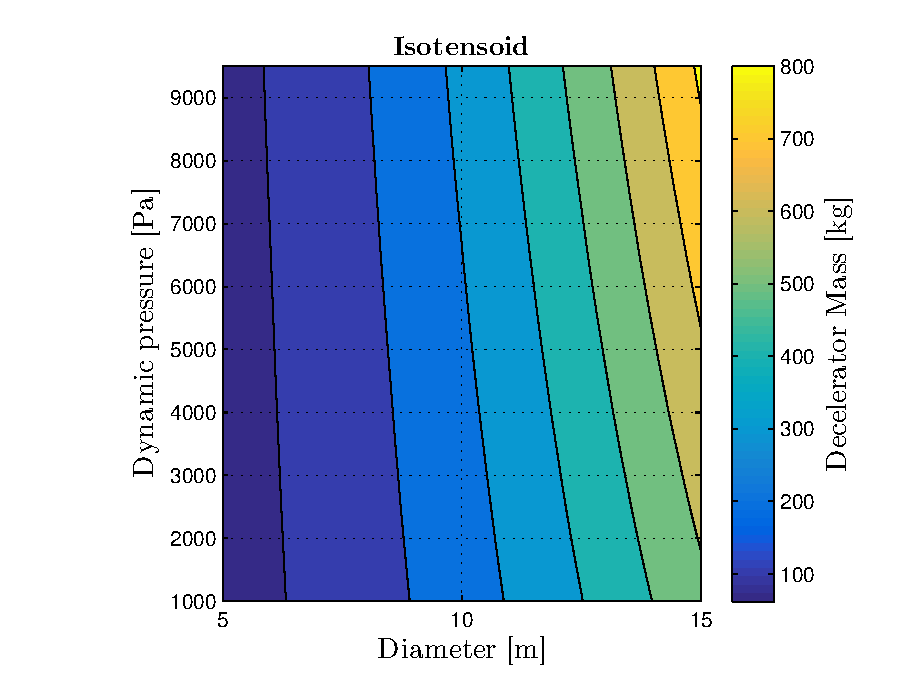
\includegraphics[width = 0.5\textwidth]{Figure/ISO_comp.eps}
\caption{A schematic view of a stacked toroid configuration}
\label{fig:conc_stacked}
\end{figure}

\begin{figure}[H]
\centering
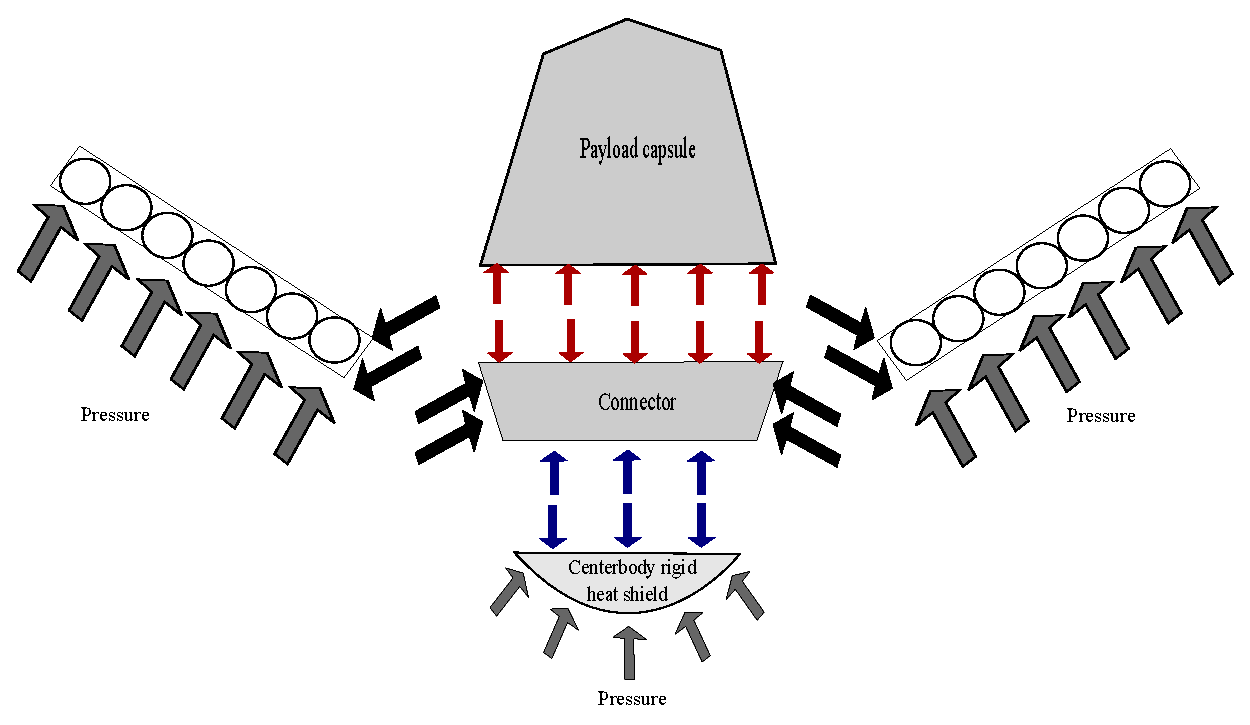
\includegraphics[width = 0.62\textwidth]{Figure/FBD_stacked.eps}
\caption{A \gls{fbd} of the stacked toroid configuration}
\label{fig:fbd_stacked}
\end{figure}


\textbf{Isotensoid}

An isotensoid configuration as displayed in Fig. \ref{fig:conc_iso} and \ref{fig:fbd_iso} features a single inflatable. This inflatable covers the whole of the payload. This inflatable is relatively large and is typically inflated using ram-air \cite{Smith2011}. 

\begin{figure}[H]
\centering
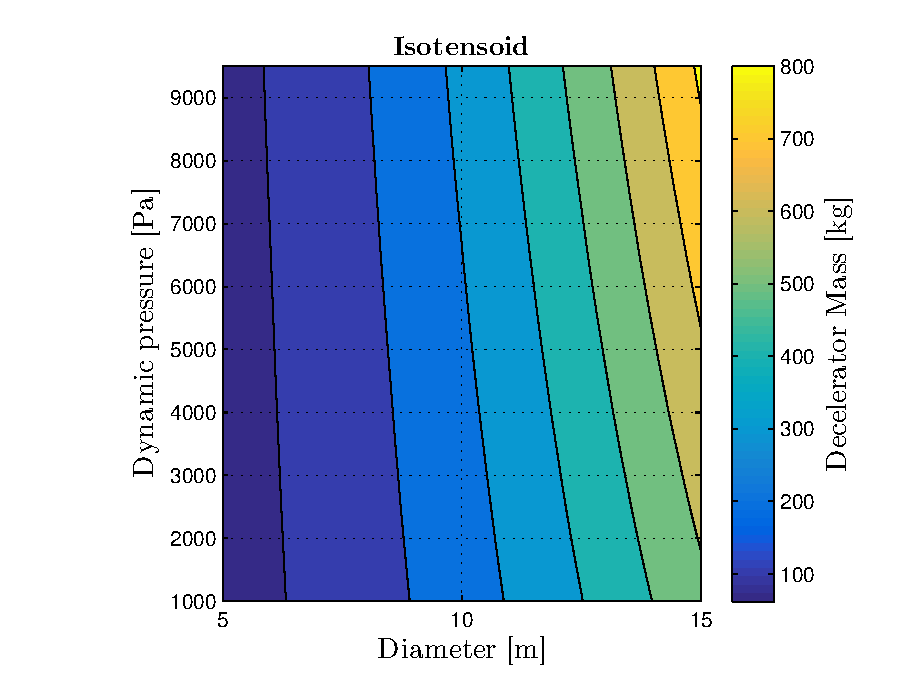
\includegraphics[width = 0.5\textwidth]{Figure/ISO_comp.eps}
\caption{A schematic view of a isotensoid configuration}
\label{fig:conc_iso}
\end{figure}

\begin{figure}[H]
\centering
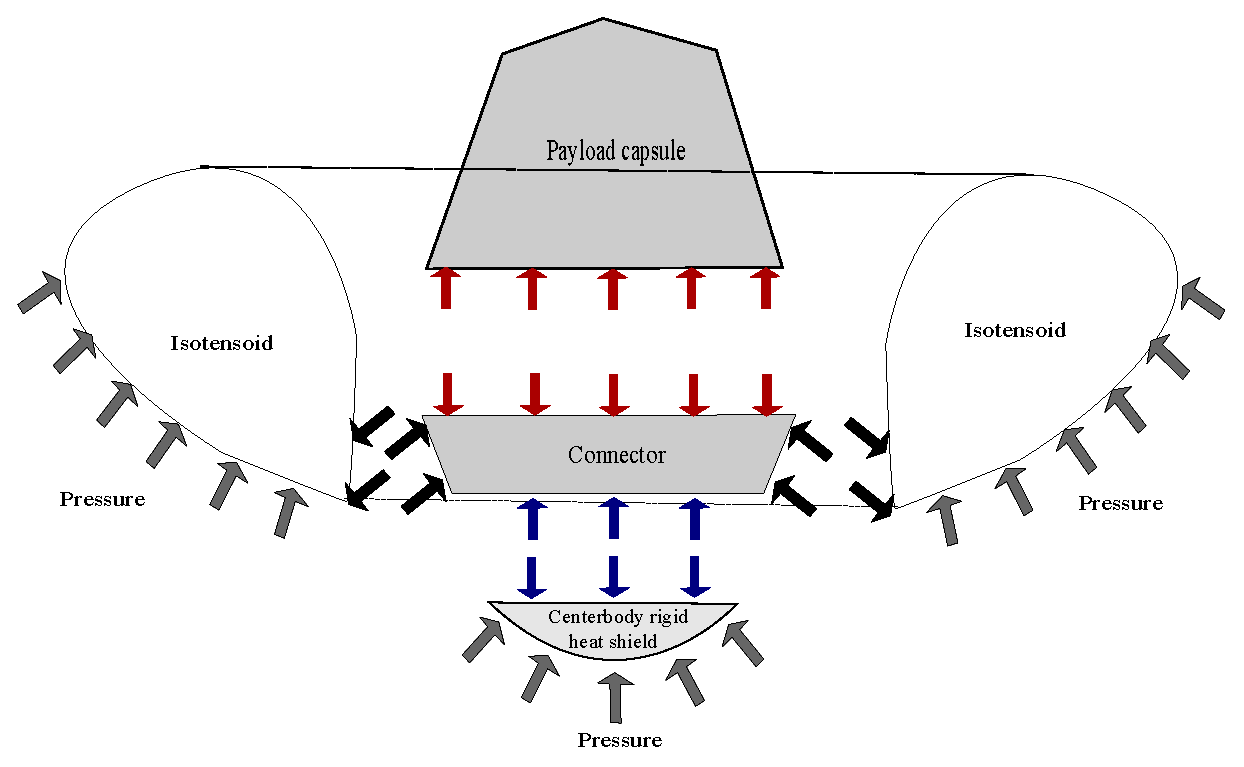
\includegraphics[width = 0.55\textwidth]{Figure/FBD_isotensoid.eps}
\caption{A \gls{fbd} of the isotensoid configuration}
\label{fig:fbd_iso}
\end{figure}

\textbf{Tension cone}

A tension cone, as shown in Fig. \ref{fig:conc_tension} and \ref{fig:fbd_tension}  again consists only of a single inflatable. In this case the inflatable is ring formed, using the ring to provide stiffness to a web spanned within. In this configuration the aeroshell is placed front of the payload, warping around it in some extend.

\begin{figure}[H]
\centering
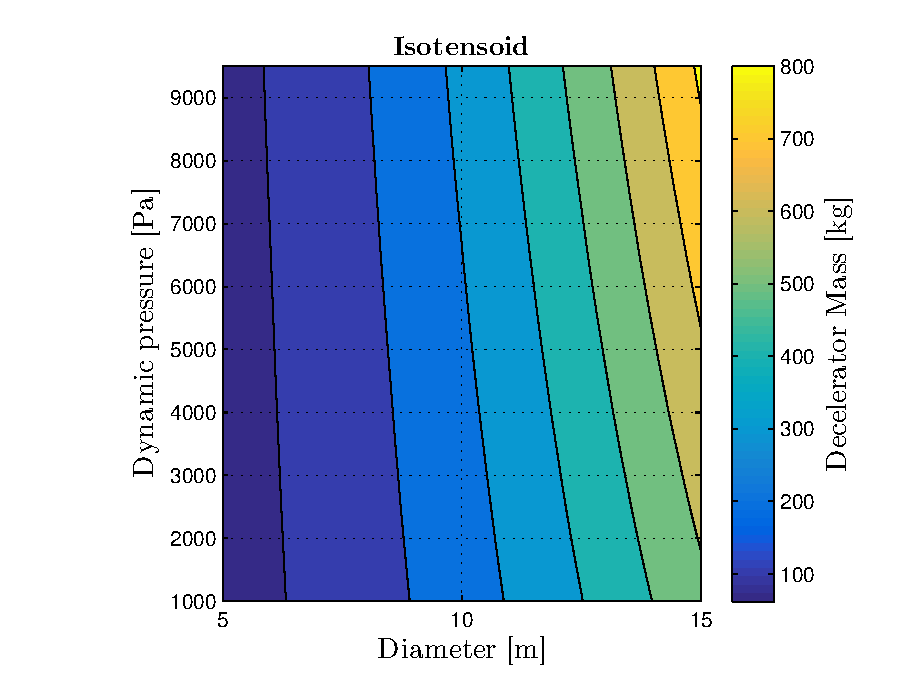
\includegraphics[width = 0.5\textwidth]{Figure/ISO_comp.eps}
\caption{A schematic view of a tension cone configuration}
\label{fig:conc_tension}
\end{figure}

\begin{figure}[H]
\centering
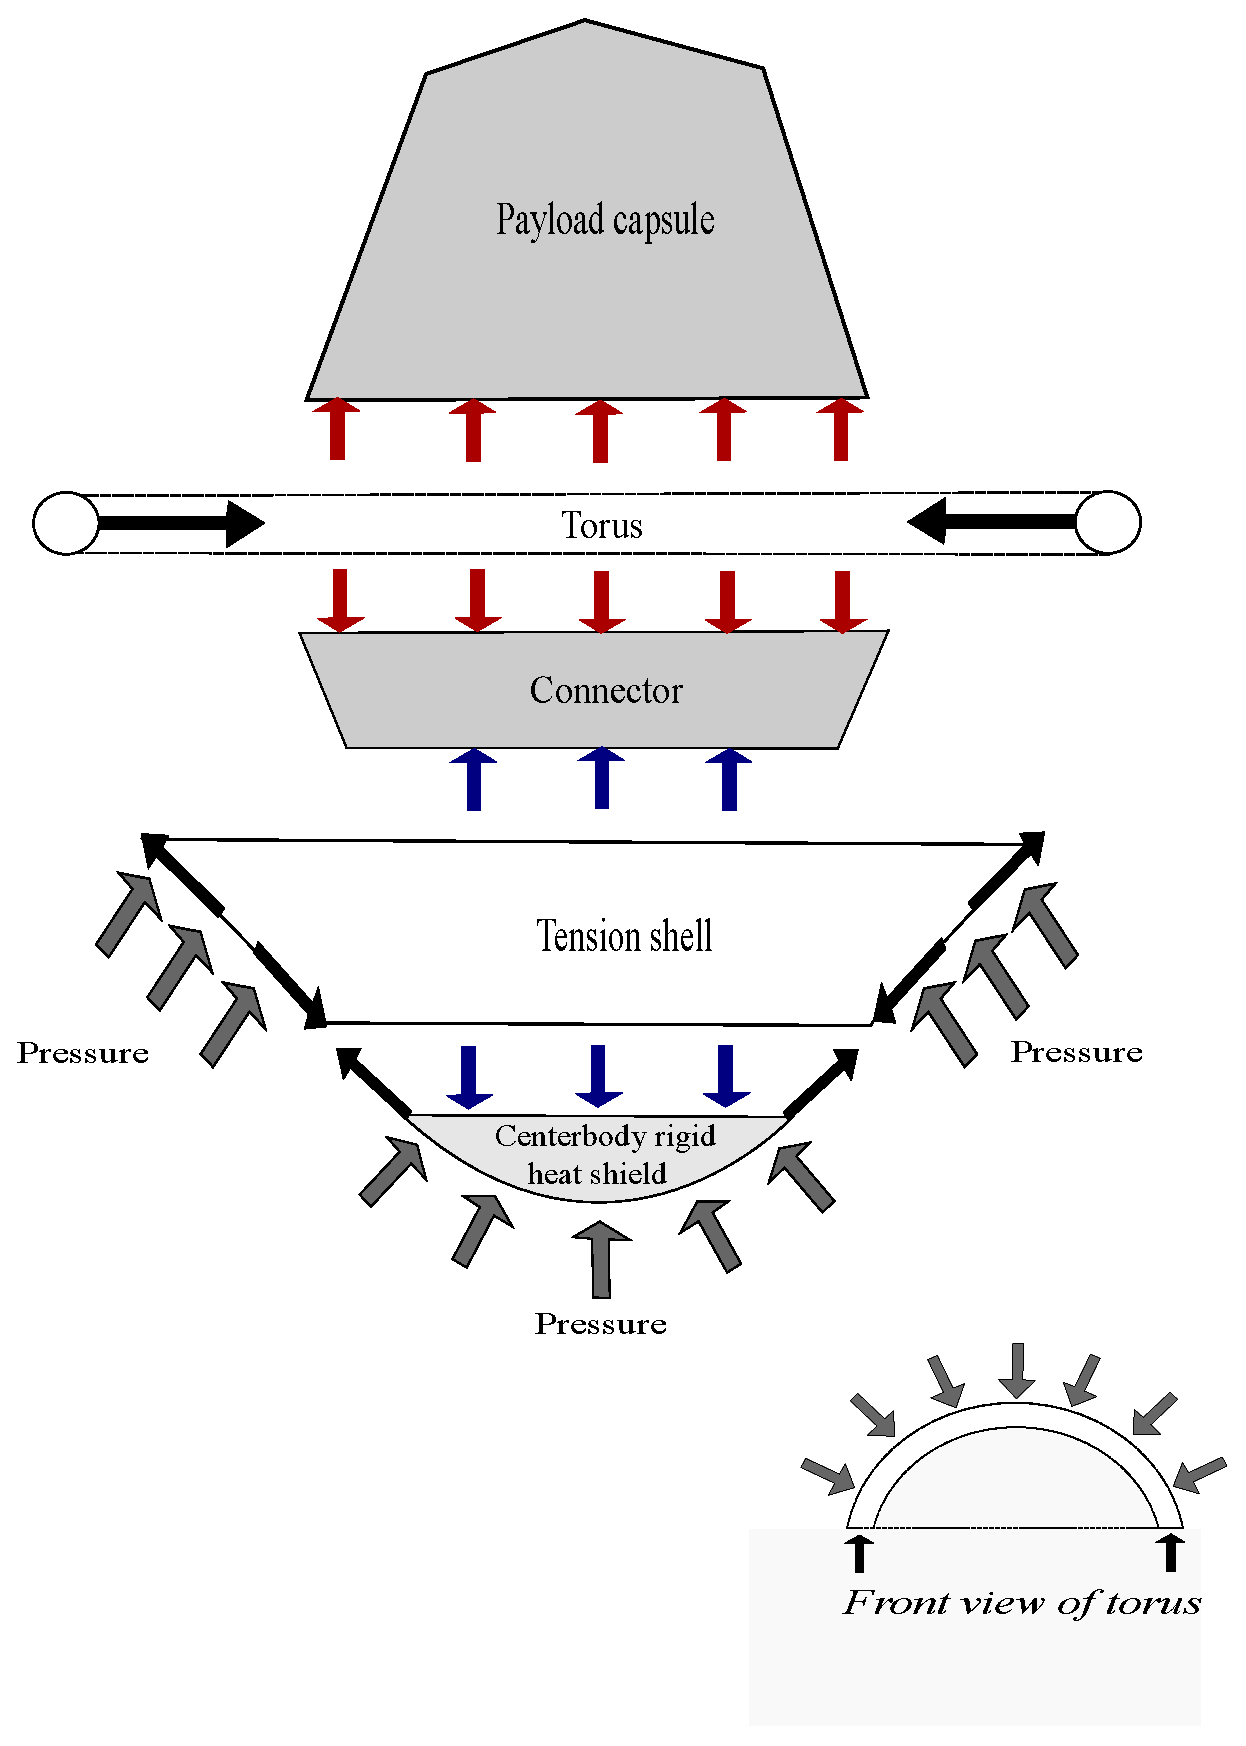
\includegraphics[width = 0.4\textwidth]{Figure/FBD_tensioncone.eps}
\caption{A \gls{fbd} of the tension cone configuration}
\label{fig:fbd_tension}
\end{figure}

\textbf{Trailing}

Fig. \ref{fig:conc_trailing} \ref{fig:fbd_trailing} show a trailing configuration. A Trailing configuration consist of two parts. A aft placed inflatable, typically referred to as the the trailing, and a front placed rigid heatshield. Since the inflatable is aft placed the payload is directly exposed to the atmosphere requiring the addition of the rigid heatshield. The shock waves induced by the front of the payload consequently create a wake aft of the payload. A typical trailing device is therefore ring formed to stay out of this wake is also displayed by Fig. \ref{fig:conc_trailing}. This is also the trailing configuration as treated within this report.

\begin{figure}[H]
\centering
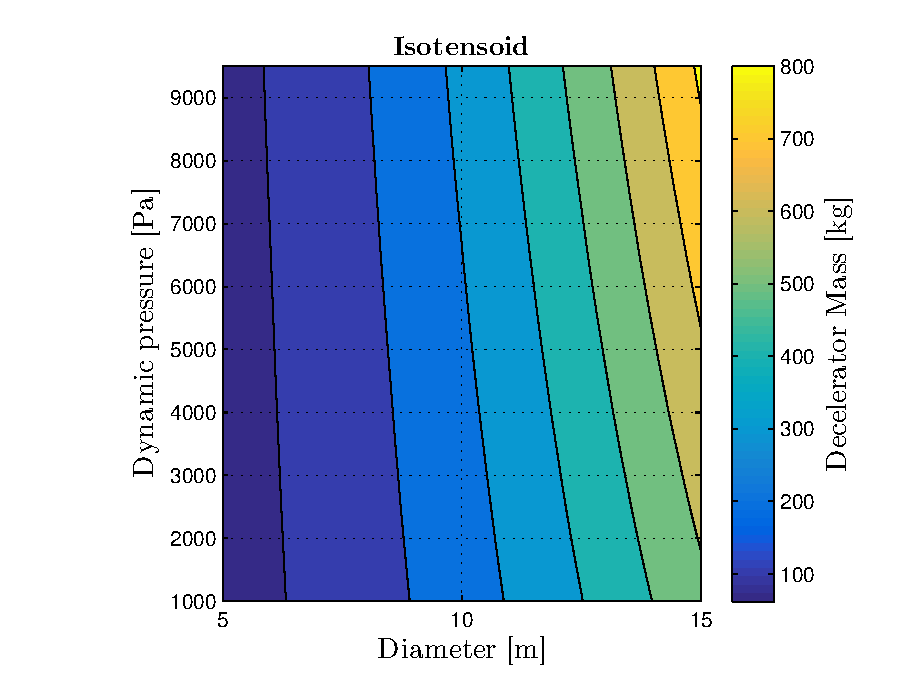
\includegraphics[width = 0.5\textwidth]{Figure/ISO_comp.eps}
\caption{A schematic view of a trailing configuration}
\label{fig:conc_trailing}
\end{figure}

\begin{figure}[H]
\centering
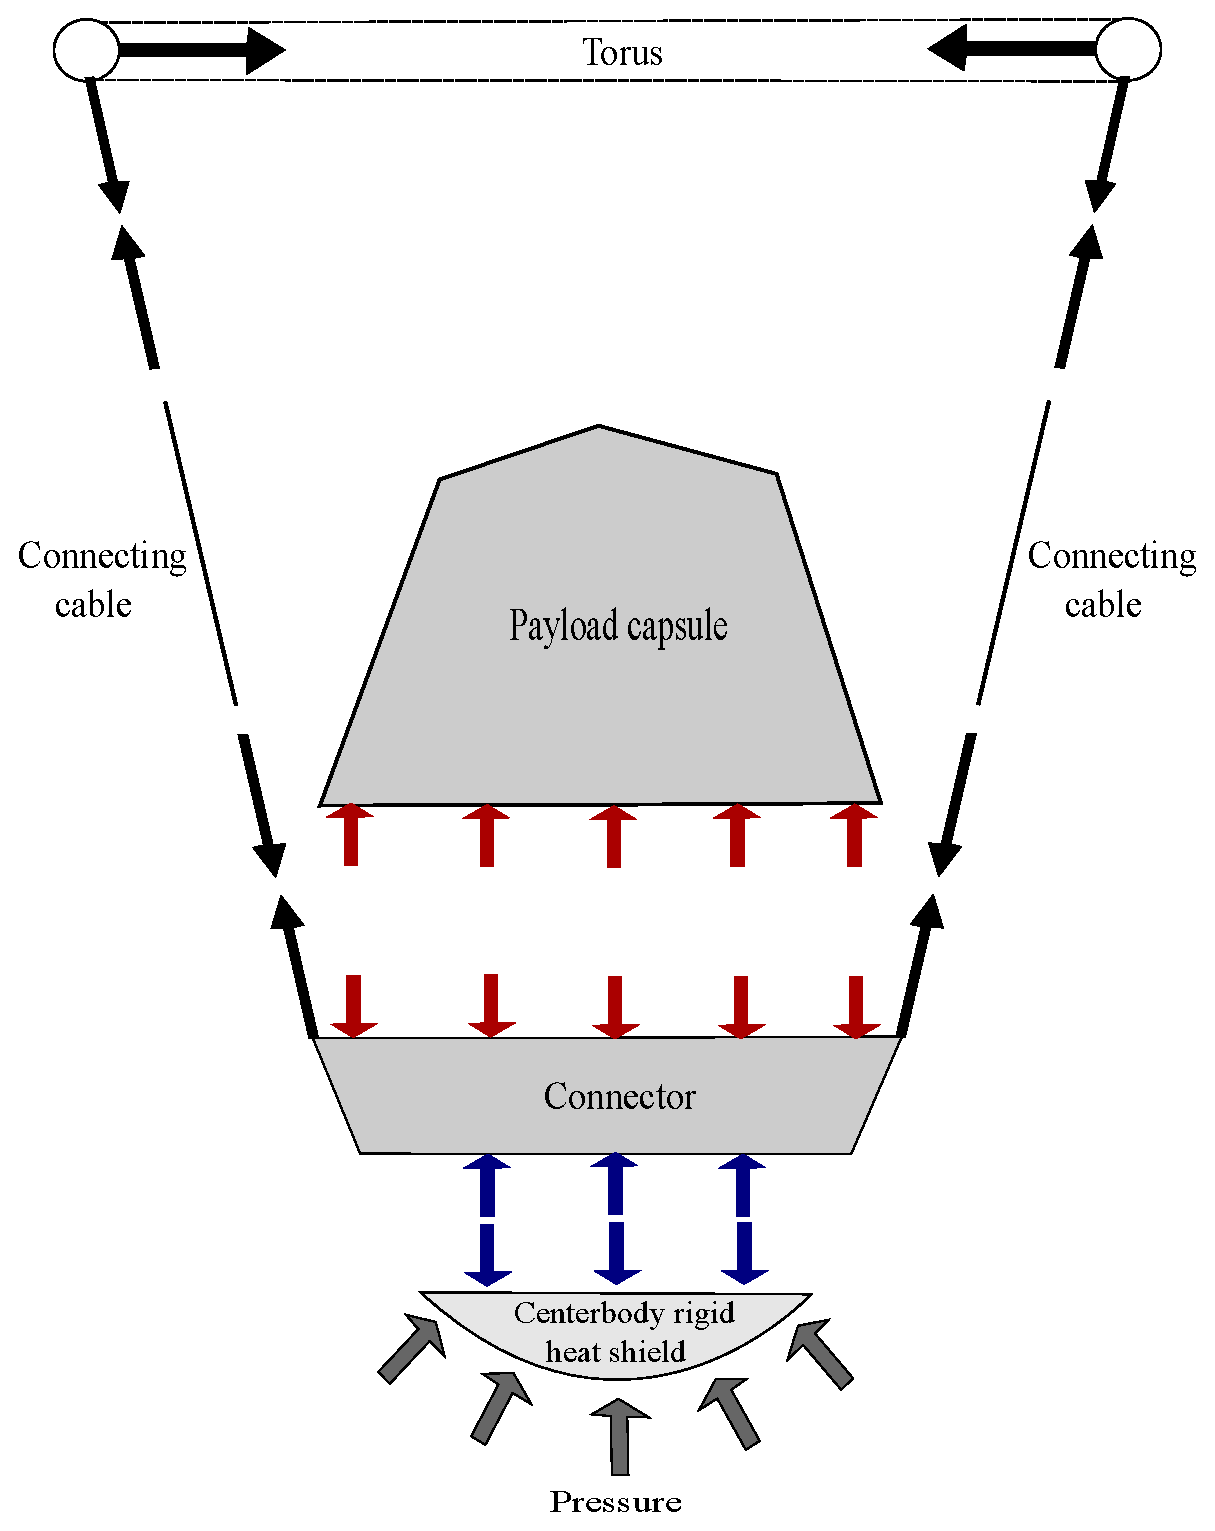
\includegraphics[width = 0.4\textwidth]{Figure/FBD_trailing.eps}
\caption{A \gls{fbd} of the trailing configuration}
\label{fig:fbd_trailing}
\end{figure}

\textbf{Rigid}

The rigid configuration is the most typical configuration and frequently used by returns to the earth atmosphere such as in the Apollo, Soyuz or planned Orion mission. Fig. \ref{fig:conc_rigid} and \ref{fig:fbd_rigid} show the Rigid configuration. This design features a rigid heatshield in front of the payload and is the only concept featuring no inflatable parts.

\begin{figure}[H]
\centering
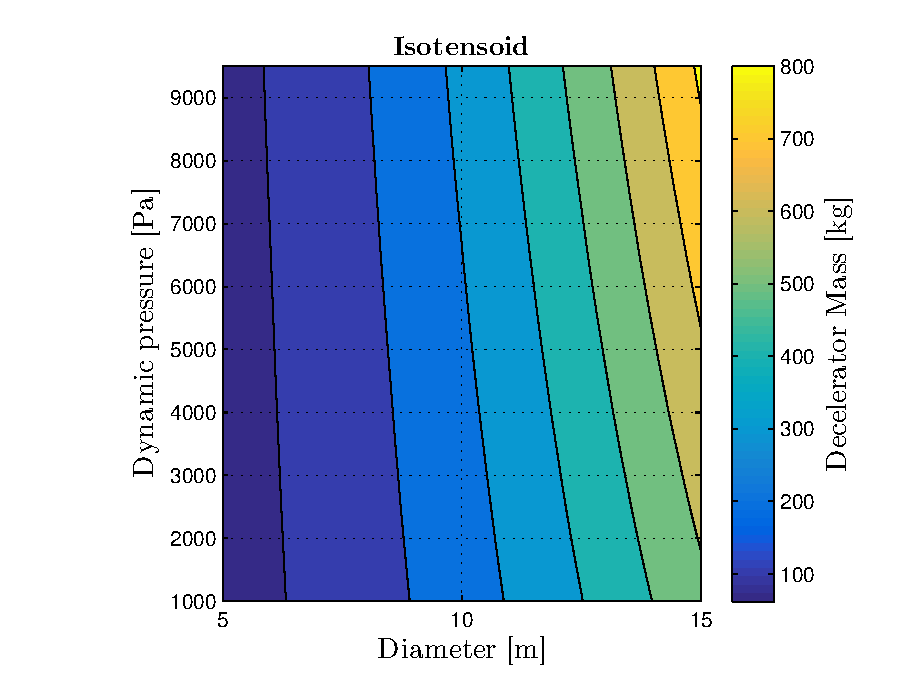
\includegraphics[width = 0.5\textwidth]{Figure/ISO_comp.eps}
\caption{A schematic view of a rigid configuration}
\label{fig:conc_rigid}
\end{figure}

\begin{figure}[H]
\centering
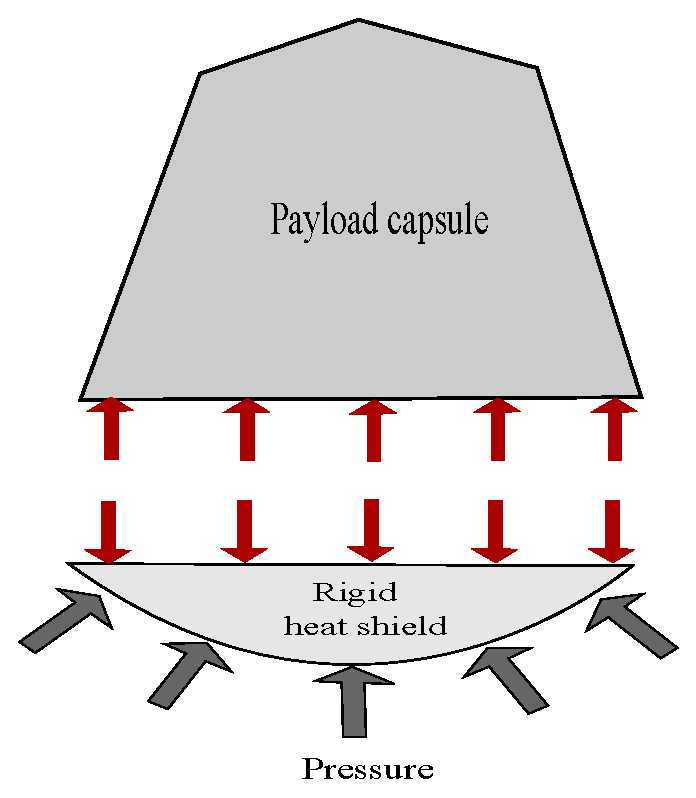
\includegraphics[width = 0.3\textwidth]{Figure/FBD_rigid.eps}
\caption{A \gls{fbd} of the rigid configuration}
\label{fig:fbd_rigid}
\end{figure}

\subsection{Concept control systems} \label{sec:ccs}
This section discusses the control systems for each of the control systems of the design option tree. This is related to the shapes of each of the concepts also serving to explain the checkmarks and crosses of Table \ref{tab:designconcepts}. 

The control surfaces are not yet further detailed within the midterm report. Development risk and control system mass is however taken into account by considering the feasible control concepts and by considering the aerodynamic properties of the concepts. The latter is detailed in Chapter \ref{ch:aero_analysis}.

\subsubsection{\gls{cg} offset}
A centre of gravity offset can be used in two ways. A static centre of gravity offset which is typically employed, and a actively employed \gls{cg} offset system. The latter is already demonstrated in the \gls{irve}-3 mission \cite{Dillman2012}, however considering smaller payload module mass fractions. Applying a \gls{cg} offset yields  a non symmetric body, creating a lift vector. In a \gls{cg}-offset control system this property is actively used for the control of the system. 

The use of a \gls{cg} does however have speed limitations as changes is centre of gravity are slow.

The usage of a active \gls{cg} offset systems for the trailing and combined configuration is not deemed feasible due to the existence of aft the elements which are connected with a non rigid combination.

\subsubsection{Thrusters}
Thrusters are the only deemed feasible internal control system and is hence always featured on the spacecraft. For the part of the mission up to the first entry into the Martian atmosphere thruster will thus be used in any case. Thrusters can however also be employed as a primary control surface for which the mass and usage of the systems is obviously increased.  

Thruster are deployed in pairs for the control of the spacecraft such that they can deliver pure torque. The amount of torque is a linear function of the relative distance between the thrusters and is constrained for this design by launcher constraints. 

In terms of development risk thrusters are frequently used and feature minimal risk.

Thrusters are not considered for the trailing and combined configuration. Due to the aft elements of these designs thruster cannot be considered as the primary control mechanism. Due to the large moments of inertia (due to aft elements) and very high stability of the aft systems (e.g. compare to a parachute) thrusters cannot be considered due their inefficiency. 

\subsubsection{Control surfaces}
Control surfaces have been subdivided into two forms; body flaps and morphing of the whole structure, which are both covered below.

\paragraph{Body flaps}
A control system with body flaps features deployable surfaces to control the flow around the spacecraft. Body flaps have previously been deployed at for example the Space Shuttle missions. It must however be noted that the usage was limited to lower Mach numbers at higher atmospheric densities. As such it is possible control concept for the rigid structure.

Body flaps on inflatable structures have not yet been featured and are not deemed feasible. Since body flaps need to based inside the flow positioning is not possible. In these designs the inflatable is the part placed within the flow. Do to the nature of deployment and the structural layout of these systems body flaps are not deemed feasible.

The usage of body flaps for the Mach numbers considered would also incur a significant development risk.

\paragraph{Morphing}
In morphing concepts the whole external shape is changed to control the spacecraft. This is not possible for rigid structures as no morphable parts exist, from the perspective of rigid decelerator structure. 
 For the inflatable structures morphing is deemed possible for with the exception of the isotensoid design and is already being investigated \cite{Hughes2011}. In the isotensoid design the whole outside is covered by inflatable. The whole inflatable can thus only e formed by usage of the gas inside. This is however not deemed possible due to the usage of ram-air as inflation mechanism.

Morphing of the trailing ballute configuration would be done via the payload-ballute connection much like for example a parachute.

In terms of development risk morphing of the structure is mostly at a very early conceptual phase posing significant development risks.
\section{Design interfaces} \label{ch:di}

This chapter discusses the design interfaces. First off, in section \ref{sec:N2} the interfaces between the different subsystems or departments which are considered during the design are given and discussed. This is appended by the design interfaces which needs to be considered during the operation of the mission in the form of a communication flow diagram in section \ref{sec:comflow}.

\subsection{Subsystem design interfaces} \label{sec:N2}
This section defines the interfaces between the different subsystems of the \gls{hiad}. The interfaces are defined in a similar manner as the technical work division of chapter \ref{sec:org}. This subdivision is trajectory \& control, aerodynamics, thermodynamics and structure.  The interfaces are illustrated in the form of a N2 chart as displayed in Fig. \ref{fig:N2} and will subsequently be discussed from the perspective of required inputs per subsystems.

\begin{figure}[H]
\centering
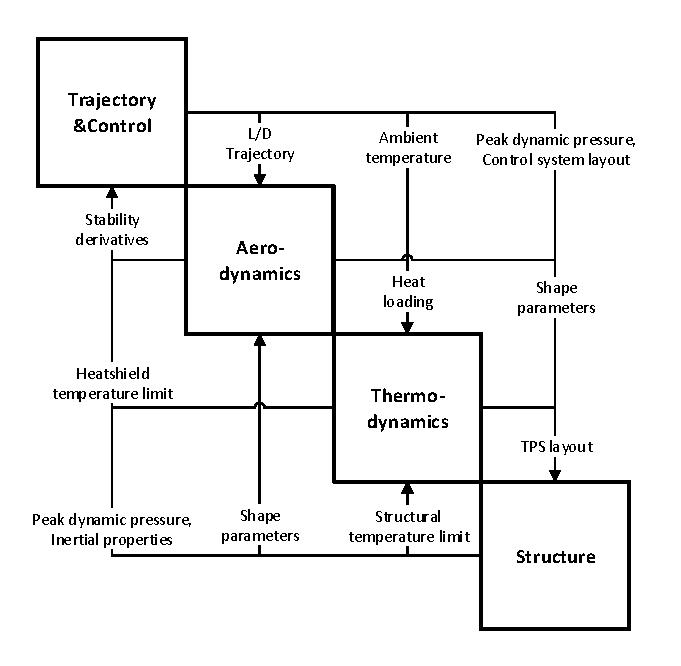
\includegraphics[width = 0.8\textwidth]{Figure/N2.pdf}
\caption{N2 of the interfaces in the \gls{hiad} design}
\label{fig:N2}
\end{figure}

\subsubsection{Trajectory \& Control}

The trajectory and control department or subsystem is one of the main drivers for the requirements of the individual subsystems. Outputs are mainly derived from the trajectory and control analysis although the inputs are also of crucial importance. 

The trajectory and control department requires stability derivatives in order to analyse the trajectory possibilities. Stability derivatives are considered in the broadest sense, also including other aerodynamic values such as \gls{sym:CD}\gls{sym:A}, \gls{sym:CL}\gls{sym:A} and \gls{sym:CM}\gls{sym:A} although these values are not actual derivatives. The input from the control department is  best summarized as below.

\begin{itemize}
\item Best if control dep. fills this in.
\item ??
\end{itemize}

As the control department and aerodynamic department become integrated the trajectory will be actively controlled in order to stay within the performance limits. For this purpose an additional heat shield temperature limit is required. The temperature limit will function as a constraint on the maximum possible deceleration.

Finally the inertial properties, such as for example the mass moments of inertia, and peak loads are provided by the structural department. The peak loads are supplied in the form of a peak dynamic pressure and functions as an additional constraint on the possible orbits. The inertial properties are used for simulation in the orbital analysis. 

\subsubsection{Aerodynamics}
The aerodynamics department provides two main functions. Providing stability derivatives which are required for the orbital calculations, and providing the thermal loads. 
For the former, stability derivatives are again considered in the broadest sense as discussed above. 

The trajectory input is also considered in very broad sense. The full trajectory yields a Machnumber, velocity and atmospheric properties all as a function of time which are required as a input for the Aerodynamic calculations. Note that the atmospheric properties follow from the location in the trajectory via the \gls{nasa} \gls{marsgram} software\cite{Justus2001}.

The actual shape of the system may differ slightly from the specifications as defined by the aerodynamic department itself. As such the aerodynamic department requires additional input from the structural department for the exact shape specification. This can be seen in the N2 chart as rather direct iteration loop between these two subsystems.

\subsubsection{Thermodynamics}
The main inputs for the thermodynamics department is the heat loading as function of time combined with a ambient atmospheric temperature. Moreover a temperature limit is required for the point to which the structure needs to be cooled down. This is value provided by the structure department which joins the \gls{tps} and the payload module.

\subsubsection{Structure}

The structure is sized on the structural loads. These structural loads follow mainly from the peak dynamic pressure and control forces from the trajectory and control department. Moreover from the thermodynamics department a heatshield \gls{tps} layout is defined which need to be fitted onto the structure and needs to be taken into account. 

The control forces are very dependent on the type of control system implemented. As such the type of control system implemented has its inputs on the structural subsystem as well as the applied control forces. 

Finally a shape is defined by the aerodynamics department for which the structure needs to be sized. 

\subsection{System communication flow} \label{sec:comflow}
Communication flow primarily takes place with respect to trajectory sensing and control. In order to adhere to a certain trajectory and to counteract perturbations, alterations in vehicle dynamics are required. These alterations are performed by actuators, as investigated in Chapter \ref{ch:astrocontrol}. The magnitude and direction of the alterations are determined by an on-board computing unit, by a comparison with the actual attitude as provided by attitude sensors mounted on the (re-)entry vehicle. Trajectory and attitude information is communicated to ground control via a Telemetry and Command Unit. A fail-safe system is included to take over computer functions in case of computer failure. This communication flow is depicted in Fig. \ref{fig:comflow}.

\begin{figure}[H]
\centering
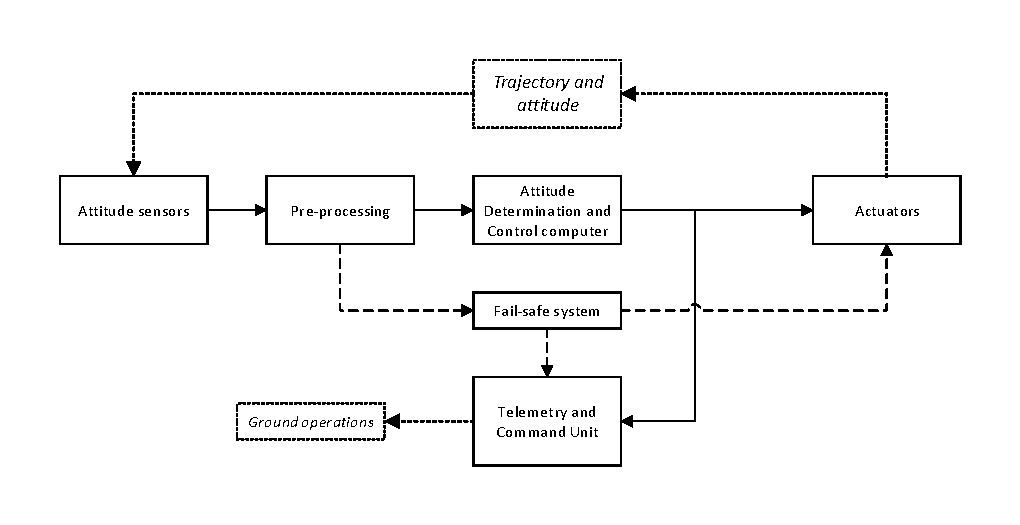
\includegraphics[width = 0.8\textwidth]{Figure/CommunicationChart.pdf}
\caption{Communication flow of control subsystem}
\label{fig:comflow}
\end{figure}


\section{Astrodynamics \& control tool development}
\label{ch:astrocontrol}
In this chapter the development of a tool for astrodynamics and control is described. The tool calculates the trajectory of the spacecraft for varying initial conditions and aerodynamic properties. With the information extracted from this tool requirements**maybe requirements is not the right word** for the control systems can be determined. Based on these requirements the different control systems available for the different concepts (which are presented in chapter \ref{ch:options}) can be weighed off in a trade-off in chapter \ref{ch:tradeoff}.

In this chapter first the purpose of the tool will be explained in section \ref{sec:astropurpose}. In sections \ref{sec:astrogov} and \ref{sec:astrowp} working principles of the tool are explained and the equations the tool is based on are presented. To ensure the tool calculates what it is supposed to calculate and to ensure this happens accurately enough in section \ref{sec:astrovv} the verification and validation of the tool is done. In section \ref{sec:astroref} performance of current day control systems are investigated. This performance is compared to the calculated needed performance to come to a conclusion in section \ref{sec:astrores}. Section \ref{sec:astrores} also presents some other results of the tool which are used as input for tools calculating i.e. structural mass.

\subsection{Purpose of tool development}
\label{sec:astropurpose}
***intro***\\
***No other tool publicly available***\\
***Determine the required Aerodynamic characteristics to create an acceptable window of entry***\\
***Investigate the need for \& effect of control***\\

\subsection{Governing equations}
\label{sec:astrogov}
***intro***\\
***Kepler for hyperbolic: Vis-Viva, polar expression of hyperbola, tangent to hyperbola)***\\
***Forces give accelerations: like in baseline + Jerk***\\
***Kepler for elliptic: symmetry***\\

\subsection{Working principles of the tool}
\label{sec:astrowp}
***intro***\\
***Flowchart + very short explanation***\\

\subsection{Verification \& validation}
\label{sec:astrovv}
***intro***\\
***sensitivity analysis: very sensitive to initial location, thus for now assumed initial location closer***\\
***discretisation error: error for different dt***\\
***Compare numerical results with Kepler, should be the same for rho=0***\\
***Validation through checking if output values are approximately the same as reference cases (peak dynamic pressure)***\\

\subsection{Performance of control systems}
 \label{sec:astroref}
***intro***\\
***Moment or dalpha/dt that control systems (cg offset, thrusters, control surfaces) can create***\\
***Weight estimate of each control system (per concept if needed)***\\

\subsection{Results \& Conclusions}
\label{sec:astrores}
***intro***\\
***Plot of a trajectory***\\
***Plots of output variables for that particular trajectory***\\
***Results of needed CLmax, dalpha/dt, dCL/dalpha***\\
***Conclusion on which control system (implemented in which concept) can perform as such***\\
***Conclusion on weight the control systems will bring along***\\
***State values for in trade-off matrix***\\
\section{Aerodynamic concept analysis}
\label{ch:aero_analysis}
In order to analyse the aerodynamic characteristics of the proposed concepts a software tool was developed. This chapter will deal with the development and implementation of this program. The aerodynamic tool is developed to be able to assess the performance of the different system concepts on the different trade-off criteria as defined in Chapter \ref{ch:tfsum}: the lift gradient \gls{sym:cla-alpha} relates to the deceleration time and the moment stability \gls{sym:cma-alpha} relates to the static stability of the decelerator. In order to calculate these values, the concept shapes are discretised in triangles, and for each triangle the pressure coefficient \gls{sym:cp} is calculated. This can then be integrated over the surface to obtain lift, drag and moment. Also, the maximum heat flux \gls{sym:qw} is determined for each concept, which is used to determine the thermal protection system mass. 
The chapter will start with a description of the analysis method used to determine the different aerodynamic properties of the various concepts in section \ref{subsec:aerotool}. The verification and validation of the analysis tool is discussed in section \ref{subsec:aeroverval}. Finally the developed analysis method is used to analyse the various system concepts and generate the required data for the trade off. 

\subsection{Development of aerodynamic analysis tool}
\label{subsec:aerotool}
For analysing the aerodynamic characteristics of each concept the modified Newtonian method will be used. This method relates the inclination angle $\gls{sym:chi}$ of a flat plate with respect to an incoming flow to the magnitude of its coefficient of pressure, as shown in Equation \ref{eq:modnewtonian} \cite{AndersonJr.2006}.
\begin{multicols}{2}
\begin{equation}
\gls{sym:CP}=\gls{sym:CP}_{max}sin^{2}(\gls{sym:chi})
\label{eq:modnewtonian}
\end{equation} \break
\begin{equation}
\gls{sym:CP}_{max}=\frac{p_{O_{2}}-p_{\infty}}{\frac{1}{2}\rho_{\infty}V_{\infty}^{2}}
\label{eq:cpmax}
\end{equation}
\end{multicols}
In equation \ref{eq:modnewtonian} $\gls{sym:CP}_{max}$ is the value of $\gls{sym:CP}$ in the stagnation point of an arbitrary body. Since the stagnation point is per definition located behind a normal shock its value can be found from the normal shock relations. The result of doing this is shown in Equation \ref{eq:cpmax}. Here $p_{O_{2}}$ denotes the total pressure in the stagnation point and can be found using Equation \ref{eq:po2} \cite{AndersonJr.2007}.

\begin{equation}
\frac{p_{O_{2}}}{p_{\infty}}=\left(\frac{(\gls{sym:gamma}+1)^{2}M_{\infty}^{2}}{4\gls{sym:gamma} M_{\infty}^{2}-2(\gls{sym:gamma}-1)}\right)^{\frac{\gls{sym:gamma}}{\gls{sym:gamma}-1}}\left(\frac{1-\gls{sym:gamma}+2\gls{sym:gamma} M_{\infty}^{2}}{\gls{sym:gamma}+1}\right)
\label{eq:po2}
\end{equation}

Furthermore it can be noted that $\frac{1}{2}\rho_{\infty}V_{\infty}^{2}=\frac{\gls{sym:gamma}}{2}p_{\infty}M_{\infty}^{2}$ \cite{AndersonJr.2007}. Combining this with Equation \ref{eq:cpmax} produces Equation \ref{eq:cpmaxfinal}, where the ratio $\frac{p_{O_{2}}}{p_{\infty}}$ can be calculated using Equation \ref{eq:po2}.

\begin{equation}
C_{p_{max}}=\frac{2}{\gls{sym:gamma} M_{\infty}^{2}}\left(\frac{p_{O_{2}}}{p_{\infty}}-1\right)
\label{eq:cpmaxfinal}
\end{equation}

By dividing the surface of the body to be analysed into many triangular elements the pressure coefficient distribution of said body can be determined numerically. A velocity magnitude is given as input, together with the angle of attack \gls{sym:alpha} and sideslip angle \gls{sym:beta}. Following this the outward surface normal vector is computed in Cartesian coordinates for every element, after which the velocity unit vector is computed with Equation \ref{eq:unitV}. To determine $sin(\gls{sym:chi})$ for every element the dot product of the velocity unit vector with the surface normal vector is then taken, as shown in Equation \ref{eq:dotproduct}.
\begin{multicols}{2}
\begin{equation}
\gls{sym:Vhat}=\frac{\gls{sym:Vv}}{\gls{sym:V}}
\label{eq:unitV}
\end{equation} \break
\begin{equation}
sin(\gls{sym:chi})=\gls{sym:Vhat} \bullet \gls{sym:n}
\label{eq:dotproduct}
\end{equation}
\end{multicols}
Using $C_{p_{max}}$ and $sin(\gls{sym:chi})$ the \gls{sym:CP} for every surface element is calculated, after which it is multiplied with the element area and the element surface normal vector. This results in an elemental pressure force in three dimensions from which the lift and drag forces can be determined. By then summing the resultant forces for all elements the total body forces are found. Next to the body forces the resultant aerodynamic moment can also be found. For this the location of the \acrfull{cg} is used as input, after which the moments about the \gls{cg} caused by the force on each element can be summed. 

Two notes are made here with regard to the results produced by the Newtonian flow method:
\begin{itemize}
	\item The accuracy of the Newtonian and modified Newtonian methods increases as \gls{sym:M} become higher \cite{AndersonJr.2007,Bertin1994}
	\item Newtonian and modified Newtonian theory is more accurate for three-dimensional bodies than it is for two-dimensional cases \cite{AndersonJr.2007}
\end{itemize}

In addition to determining the aerodynamic forces and moments acting on the body, the heat flux in the stagnation point is also computed. A generalized equation to predict the heat flux on a body can be found in \cite{AndersonJr.2006,Tauber1986}. This is shown in Equation \ref{eq:heatflux}.

\begin{equation}
\gls{sym:qw}=\rho_{\infty}^{N}V_{\infty}^{M}C
\label{eq:heatflux}
\end{equation}

From this same theory it is furthermore known that in the stagnation point: 
\begin{multicols}{2}
\begin{equation}
\label{eq:stagdens}
N=0.5
\end{equation} \break
\begin{equation}
\label{eq:stagspeed}
M=3.0
\end{equation}
\end{multicols}
\begin{equation}
\label{eq:stagcoefficient}
C=1.83 \times 10^{-8} R^{-\frac{1}{2}}\left(1-\frac{h_{w}}{h_{0}}\right)
\end{equation}
Where in Equation \ref{eq:stagcoefficient} $R$ denotes the local body radius in the stagnation point and $h_{w}$ and $h_{0}$ comprise of the wall and total enthalpies respectively. An additional assumption that is made here is that $\frac{h_{w}}{h_{0}}\ll 1$. Justification for this statement can be found in the fact that the wall temperature must be smaller than the melting or decomposition temperature during the entire flight. Thus, although the temperature can become very high, the resulting wall enthalpy $h_{w}$ will still be much smaller than the total enthalpy $h_{0}$ \cite[p.347]{AndersonJr.2006}. %In addition to this the computed heat flux will increase as a result of neglecting this factor. One can see that if in later design phases the enthalpy ratio is included into the calculations this will relax the design constraints.
Combining Equations \ref{eq:heatflux}, \ref{eq:stagdens}, \ref{eq:stagspeed}, \ref{eq:stagcoefficient} into one single Equation produces:
\begin{equation}
\gls{sym:qw}_{stagnation}=1.83 \times 10^{-8}\rho_{\infty}^{0.5} V_{\infty}^{3.0} R^{-\frac{1}{2}}
\label{eq:qstag}
\end{equation}
Where $\gls{sym:qw}_{stagnation}$ denotes the heat flux into the body at the stagnation point. This will be used as input for the thermodynamic model in order to compute the required thicknesses of the \acrfull{tps} lay-up.

\subsection{Model verification \& validation}
\label{subsec:aeroverval}
After the model construction verification was carried out to determine whether the model correctly implemented the calculations of the modified Newtonian method. This was done by placing two triangular surface elements in a flow. First at an angle and secondly normal to the flow. The model outputs were verified by also calculating the results by hand.

Following the verification process the model was validated using experimental values of different parameters. Each separate validation case will be treated here.

\subsubsection{\gls{sym:CD}-validation against experimental drag of a sphere}
\label{subsubsec:valsphere}
For the first model validation case a comparison was made the between the \gls{sym:CD}-value of a sphere in hypersonic flow that were computed by the model and as found in an experiment. It was found that for hypersonic Mach numbers the experimental \gls{sym:CD}-value of a sphere is $0.92$ \cite{Bailey1966,AndersonJr.2007,Cox1965}. When computing \gls{sym:CD} numerically with the modified Newtonian method using more than $10,000$ surface elements produces $\gls{sym:CD}=0.916$, which coincides with a discrepancy of $0.5\%$ of the experimental value. Since the accuracy of the experimental data is approximately $\pm1.5\%$ \cite{Bailey1966} this discrepancy falls within the confidence interval of the measurements.

\subsubsection{\gls{sym:CP}-validation against experimental data of a sharp cone}
\label{subsubsec:valsharpconeCP}
Following the \gls{sym:CD}-validation for blunt bodies presented in the previous section now \gls{sym:CP}-validation will be carried out for sharp bodies. This is performed out by comparing the \glspl{sym:CP} at select points on the surface of a cone with half-cone angle \gls{sym:theta} of $15$ degrees. The experimental data was collected for $\gls{sym:M}=14.9$ and $\gls{sym:gamma}=\frac{5}{3}$ (helium was used as medium) \cite{Bertin1994,Cleary1970}. Figure \ref{fig:CPcone30val} shows the data points that were collected for angles of attack $\gls{sym:alpha}=10[[]\deg]]$ and $\gls{sym:alpha}=20[\deg]$ in Figure \ref{fig:CPconealpha10} and \ref{fig:CPconealpha20} respectively. On the X-axis the variable \gls{sym:beta_cone} is used. This quantity refers to the local cross-sectional surface rotation with respect to an axis that is defined positive in the positive Z-direction. Figure \ref{fig:beta_cone} showcases this concept more clearly. Normally the domain of \gls{sym:beta_cone} lies between $0[\deg]$ and $360[\deg]$, but because the cone is symmetrical only half of the cone surface is plotted here. Furthermore, since the cone in question is a sharp cone with a constant semi-cone angle the \gls{sym:CP}-distribution is constant along the cone surface for constant \gls{sym:beta_cone}.
As can be seen in Figures \ref{fig:CPconealpha10} and \ref{fig:CPconealpha20} the modified Newtonian method is the most accurate around $\gls{sym:beta_cone}=90[\deg]$.

\begin{figure}[h]
	\centering
	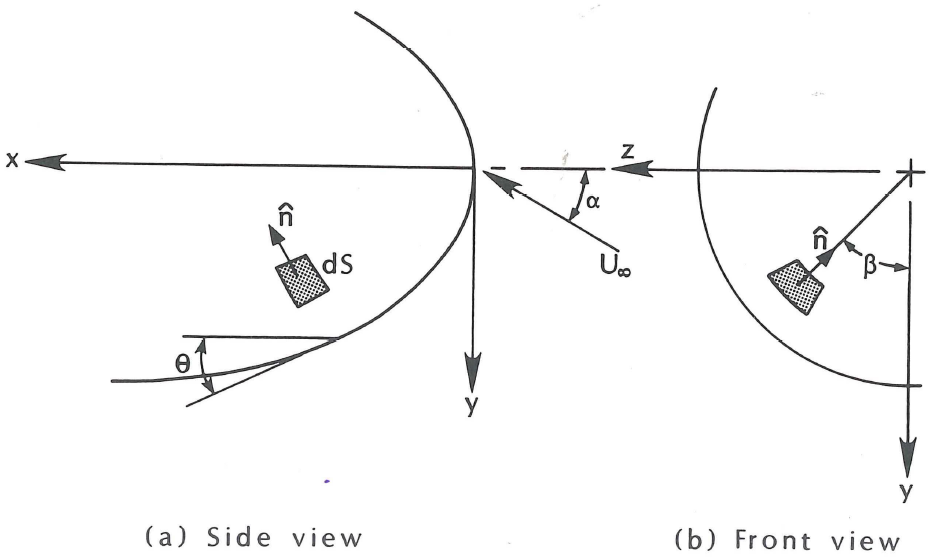
\includegraphics[width=0.7\textwidth]{./Figure/def_beta}
	\caption{Definition of \gls{sym:beta_cone} \cite{Bertin1994}}
	\label{fig:beta_cone}
\end{figure}

\begin{figure}[h]
	\centering
	\begin{subfigure}[b]{0.49\textwidth}
		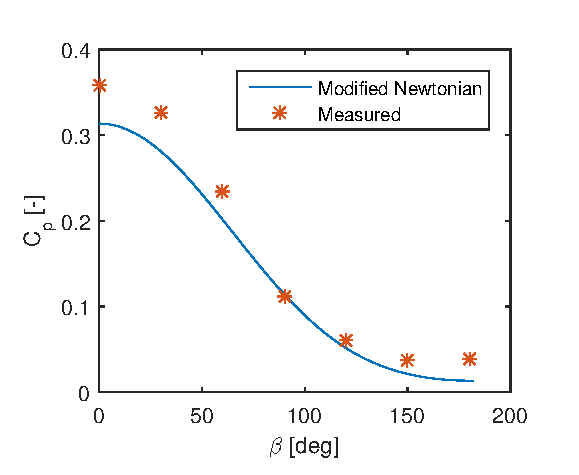
\includegraphics[width=0.96\textwidth]{./Figure/cone30deg_alpha10}
		\caption{$\gls{sym:alpha}=10\deg$}
		\label{fig:CPconealpha10}
	\end{subfigure}
		\begin{subfigure}[b]{0.49\textwidth}
			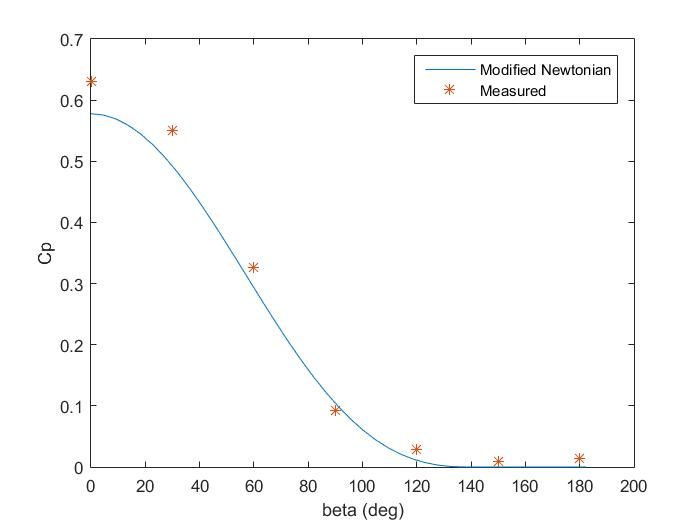
\includegraphics[width=0.96\textwidth]{./Figure/cone30deg_alpha20}
		\caption{$\gls{sym:alpha}=20\deg$}
		\label{fig:CPconealpha20}
	\end{subfigure}
	\caption{Comparisons between experimental and numerical \glspl{sym:CP}}
	\label{fig:CPcone30val}
\end{figure}

\subsubsection{\gls{sym:CD}-validation against experimental data of a sharp cone}
\label{subsubsec:valsharpconeCD}
Stevens found that for a sharp cone-cylinder with a half-cone angle \gls{sym:theta} of $30\deg$ $\gls{sym:CD}=0.58$ in an air-stream of Mach $8$ where angle of attack \gls{sym:alpha} and sideslip angle \gls{sym:beta} are zero \cite{Stevens1950,AndersonJr.2007}. The numerical model predicts for this case that $\gls{sym:CD}=0.456$, which coincides with a discrepancy of $21.4\%$ of the experimental value. This is in line with the results of Figure \ref{fig:CPcone30val} where the \glspl{sym:CP} predicted by the numerical model were smaller than the experimental values of a sharp cone.

\subsubsection{\gls{sym:CP}-validation against experimental data of the Apollo re-entry capsule}
\label{subsubsec:Apollo_validation}
The data points in Figure \ref{fig:Apollo_cp} represent pressure coefficients measured at various locations of one of the two axisymmetric axes \cite{Bertin1966}. The quantity shown on the X-axis is defined in Figure \ref{fig:Apollo_y}. As can be seen in Figure \ref{fig:Apollo_cp} the numerical model is most accurate around the centre of the capsule. As the distance to the centreline increases, so does the discrepancy between the experimental and numerical values.

\begin{figure}[H]
	\centering
	\setlength\figureheight{0.4\textwidth} 
	\setlength\figurewidth{0.95\textwidth}
	% This file was created by matlab2tikz.
% Minimal pgfplots version: 1.3
%
\definecolor{mycolor1}{rgb}{0.20810,0.16630,0.52920}%
\definecolor{mycolor2}{rgb}{0.19855,0.72140,0.63095}%
%
\begin{tikzpicture}

\begin{axis}[%
width=0.95092\figurewidth,
height=\figureheight,
at={(0\figurewidth,0\figureheight)},
scale only axis,
unbounded coords=jump,
xmin=-1.5,
xmax=1.5,
xlabel={$\frac{s}{R}$ [-]},
xmajorgrids,
ymin=0,
ymax=1.8,
ylabel={$C_p$ [-]},
ymajorgrids,
legend style={at={(0.5,0.03)},anchor=south,legend cell align=left,align=left,draw=white!15!black}
]
\addplot [color=mycolor1,solid]
  table[row sep=crcr]{%
-1.095	0.00194223338446491\\
-1.09496992147514	0\\
-1.09472939221993	0.0105764109659139\\
-1.09463923908848	0\\
-1.09415883985204	0.0286612804702033\\
-1.09400885921748	0\\
-1.09328990674072	0.0560242775566994\\
-1.09308050968954	0\\
-1.09212497457122	0.092367937353207\\
-1.09185673504618	0\\
-1.09066723634165	0.137297047773714\\
-1.09034088956864	0\\
-1.08892068761116	0.190322850013229\\
-1.08853712808401	0\\
-1.08689011554844	0.250868241388263\\
-1.08645039457714	nan\\
-1.08458108581034	0.318273930108563\\
-1.0819999272869	0.3918054818373\\
-1.07915371475421	0.470661188513422\\
-1.07605024948299	0.55398068095838\\
-1.07269803785581	0.640854198362098\\
-1.06910626805175	0.730332419944821\\
-1.06528478486218	0.821436757031353\\
-1.06124406270688	0.913169997566455\\
-1.05699517692443	1.00452718986455\\
-1.05254977341541	1.09450664823589\\
-1.04792003672184	1.18212096017887\\
-1.0431186566302	1.26640787317747\\
-1.03815879338958	1.34644093888065\\
-1.03305404164036	1.42133979364298\\
-1.02781839315226	1.42835417521564\\
-1.01832656548985	1.44935521736688\\
-0.986104624404206	1.50751538767456\\
-0.953709183690762	1.52351962805163\\
-0.921145943147255	1.5390688207566\\
-0.888420632094868	1.55415195599687\\
-0.855539008370191	1.56875835245074\\
-0.822506857312158	1.58287766497233\\
-0.789329990744154	1.59649989205813\\
-0.75601424595145	1.60961538306931\\
-0.72256548465417	1.62221484520418\\
-0.688989591975953	1.63428935021542\\
-0.655292475408497	1.64583034086682\\
-0.621480063772172	1.6568296371244\\
-0.587558306172872	1.66727944207735\\
-0.553533170955306	1.67717234758383\\
-0.519410644652901	1.68650133963741\\
-0.485196730934503	1.69525980344988\\
-0.450897449548067	1.7034415282464\\
-0.416518835261513	1.71104071176934\\
-0.382066936800948	1.71805196448708\\
-0.347547815786417	1.72447031350459\\
-0.312967545665402	1.7302912061727\\
-0.27833221064423	1.73551051339311\\
-0.243647904617593	1.74012453261658\\
-0.208920730096357	1.74412999053202\\
-0.174156797133862	1.74752404544416\\
-0.139362222250891	1.7503042893381\\
-0.104543127359504	1.75246874962895\\
-0.0697056386859186	1.75401589059533\\
-0.0348558856926369	1.75488268492153\\
-0	1.75525426236477\\
0.0348558856926369	1.75488268492153\\
0.0697056386859186	1.75401589059533\\
0.104543127359504	1.75246874962895\\
0.139362222250891	1.7503042893381\\
0.174156797133862	1.74752404544416\\
0.208920730096357	1.74412999053202\\
0.243647904617593	1.74012453261658\\
0.27833221064423	1.73551051339311\\
0.312967545665402	1.7302912061727\\
0.347547815786417	1.72447031350459\\
0.382066936800948	1.71805196448708\\
0.416518835261513	1.71104071176934\\
0.450897449548067	1.7034415282464\\
0.485196730934503	1.69525980344988\\
0.519410644652901	1.68650133963741\\
0.553533170955306	1.67717234758383\\
0.587558306172872	1.66727944207735\\
0.621480063772172	1.6568296371244\\
0.655292475408497	1.64583034086682\\
0.688989591975953	1.63428935021542\\
0.72256548465417	1.62221484520418\\
0.75601424595145	1.60961538306931\\
0.789329990744154	1.59649989205813\\
0.822506857312158	1.58287766497233\\
0.855539008370191	1.56875835245074\\
0.888420632094868	1.55415195599687\\
0.921145943147255	1.5390688207566\\
0.953709183690762	1.52351962805163\\
0.986104624404206	1.50751538767456\\
1.01832656548985	1.44935521736688\\
1.02781839315226	1.42835417521564\\
1.03305404164036	1.42133979364298\\
1.03815879338958	1.34644093888065\\
1.0431186566302	1.26640787317747\\
1.04792003672184	1.18212096017886\\
1.05254977341541	1.09450664823589\\
1.05699517692443	1.00452718986455\\
1.06124406270688	0.913169997566455\\
1.06528478486218	0.821436757031353\\
1.06910626805175	0.730332419944821\\
1.07269803785581	0.640854198362098\\
1.07605024948299	0.55398068095838\\
1.07915371475421	0.470661188513422\\
1.0819999272869	0.3918054818373\\
1.08458108581034	0.318273930108563\\
1.08645039457714	nan\\
1.08689011554844	0.250868241388263\\
1.08853712808401	0\\
1.08892068761116	0.190322850013229\\
1.09034088956864	0\\
1.09066723634165	0.137297047773714\\
1.09185673504618	0\\
1.09212497457122	0.0923679373532069\\
1.09308050968954	0\\
1.09328990674072	0.0560242775566994\\
1.09400885921748	0\\
1.09415883985204	0.0286612804702033\\
1.09463923908848	0\\
1.09472939221993	0.0105764109659139\\
1.09496992147514	0\\
1.095	0.0019422333844649\\
};
\addlegendentry{Modified Newtonian};

\addplot [color=mycolor2,only marks,mark=asterisk,mark options={solid}]
  table[row sep=crcr]{%
-1.02718093698553	0.326751322056051\\
-0.951551131339198	1.02168543257076\\
-0.799264139197169	1.4880212545932\\
-0.247616441864002	1.7300201625693\\
0.0180691662280614	1.74873159897289\\
0.273850147488554	1.70299372722051\\
0.547682381293604	1.63105638244619\\
0.68183629061674	1.49350323432687\\
0.817930550476365	1.44043342939967\\
0.871460439771112	1.37207156639853\\
0.929404854806911	1.26182928317321\\
0.981710021888355	0.939565894363321\\
1.0408671541418	0.31807000221393\\
1.09530512997895	0.0391870122023066\\
};
\addlegendentry{Measured};

\end{axis}
\end{tikzpicture}%
	\caption{Comparison between experimental and numerical \glspl{sym:CP} for the Apollo re-entry capsule}
	\label{fig:Apollo_cp}
\end{figure}

\begin{figure}[H]
	\centering
	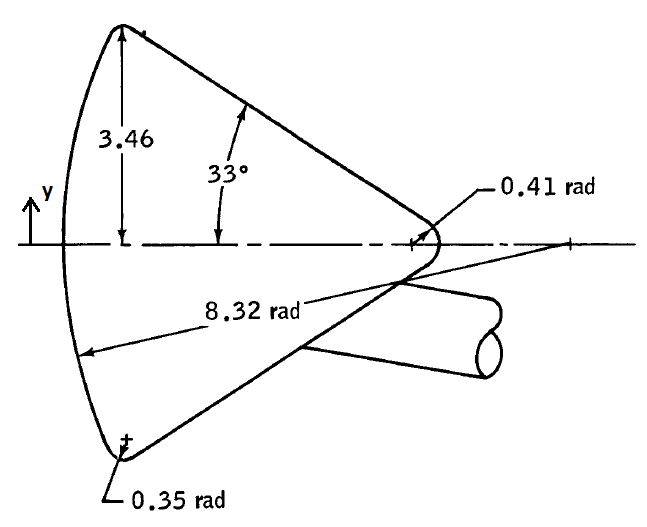
\includegraphics[width=0.4\textwidth]{./Figure/Apollo_model}
	\caption{Definition of unit on the horizontal axis of Figure \ref{fig:Apollo_cp} \cite{Bertin1966}}
	\label{fig:Apollo_y}
\end{figure}

\subsubsection{Maximum heat flux validation against experimental data of the \gls{irve} 3 vehicle}
\label{subsubsec:heatvalidation}
Dillman et al. observed that the maximum heat flux on the \acrfull{irve} 3 was $14.4$ $\frac{W}{cm^{2}}$ during re-entry at an altitude of $50$ kilometres and Mach $7.0$ \cite{Dillman2012}. The maximum heat flux computed by the numerical tool in the stagnation point for these flow conditions is $11.7$ $\frac{W}{cm^{2}}$. This is equal to $81.0\%$ of the experimental value. Thus a discrepancy of $19.0\%$ is present between the experimental and numerical maximum heat fluxes.

\subsubsection{Conclusions after the validation procedure}
\label{subsec:validconclusions}
From section \ref{subsec:aeroverval} it can be seen that the accuracy of the modified Newtonian method varies between geometries. The \gls{sym:CD} predicted in section \ref{subsubsec:valsphere} is accurate to within $1\%$ of the experimental value, whereas the accuracy of the \glspl{sym:CP} in section \ref{subsubsec:valsharpconeCP} varied over the cone surface. This discrepancy was also seen in section \ref{subsubsec:valsharpconeCD}, where the difference between the numerical and experimental \gls{sym:CD} was $21.4\%$, and again for the Apollo capsule in section \ref{subsubsec:Apollo_validation}. After judging the accuracy shown in Figures \ref{fig:CPcone30val} and \ref{fig:Apollo_cp} it was determined that the accuracy of the modified Newtonian method is adequate for the conceptual and preliminary design phases.
The model for the maximum heat flux found on a body was validated in section \ref{subsubsec:heatvalidation}. It was observed that a discrepancy of $19.0\%$ was present between the numerical and experimental maximum heat fluxes. After consideration this was deemed to be acceptable for conceptual and preliminary design.

\subsection{Application of analysis tool to system concepts}
\label{subsec:appaeroanal}
After the model development and validation, the different system concepts are evaluated on performance in the different trade-off criteria. Specifically, the lift, moment and aerodynamic heating are discussed. They are all related to the trade-off criteria as defined in Chapter \ref{ch:tradeoff}. Firstly, the relation between the aerodynamic properties and the trade-off criteria is discussed. After that, the results from the aerodynamic analysis is given.

The stability trade-off criterium is given by the static stability of the vehicle. This is characterised by the pitch moment gradient \gls{sym:cma-alpha}: if a positive angle of attack leads to a negative moment, the angle of attack is restored by the induced moment. This leads to a spacecraft that is less reactant to disturbances in the atmosphere, which leads to a less strict requirement on the control system keep the spacecraft pointed in the desired direction. A positive value of \gls{sym:cma-alpha} means the spacecraft is not stable, and the control system will have to very actively monitor the spacecraft in order for it to not diverge from the nominal condition.

Aerodynamic drag is used as the method to decelerate the vehicle from over escape velocity to $\gls{sym:M}=5$ before landing. The drag Equation is given in Eq. \ref{eq:drag}.
\begin{equation} \label{eq:drag}
\gls{sym:D} = \frac{1}{2}\gls{sym:rho}\gls{sym:V}^2\gls{sym:cda}
\end{equation}
As can be seen, the drag is dependent on the drag coefficient of the spacecraft as well as the density. In this sense, the maximum deceleration limit can be achieved by having the lowest part of an orbit lower if the drag coefficient is lower as well. Then, the higher density compensates for the low drag coefficient to produce the same force as a spacecraft with a high drag coefficient. In this way, the drag coefficient is not a key driver for the design. However, the spacecraft can influence its time in the atmosphere by producing lift: if the spacecraft were to fly out of the atmosphere, a downward pointing lift would divert it's trajectory more through the atmosphere. The spacecraft's ability to influence this trajectory through the atmosphere is thus characterised by the amount of lift that can be produced. This is characterised by the lift coefficient times the area of the spacecraft \gls{sym:cla}.

\subsubsection{Trade-off criteria justification} \label{sec:tradeoffaero}
In this section, the quantification method of the trade-off criteria relating to aerodynamics is justified.

The stability trade-off criterion is given by the static stability of the vehicle. This is characterised by the pitch moment gradient \gls{sym:cma-alpha}: For a negative \gls{sym:cma-alpha}, a positive angle of attack leads to a negative moment, such that the angle of attack is restored by the induced moment. This leads to a spacecraft that is less reactant to disturbances in the atmosphere, which leads to a less strict requirement on the control system to keep the spacecraft pointed in the desired direction. A positive value of \gls{sym:cma-alpha} means the spacecraft is not stable, and the control system will have to very actively monitor the spacecraft in order for it to not diverge from the required attitude. \\


Aerodynamic drag is used as the method to decelerate the vehicle from the initial velocity to $\gls{sym:M}=5$ before landing. The drag equation is given in Eq. \ref{eq:drag}.

\begin{equation} \label{eq:drag}
\gls{sym:D} = \frac{1}{2}\gls{sym:rho}\gls{sym:V}^2\gls{sym:cda}
\end{equation}
\begin{equation} \label{eq:lift}
\gls{sym:L} = \frac{1}{2}\gls{sym:rho}\gls{sym:V}^2\gls{sym:cla}
\end{equation}

The lift is defined as the component of the aerodynamic force perpendicular to the flow, where the direction away from Mars is defined positive. The drag component is defined parallel to the flow. For blunt bodies in hypersonic flow with the blunt side pointed towards the oncoming flow, a positive angle of attack results in a negative lift.

The drag and lift are dependent on the drag and lift coefficients of the spacecraft as well as the density. As can be seen in Figure \ref{fig:atmos_height_rho}, the density is significantly higher in lower parts of the atmosphere. For a given \gls{sym:cda}, the maximum deceleration can be chosen by varying the lowest part of the orbit: a higher density compensates for a low drag coefficient to produce the same force as a spacecraft with a high drag coefficient and a low density. Because of the large variation of density in the atmosphere, it is possible to find a trajectory for any \gls{sym:cda}. Thus, the drag coefficient itself is not a key driver for the design. However, the spacecraft can influence its deceleration time in the atmosphere by producing lift: if the spacecraft were to fly out of the atmosphere, a downward pointing lift would divert it's trajectory more through the atmosphere. The ability of the spacecraft to influence this trajectory through the atmosphere is characterised by the amount of lift that can be produced, with respect to the amount of drag produced at the same \gls{sym:alpha}. The dependence on drag is due to the fact that two spacecraft with the same \gls{sym:clcd} but a different \gls{sym:cda}, will just have the lowest part of the trajectory in a different height, where the total lift and drag force will be the same for both spacecraft. Therefore, the deceleration time is characterised by \gls{sym:clcd}. \\

The mass of the decelerator is composed of the structural mass, the \gls{tps} mass and the control system mass. 
The \gls{tps} mass is estimated based on the heat load on the spacecraft, which is the integral of the heat flux over time. This heat load is the total amount of heat supplied to the spacecraft between initial entry and final descent, and estimates the total amount of energy the \gls{tps} has to withstand. This can thus be used to size the thickness of the \gls{tps}, which leads directly to the mass of the system.
The control system mass is based on the moment that the control system has to provide. The amount of lift that a spacecraft has to produce in order to attain a desirable orbit directly dictates the angle of attack. This angle of attack, in turn, determines the moment that the control system has to compensate in order to maintain the required angle of attack. It is thus not the moment coefficient itself that has to be minimised, but rather the amount of moment that is needed to provide a certain amount of lift. Therefore, the ratio \gls{sym:cmcl} is used to quantify the control system mass.

In order to assess these values, a representative geometry is chosen. Since Newtonian flow only affects the parts of the vehicle that are in direct line of sight of the oncoming flow, only the front of the decelerator has to be accurately modelled. The stacked toroid and tension cone concepts are modelled after the \gls{irve} missions as flown by NASA, as can be seen in Figure \ref{fig:cpstackedtoroid}. The isotensoid model is modelled as a slightly flattened sphere, with a radius of 6 meters perpendicular and a radius of 5 meter in direction of the flow. This model can be seen in Figure \ref{fig:cpisotensoid}. The Trailing ballute is modelled as a single torus trailing body comparable to the rigid concept., as seen in Figure \ref{fig:cpballute}, and the rigid concept's front is a largely flattened sphere, as seen in Figure \ref{fig:cprigid}.


\begin{figure}[h]
	\centering
	\begin{subfigure}[b]{0.49\textwidth}
		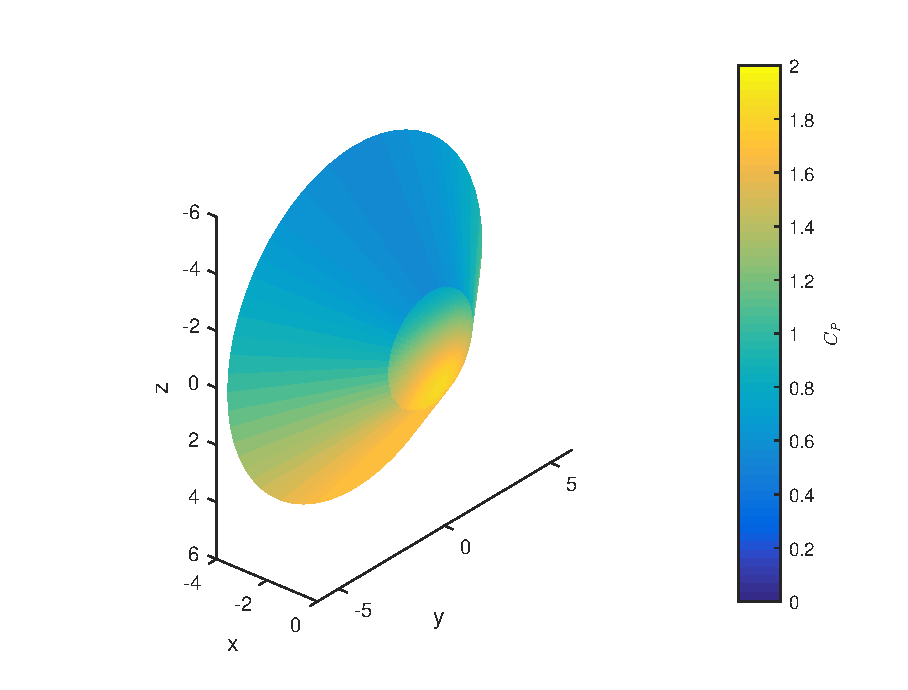
\includegraphics[width=0.96\textwidth]{./Figure/aero_model/irve.eps}
		\caption{Stacked toroid, tension cone}
		\label{fig:cpstackedtoroid}
	\end{subfigure}
	\begin{subfigure}[b]{0.49\textwidth}
		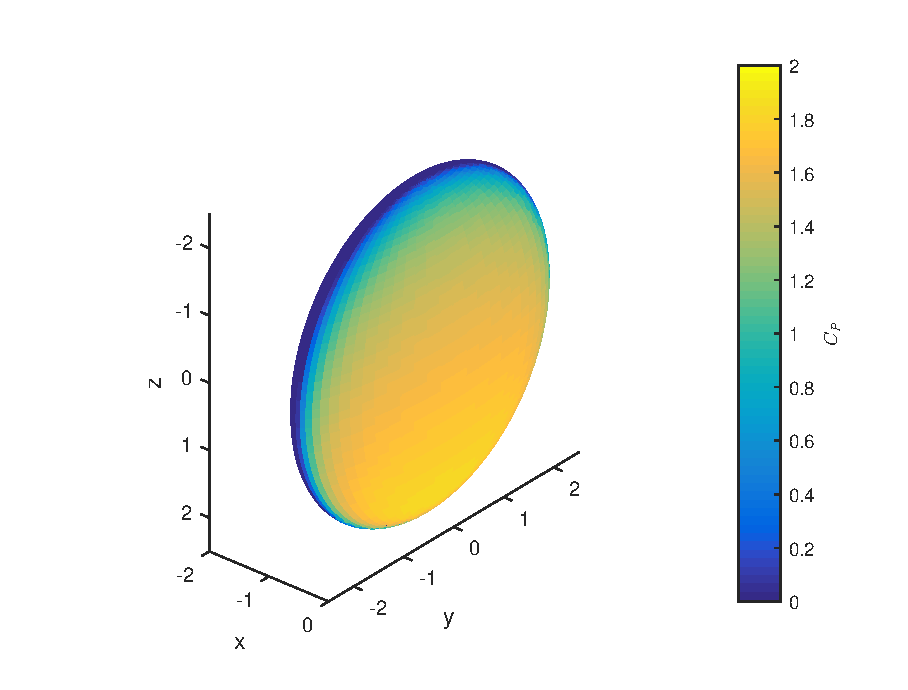
\includegraphics[width=0.96\textwidth]{./Figure/aero_model/rigid.eps}
		\caption{Rigid structure}
		\label{fig:cprigid}
	\end{subfigure}
	\begin{subfigure}[b]{0.49\textwidth}
		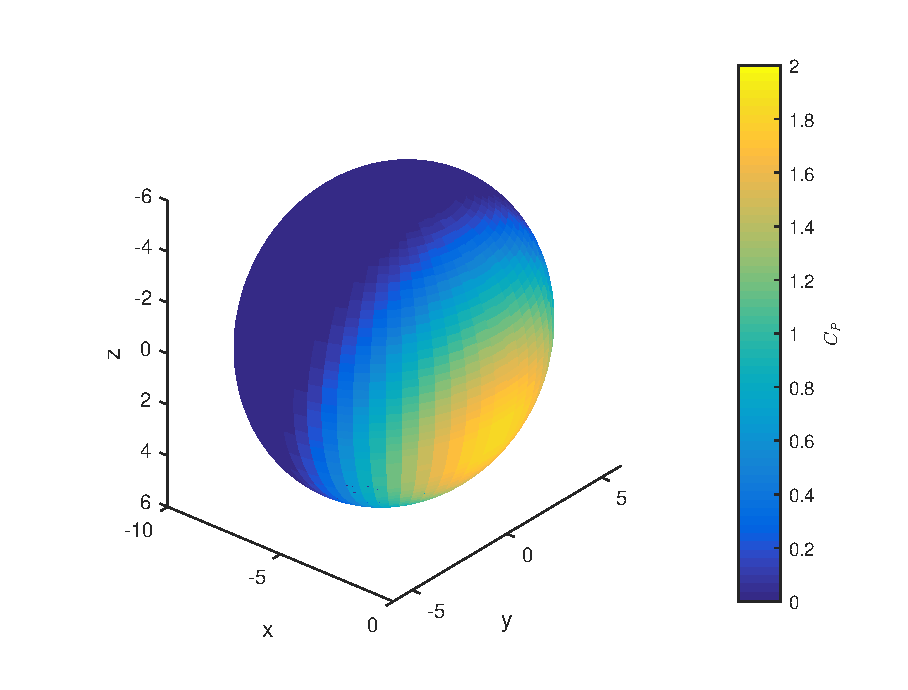
\includegraphics[width=0.96\textwidth]{./Figure/aero_model/isotensoid.eps}
		\caption{Isotensoid}
		\label{fig:cpisotensoid}
	\end{subfigure}
	\begin{subfigure}[b]{0.49\textwidth}
		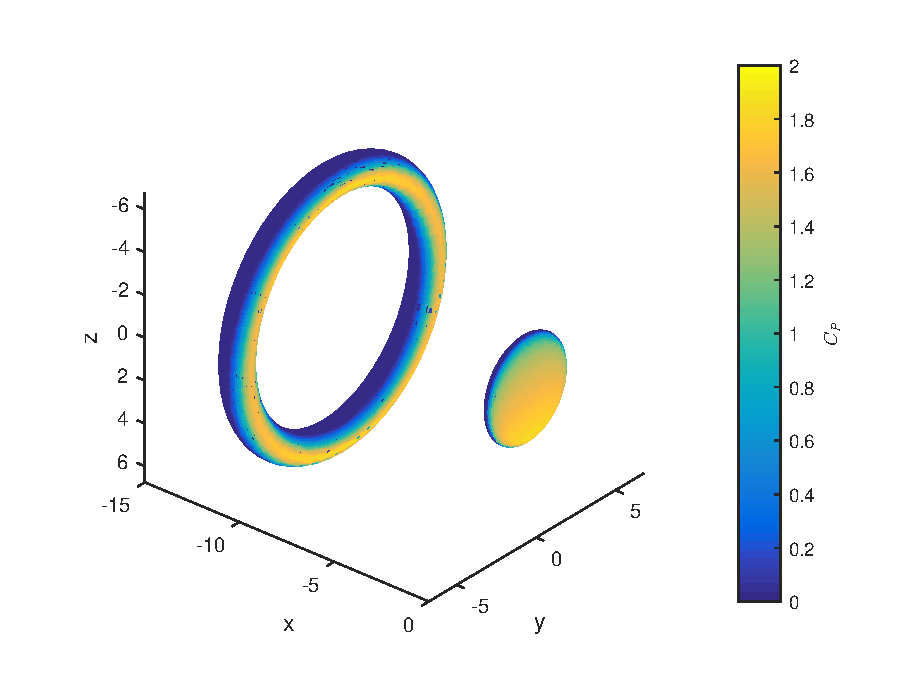
\includegraphics[width=0.96\textwidth]{./Figure/aero_model/ballute.eps}
		\caption{Trailing ballute}
		\label{fig:cpballute}
	\end{subfigure}	
	\caption{Geometry and pressure coefficient \gls{sym:CP} distribution over the different concepts, at an angle of attack $\gls{sym:alpha}=20[deg]$. }
	\label{fig:conceptscp}
\end{figure}

\subsubsection{Lift performance}
The lift is defined as the component of the aerodynamic force perpendicular to the flow, where the direction away from Mars is defined positive. The Equation used to calculate the total lift of a vehicle is given in Eq \ref{eq:lift}.
\begin{equation}
\gls{sym:L} = \frac{1}{2}\gls{sym:rho}\gls{sym:V}^2\gls{sym:cla}
\label{eq:lift}
\end{equation}
This $\gls{sym:cla}$ is the lift coefficient multiplied with the reference area and as such gives insight in the lift generation of a given spacecraft, incorporating its size. For blunt vehicles with a blunt surface perpendicular to the flow, a positive angle of attack $\gls{sym:alpha}$ results in a negative lift.

In Figure \ref{fig:clplots}, the lift coefficient can be seen to vary greatly for the different concepts: the stacked toroid and tension cone produce about 3 times the lift of the other concepts. This is also reflected in the lift gradient plot, which can be found in \ref{fig:claplha}. The lift gradient plot is the graph that provides the information needed for the trade-off, since the lift gradient determines how much the control system has to change the angle of attack to achieve a given lift. It is clear that the stacked toroid and tension cone have the greatest lift and lift gradient, while the trailing ballute follows closely. The other two concepts offer a significantly less lift performance. The lift and lift gradient at an angle of attack of $\gls{sym:alpha}=20^\circ$ are summarized in Table \ref{tab:clcdift}.

In order to assess these values, a representative geometry is chosen. Since Newtonian flow only affects the parts of the vehicle that are in direct line of sight of the oncoming flow, only the front of the decelerator has to be accurately modelled. The stacked toroid and tension cone concepts are modelled after the \gls{irve} missions as flown by NASA, as can be seen in Figure \ref{fig:cpstackedtoroid}. The rigid concept's front is a largely flattened sphere, as seen in Figure \ref{fig:cprigid}. The isotensoid is modelled as a slightly flattened sphere, with a radius of 6 meters perpendicular and a radius of 5 meter in direction of the flow. This model can be seen in Figure \ref{fig:cpisotensoid}. The trailing ballute is modelled as a single torus trailing a body comparable to the rigid concept, as seen in Figure \ref{fig:cpballute}, and 



\subsubsection{Deceleration performance}
$\gls{sym:clcd}$ is the lift coefficient divided by the drag coefficient. In Figure \ref{fig:clcd}, a graph is presented showing the lift over drag ratios of the different concepts for different angles of attack.


\begin{figure}[h]
	\centering
	\begin{subfigure}{0.49\textwidth}
		\setlength\figureheight{0.8\textwidth} 
		\setlength\figurewidth{0.75\textwidth}
		% This file was created by matlab2tikz.
% Minimal pgfplots version: 1.3
%
\definecolor{mycolor1}{rgb}{0.00000,0.44700,0.74100}%
\definecolor{mycolor2}{rgb}{0.85000,0.32500,0.09800}%
\definecolor{mycolor3}{rgb}{0.92900,0.69400,0.12500}%
\definecolor{mycolor4}{rgb}{0.49400,0.18400,0.55600}%
%
\begin{tikzpicture}

\begin{axis}[%
width=\figurewidth,
height=0.802158\figureheight,
at={(0\figurewidth,0\figureheight)},
scale only axis,
xmin=0,
xmax=60,
xlabel={$\alpha [deg]$},
xmajorgrids,
ymin=-1.2,
ymax=0.2,
ylabel={$\frac{C_L}{C_D} [-]$},
ymajorgrids,
axis x line*=bottom,
axis y line*=left,
legend style={at={(0.5,1.03)},anchor=south,legend cell align=left,align=left,draw=white!15!black}
]
\addplot [color=mycolor1,solid]
  table[row sep=crcr]{%
0	5.0364332293734e-17\\
1.01694915254237	-0.00886881038686472\\
2.03389830508475	-0.0177382765063238\\
3.05084745762712	-0.0266105083780653\\
4.06779661016949	-0.0354886933600949\\
5.08474576271186	-0.0443715105173429\\
6.10169491525424	-0.0532604572812532\\
7.11864406779661	-0.0621615184206523\\
8.13559322033898	-0.0710632131161607\\
9.15254237288135	-0.0799833143202747\\
10.1694915254237	-0.0889186009161462\\
11.1864406779661	-0.0978673650802531\\
12.2033898305085	-0.106836247271851\\
13.2203389830508	-0.115822465346637\\
14.2372881355932	-0.124823767028197\\
15.2542372881356	-0.13385762066535\\
16.271186440678	-0.14291508431104\\
17.2881355932203	-0.151998683525364\\
18.3050847457627	-0.161112597537135\\
19.3220338983051	-0.170258068271788\\
20.3389830508475	-0.179437846131841\\
21.3559322033898	-0.18866733028304\\
22.3728813559322	-0.197935572390311\\
23.3898305084746	-0.207246231336731\\
24.4067796610169	-0.216610676843288\\
25.4237288135593	-0.226029079788545\\
26.4406779661017	-0.235500402027576\\
27.4576271186441	-0.245048797158496\\
28.4745762711864	-0.254675524395709\\
29.4915254237288	-0.264368970690935\\
30.5084745762712	-0.274144565505753\\
31.5254237288136	-0.284000869710777\\
32.5423728813559	-0.293963000520449\\
33.5593220338983	-0.304046514060793\\
34.5762711864407	-0.314230454783092\\
35.593220338983	-0.324548428710094\\
36.6101694915254	-0.334995581514627\\
37.6271186440678	-0.345581250359487\\
38.6440677966102	-0.356350505539155\\
39.6610169491525	-0.367299029893162\\
40.6779661016949	-0.378437450608654\\
41.6949152542373	-0.389774409373945\\
42.7118644067797	-0.401343527185476\\
43.728813559322	-0.41316823288265\\
44.7457627118644	-0.425261011495103\\
45.7627118644068	-0.437653761709246\\
46.7796610169491	-0.450372618961619\\
47.7966101694915	-0.463449434162733\\
48.8135593220339	-0.476919208845705\\
49.8305084745763	-0.49082191311632\\
50.8474576271186	-0.505195519628189\\
51.864406779661	-0.52009645855347\\
52.8813559322034	-0.53556657562102\\
53.8983050847458	-0.551648196470665\\
54.9152542372881	-0.568283757276648\\
55.9322033898305	-0.585449875597817\\
56.9491525423729	-0.603102595782494\\
57.9661016949153	-0.621254764307888\\
58.9830508474576	-0.63997775013727\\
60	-0.659105608112932\\
};
\addlegendentry{Stacked Toroid, Tension Cone};

\addplot [color=mycolor2,solid]
  table[row sep=crcr]{%
0	-1.483383500215e-17\\
1.01694915254237	-0.0154466075973433\\
2.03389830508475	-0.0308983215205245\\
3.05084745762712	-0.0463610560478669\\
4.06779661016949	-0.0618446102232318\\
5.08474576271186	-0.0773505143140998\\
6.10169491525424	-0.0928846627742007\\
7.11864406779661	-0.108456004644763\\
8.13559322033898	-0.124060991440119\\
9.15254237288135	-0.139718543875477\\
10.1694915254237	-0.155430602443469\\
11.1864406779661	-0.171192864752111\\
12.2033898305085	-0.187025937831282\\
13.2203389830508	-0.202926542000502\\
14.2372881355932	-0.218894684168724\\
15.2542372881356	-0.234955117035483\\
16.271186440678	-0.251097330959081\\
17.2881355932203	-0.267325606621165\\
18.3050847457627	-0.283660857944599\\
19.3220338983051	-0.300097464002817\\
20.3389830508475	-0.316642583385728\\
21.3559322033898	-0.333303073436136\\
22.3728813559322	-0.350089018916926\\
23.3898305084746	-0.366999519799466\\
24.4067796610169	-0.384038482704838\\
25.4237288135593	-0.401209914092416\\
26.4406779661017	-0.418523695535869\\
27.4576271186441	-0.435985520643127\\
28.4745762711864	-0.45360606313891\\
29.4915254237288	-0.471391353616969\\
30.5084745762712	-0.4893223886892\\
31.5254237288136	-0.507417402286324\\
32.5423728813559	-0.525683568328429\\
33.5593220338983	-0.544103614941209\\
34.5762711864407	-0.56271670835948\\
35.593220338983	-0.581467260500827\\
36.6101694915254	-0.600388686064697\\
37.6271186440678	-0.619538178488193\\
38.6440677966102	-0.638815202222698\\
39.6610169491525	-0.65824500237328\\
40.6779661016949	-0.677841541292329\\
41.6949152542373	-0.697594877563252\\
42.7118644067797	-0.717460352349361\\
43.728813559322	-0.737481568527868\\
44.7457627118644	-0.757558996246075\\
45.7627118644068	-0.777789489185058\\
46.7796610169491	-0.798056114960774\\
47.7966101694915	-0.818317974641001\\
48.8135593220339	-0.838694944944911\\
49.8305084745763	-0.858950873214175\\
50.8474576271186	-0.879168337136622\\
51.864406779661	-0.899186236656746\\
52.8813559322034	-0.919089659008339\\
53.8983050847458	-0.938685318744582\\
54.9152542372881	-0.957937250327412\\
55.9322033898305	-0.976734437860176\\
56.9491525423729	-0.99497687539228\\
57.9661016949153	-1.01253569606119\\
58.9830508474576	-1.02934147729458\\
60	-1.04504382349516\\
};
\addlegendentry{Rigid};

\addplot [color=mycolor3,solid]
  table[row sep=crcr]{%
0	-1.90537580047186e-17\\
1.01694915254237	-0.00388449332173622\\
2.03389830508475	-0.0077711352640538\\
3.05084745762712	-0.0116588219579171\\
4.06779661016949	-0.0155409246522078\\
5.08474576271186	-0.0194088377935679\\
6.10169491525424	-0.0232625567357673\\
7.11864406779661	-0.0270974626647968\\
8.13559322033898	-0.0309045560337592\\
9.15254237288135	-0.0346868341158774\\
10.1694915254237	-0.0384345188395192\\
11.1864406779661	-0.0421445747251795\\
12.2033898305085	-0.0458169197904375\\
13.2203389830508	-0.0494502569125963\\
14.2372881355932	-0.0530371084378388\\
15.2542372881356	-0.056576648472266\\
16.271186440678	-0.0600592684285724\\
17.2881355932203	-0.0634864072750192\\
18.3050847457627	-0.0668559233344702\\
19.3220338983051	-0.0701641858629192\\
20.3389830508475	-0.0734106705211148\\
21.3559322033898	-0.0765839440703246\\
22.3728813559322	-0.0796808825502233\\
23.3898305084746	-0.0826986669147268\\
24.4067796610169	-0.0856394063459\\
25.4237288135593	-0.0884977329936396\\
26.4406779661017	-0.0912686931180848\\
27.4576271186441	-0.0939468736822213\\
28.4745762711864	-0.0965291977703355\\
29.4915254237288	-0.0990099320252114\\
30.5084745762712	-0.101393982347161\\
31.5254237288136	-0.103669318481619\\
32.5423728813559	-0.105841249157396\\
33.5593220338983	-0.107901939900376\\
34.5762711864407	-0.109841974772035\\
35.593220338983	-0.111651588839047\\
36.6101694915254	-0.113351717263537\\
37.6271186440678	-0.114927213048414\\
38.6440677966102	-0.11637293487655\\
39.6610169491525	-0.117677581483272\\
40.6779661016949	-0.118840943288529\\
41.6949152542373	-0.119880718640198\\
42.7118644067797	-0.120780216790739\\
43.728813559322	-0.121526977373284\\
44.7457627118644	-0.122123248053378\\
45.7627118644068	-0.122570601134165\\
46.7796610169491	-0.122871597151468\\
47.7966101694915	-0.123024818608255\\
48.8135593220339	-0.123010783232722\\
49.8305084745763	-0.122835509599402\\
50.8474576271186	-0.122501611583236\\
51.864406779661	-0.122011984834728\\
52.8813559322034	-0.121364823591745\\
53.8983050847458	-0.120548104510166\\
54.9152542372881	-0.119565153864216\\
55.9322033898305	-0.118403165245806\\
56.9491525423729	-0.117098457136955\\
57.9661016949153	-0.115630804835734\\
58.9830508474576	-0.113978607232654\\
60	-0.112175112033318\\
};
\addlegendentry{Isotensoid};

\addplot [color=mycolor4,solid]
  table[row sep=crcr]{%
0	-2.28022995225568e-17\\
1.01694915254237	-0.0109039532707526\\
2.03389830508475	-0.0218103459567605\\
3.05084745762712	-0.0327169986285077\\
4.06779661016949	-0.0436329837997838\\
5.08474576271186	-0.0545464969621898\\
6.10169491525424	-0.0654591033129618\\
7.11864406779661	-0.0763408429945217\\
8.13559322033898	-0.087179804352967\\
9.15254237288135	-0.0979914069080698\\
10.1694915254237	-0.108764158113581\\
11.1864406779661	-0.119498605569514\\
12.2033898305085	-0.130189386360552\\
13.2203389830508	-0.140848593828011\\
14.2372881355932	-0.151465879586014\\
15.2542372881356	-0.162041030492625\\
16.271186440678	-0.172558252582399\\
17.2881355932203	-0.183004895775267\\
18.3050847457627	-0.193378433979145\\
19.3220338983051	-0.203664649485995\\
20.3389830508475	-0.213851966443941\\
21.3559322033898	-0.223944370362439\\
22.3728813559322	-0.233935361308867\\
23.3898305084746	-0.243813793907642\\
24.4067796610169	-0.253579681430793\\
25.4237288135593	-0.263221820330201\\
26.4406779661017	-0.272722180985976\\
27.4576271186441	-0.282064785017106\\
28.4745762711864	-0.291231570106086\\
29.4915254237288	-0.300203697633695\\
30.5084745762712	-0.308977133971422\\
31.5254237288136	-0.317531899314625\\
32.5423728813559	-0.325854578170721\\
33.5593220338983	-0.333945089423567\\
34.5762711864407	-0.341779350568318\\
35.593220338983	-0.349334267939829\\
36.6101694915254	-0.356587058328937\\
37.6271186440678	-0.363513901990876\\
38.6440677966102	-0.370082642652605\\
39.6610169491525	-0.376273577369382\\
40.6779661016949	-0.382060152503511\\
41.6949152542373	-0.387433207627469\\
42.7118644067797	-0.392359995936341\\
43.728813559322	-0.396813802797211\\
44.7457627118644	-0.400796572157437\\
45.7627118644068	-0.404269589721614\\
46.7796610169491	-0.407179637342069\\
47.7966101694915	-0.409515230850841\\
48.8135593220339	-0.411232753212426\\
49.8305084745763	-0.412301337227769\\
50.8474576271186	-0.41271412549706\\
51.864406779661	-0.412450868135715\\
52.8813559322034	-0.411464637236779\\
53.8983050847458	-0.409780030027918\\
54.9152542372881	-0.407347046000251\\
55.9322033898305	-0.404176579593569\\
56.9491525423729	-0.400226031597585\\
57.9661016949153	-0.395504520581756\\
58.9830508474576	-0.389939336639685\\
60	-0.383624227094728\\
};
\addlegendentry{Trailing Ballute};

\end{axis}
\end{tikzpicture}%
		\caption{$\gls{sym:clcd}$}
		\label{fig:clcd}
	\end{subfigure}
	\begin{subfigure}{0.49\textwidth}
		\setlength\figureheight{0.8\textwidth} 
		\setlength\figurewidth{0.75\textwidth}
		% This file was created by matlab2tikz.
% Minimal pgfplots version: 1.3
%
\definecolor{mycolor1}{rgb}{0.00000,0.44700,0.74100}%
\definecolor{mycolor2}{rgb}{0.85000,0.32500,0.09800}%
\definecolor{mycolor3}{rgb}{0.92900,0.69400,0.12500}%
\definecolor{mycolor4}{rgb}{0.49400,0.18400,0.55600}%
%
\begin{tikzpicture}

\begin{axis}[%
width=\figurewidth,
height=0.802158\figureheight,
at={(0\figurewidth,0\figureheight)},
scale only axis,
xmin=0,
xmax=60,
xlabel={$\alpha [deg]$},
xmajorgrids,
ymin=-20,
ymax=15,
ylabel={$\frac{C_MA}{C_L} [-]$},
ymajorgrids,
axis x line*=bottom,
axis y line*=left,
legend style={at={(0.5,1.03)},anchor=south,legend cell align=left,align=left,draw=white!15!black}
]
\addplot [color=mycolor1,solid]
  table[row sep=crcr]{%
1.01694915254237	5.812432750332\\
2.03389830508475	5.81225204722886\\
3.05084745762712	5.81226937078523\\
4.06779661016949	5.81220741005694\\
5.08474576271186	5.812289824093\\
6.10169491525424	5.81220961388144\\
7.11864406779661	5.81205441545369\\
8.13559322033898	5.81190289799846\\
9.15254237288135	5.81182476020909\\
10.1694915254237	5.81144536654267\\
11.1864406779661	5.81096921817517\\
12.2033898305085	5.81071554572176\\
13.2203389830508	5.80996893365034\\
14.2372881355932	5.80914382993628\\
15.2542372881356	5.80836150643255\\
16.271186440678	5.80705837902709\\
17.2881355932203	5.80548872824994\\
18.3050847457627	5.80395637224526\\
19.3220338983051	5.80196025422491\\
20.3389830508475	5.79970432994437\\
21.3559322033898	5.79686197155915\\
22.3728813559322	5.79371772159237\\
23.3898305084746	5.79024431083639\\
24.4067796610169	5.78610405137767\\
25.4237288135593	5.78138471641395\\
26.4406779661017	5.77605627752874\\
27.4576271186441	5.76997277094465\\
28.4745762711864	5.76315788959835\\
29.4915254237288	5.75561212491598\\
30.5084745762712	5.74718701482204\\
31.5254237288136	5.73765824983282\\
32.5423728813559	5.72700487215989\\
33.5593220338983	5.71540447142333\\
34.5762711864407	5.70253650746238\\
35.593220338983	5.68842583820993\\
36.6101694915254	5.6729085512171\\
37.6271186440678	5.65585327510734\\
38.6440677966102	5.63722797379622\\
39.6610169491525	5.61679142277402\\
40.6779661016949	5.59453277654383\\
41.6949152542373	5.57041904185644\\
42.7118644067797	5.54436399256784\\
43.728813559322	5.51595041661538\\
44.7457627118644	5.48510771606048\\
45.7627118644068	5.45203126458758\\
46.7796610169491	5.41644200579519\\
47.7966101694915	5.37778334565652\\
48.8135593220339	5.3364017654927\\
49.8305084745763	5.29194808336269\\
50.8474576271186	5.24438896949017\\
51.864406779661	5.19341885828596\\
52.8813559322034	5.13892721977753\\
53.8983050847458	5.08098939583137\\
54.9152542372881	5.02162829608016\\
55.9322033898305	4.96136966317792\\
56.9491525423729	4.9013613052535\\
57.9661016949153	4.84188550140218\\
58.9830508474576	4.78323680984551\\
60	4.72566046517559\\
};
\addlegendentry{Stacked Toroid, Tension Cone};

\addplot [color=mycolor2,solid]
  table[row sep=crcr]{%
1.01694915254237	0.409731548404068\\
2.03389830508475	0.409897419264135\\
3.05084745762712	0.410179177623357\\
4.06779661016949	0.410547514239118\\
5.08474576271186	0.411006165829971\\
6.10169491525424	0.411618817094773\\
7.11864406779661	0.412292022659093\\
8.13559322033898	0.413099999183387\\
9.15254237288135	0.413993859098881\\
10.1694915254237	0.414983396530723\\
11.1864406779661	0.416095997903808\\
12.2033898305085	0.417320638473081\\
13.2203389830508	0.418644915479638\\
14.2372881355932	0.420079672333806\\
15.2542372881356	0.421622029262081\\
16.271186440678	0.423279702546655\\
17.2881355932203	0.425058532109178\\
18.3050847457627	0.426945086391907\\
19.3220338983051	0.428952131507732\\
20.3389830508475	0.431083060850429\\
21.3559322033898	0.433332217285695\\
22.3728813559322	0.435705525698678\\
23.3898305084746	0.438210296419583\\
24.4067796610169	0.44084559540629\\
25.4237288135593	0.443607464525025\\
26.4406779661017	0.44650683497495\\
27.4576271186441	0.449549959704081\\
28.4745762711864	0.452713968158553\\
29.4915254237288	0.45602225131753\\
30.5084745762712	0.459496992425321\\
31.5254237288136	0.463108753769268\\
32.5423728813559	0.466866604973851\\
33.5593220338983	0.470804261277417\\
34.5762711864407	0.474869465494047\\
35.593220338983	0.479113389156326\\
36.6101694915254	0.483529821039169\\
37.6271186440678	0.488070836685671\\
38.6440677966102	0.492820597118182\\
39.6610169491525	0.497738699898093\\
40.6779661016949	0.502821244643096\\
41.6949152542373	0.508078917466737\\
42.7118644067797	0.513529123897546\\
43.728813559322	0.519155273337902\\
44.7457627118644	0.524979990830867\\
45.7627118644068	0.530956353954562\\
46.7796610169491	0.537123657395333\\
47.7966101694915	0.543494280711557\\
48.8135593220339	0.5500164120533\\
49.8305084745763	0.556719870047816\\
50.8474576271186	0.563588641910174\\
51.864406779661	0.570617342919393\\
52.8813559322034	0.577793546412803\\
53.8983050847458	0.585090581730032\\
54.9152542372881	0.592506969330875\\
55.9322033898305	0.600026124810018\\
56.9491525423729	0.60758629680727\\
57.9661016949153	0.615166434873581\\
58.9830508474576	0.622754228291811\\
60	0.630228404932895\\
};
\addlegendentry{Rigid};

\addplot [color=mycolor3,solid]
  table[row sep=crcr]{%
1.01694915254237	-5.72198978784523\\
2.03389830508475	-5.71963042430175\\
3.05084745762712	-5.71931972711037\\
4.06779661016949	-5.72327367764864\\
5.08474576271186	-5.73223832764273\\
6.10169491525424	-5.74489359262982\\
7.11864406779661	-5.76138868981066\\
8.13559322033898	-5.78154699475065\\
9.15254237288135	-5.80502313037338\\
10.1694915254237	-5.83271127320292\\
11.1864406779661	-5.86432581095567\\
12.2033898305085	-5.89886931495406\\
13.2203389830508	-5.9366798786246\\
14.2372881355932	-5.97776826866406\\
15.2542372881356	-6.02225162727215\\
16.271186440678	-6.07046270638874\\
17.2881355932203	-6.12261670099767\\
18.3050847457627	-6.17839271975447\\
19.3220338983051	-6.2374816133866\\
20.3389830508475	-6.30038468856094\\
21.3559322033898	-6.36758155843215\\
22.3728813559322	-6.43918202590474\\
23.3898305084746	-6.51514385749122\\
24.4067796610169	-6.59541122901668\\
25.4237288135593	-6.68011654376085\\
26.4406779661017	-6.76974827566852\\
27.4576271186441	-6.86472855798566\\
28.4745762711864	-6.96487521847119\\
29.4915254237288	-7.07059976311547\\
30.5084745762712	-7.18210903550763\\
31.5254237288136	-7.29938076950136\\
32.5423728813559	-7.42256890001224\\
33.5593220338983	-7.55246509292594\\
34.5762711864407	-7.68991071674657\\
35.593220338983	-7.83516795911944\\
36.6101694915254	-7.9872739299621\\
37.6271186440678	-8.14694379995979\\
38.6440677966102	-8.31577295141286\\
39.6610169491525	-8.49436978290752\\
40.6779661016949	-8.68253070449979\\
41.6949152542373	-8.88008380662239\\
42.7118644067797	-9.08800247593833\\
43.728813559322	-9.30844677744136\\
44.7457627118644	-9.54149585583391\\
45.7627118644068	-9.78780758298434\\
46.7796610169491	-10.0471271419845\\
47.7966101694915	-10.3206394482787\\
48.8135593220339	-10.6120948494869\\
49.8305084745763	-10.920653176253\\
50.8474576271186	-11.2476939007541\\
51.864406779661	-11.5945399603172\\
52.8813559322034	-11.9620210017049\\
53.8983050847458	-12.3543798485846\\
54.9152542372881	-12.7722225735289\\
55.9322033898305	-13.2196918623462\\
56.9491525423729	-13.6942961850509\\
57.9661016949153	-14.2020973514666\\
58.9830508474576	-14.7493986647618\\
60	-15.3338401578997\\
};
\addlegendentry{Isotensoid};

\addplot [color=mycolor4,solid]
  table[row sep=crcr]{%
1.01694915254237	4.99475236453802\\
2.03389830508475	4.99552751452593\\
3.05084745762712	4.99709012778328\\
4.06779661016949	4.99906839115254\\
5.08474576271186	5.00192137901915\\
6.10169491525424	5.00819142867877\\
7.11864406779661	5.02035702534533\\
8.13559322033898	5.03776481581709\\
9.15254237288135	5.05920473160801\\
10.1694915254237	5.08402707937186\\
11.1864406779661	5.1112677655293\\
12.2033898305085	5.14129151020146\\
13.2203389830508	5.17300486906476\\
14.2372881355932	5.20658382950142\\
15.2542372881356	5.24224116704726\\
16.271186440678	5.28059419125194\\
17.2881355932203	5.32239115350643\\
18.3050847457627	5.36787747158082\\
19.3220338983051	5.41713538137331\\
20.3389830508475	5.47023265845462\\
21.3559322033898	5.52676760702964\\
22.3728813559322	5.58707304131202\\
23.3898305084746	5.65079614669661\\
24.4067796610169	5.7180135238723\\
25.4237288135593	5.78880261917195\\
26.4406779661017	5.86375454039584\\
27.4576271186441	5.94348507719536\\
28.4745762711864	6.02832358747471\\
29.4915254237288	6.1185035752032\\
30.5084745762712	6.21400898138649\\
31.5254237288136	6.31509952686487\\
32.5423728813559	6.422123323515\\
33.5593220338983	6.53487526384533\\
34.5762711864407	6.65374954182092\\
35.593220338983	6.77930575104886\\
36.6101694915254	6.91213892749494\\
37.6271186440678	7.05263680559825\\
38.6440677966102	7.20189354918909\\
39.6610169491525	7.36008827165392\\
40.6779661016949	7.52782127797161\\
41.6949152542373	7.70577217809486\\
42.7118644067797	7.89427355435284\\
43.728813559322	8.09430367988275\\
44.7457627118644	8.30598670896689\\
45.7627118644068	8.53036814353213\\
46.7796610169491	8.76917954597077\\
47.7966101694915	9.0231910801453\\
48.8135593220339	9.29446420748853\\
49.8305084745763	9.58442647576004\\
50.8474576271186	9.89350336787161\\
51.864406779661	10.2240327354255\\
52.8813559322034	10.5777906341913\\
53.8983050847458	10.9559666602201\\
54.9152542372881	11.3614238972067\\
55.9322033898305	11.7959127022701\\
56.9491525423729	12.2638923931838\\
57.9661016949153	12.7672317823524\\
58.9830508474576	13.3131153811816\\
60	13.9006629541795\\
};
\addlegendentry{Trailing Ballute};

\end{axis}
\end{tikzpicture}%	
		\caption{$\gls{sym:cmcl}$}
		\label{fig:cmcl}
	\end{subfigure}
	\caption{Comparisons of the different concepts for $\gls{sym:clcd}$ and $\gls{sym:cmcl}$. $\gls{sym:M}=20[-]$, $\gls{sym:gamma}=1.29[-]$}
	\label{fig:cmcl-clcd}
\end{figure}

The lift over drag ratio seems to be linear up until around $\gls{sym:alpha}=20 [deg]$. Furthermore, there is a clear distinction between the different concepts: at $\gls{sym:alpha}=20 [deg]$, the rigid concepts performs best, followed by the stacked toroid, tension con and trailing ballute. The isotensoid performs worst. The results are summarized in table \ref{tab:clcd}.

\begin{table}[H]
	\caption{Lift over drag ratio of the different concepts at $\gls{sym:alpha}=20 [deg]$. $\gls{sym:M}=20[-]$, $\gls{sym:gamma}=1.29[-]$}% CAPTION HERE !
	\label{tab:clcd}% LABEL HERE
	\begin{tabular}{|p{0.36\textwidth}|p{0.23\textwidth}|p{0.31\textwidth}|}
		\hline
		\textbf{Concept}  				& \textbf{$\gls{sym:clcd}$}	& \textbf{Fraction of stacked toroid}	\\ \hline \hline
		Stacked toroid, tension cone	& -0.176     				& 1								\\ \hline
		Rigid  							& -0.311					& 1.764						\\ \hline
		Isotensoid  					& -0.072					& 0.410						\\ \hline
		Trailing ballute				& -0.210					& 1.193						\\ \hline
	\end{tabular}
\end{table}

\begin{figure}[h]
	\centering
	\begin{subfigure}[b]{0.49\textwidth}
		\setlength\figureheight{0.8\textwidth} 
		\setlength\figurewidth{0.75\textwidth}
		% This file was created by matlab2tikz.
% Minimal pgfplots version: 1.3
%
\definecolor{mycolor1}{rgb}{0.00000,0.44700,0.74100}%
\definecolor{mycolor2}{rgb}{0.85000,0.32500,0.09800}%
\definecolor{mycolor3}{rgb}{0.92900,0.69400,0.12500}%
\definecolor{mycolor4}{rgb}{0.49400,0.18400,0.55600}%
%
\begin{tikzpicture}

\begin{axis}[%
width=\figurewidth,
height=0.802158\figureheight,
at={(0\figurewidth,0\figureheight)},
scale only axis,
xmin=0,
xmax=60,
xlabel={$\alpha [deg]$},
xmajorgrids,
ymin=-40,
ymax=10,
ylabel={$C_LA [m^2]$},
ymajorgrids,
axis x line*=bottom,
axis y line*=left,
legend style={at={(0.5,1.03)},anchor=south,legend cell align=left,align=left,draw=white!15!black}
]
\addplot [color=mycolor1,solid]
  table[row sep=crcr]{%
0	7.1054e-15\\
1.01694915254237	-1.25084347544066\\
2.03389830508475	-2.50011393183131\\
3.05084745762712	-3.7461823046288\\
4.06779661016949	-4.9875928829058\\
5.08474576271186	-6.22267531788222\\
6.10169491525424	-7.44992821405236\\
7.11864406779661	-8.66806175682926\\
8.13559322033898	-9.87472231353828\\
9.15254237288135	-11.0695683224084\\
10.1694915254237	-12.2510330428494\\
11.1864406779661	-13.4170315677366\\
12.2033898305085	-14.566197956621\\
13.2203389830508	-15.6982359329274\\
14.2372881355932	-16.8108407638054\\
15.2542372881356	-17.9032509356107\\
16.271186440678	-18.974271496548\\
17.2881355932203	-20.0219906051449\\
18.3050847457627	-21.0463543084308\\
19.3220338983051	-22.0461067570062\\
20.3389830508475	-23.0194806590219\\
21.3559322033898	-23.9666944745205\\
22.3728813559322	-24.8867424272918\\
23.3898305084746	-25.7781069522303\\
24.4067796610169	-26.6410510330387\\
25.4237288135593	-27.473806202547\\
26.4406779661017	-28.2760731655754\\
27.4576271186441	-29.0480341844058\\
28.4745762711864	-29.7893323452044\\
29.4915254237288	-30.4986156948003\\
30.5084745762712	-31.1760337282012\\
31.5254237288136	-31.8217110043282\\
32.5423728813559	-32.4353613082934\\
33.5593220338983	-33.0171175151611\\
34.5762711864407	-33.5666369739459\\
35.593220338983	-34.0835643965626\\
36.6101694915254	-34.568743195601\\
37.6271186440678	-35.0221102540577\\
38.6440677966102	-35.4441394065079\\
39.6610169491525	-35.8352328704323\\
40.6779661016949	-36.195976063827\\
41.6949152542373	-36.5259042981576\\
42.7118644067797	-36.8263154408468\\
43.728813559322	-37.0978217548215\\
44.7457627118644	-37.3410152043556\\
45.7627118644068	-37.5563638577909\\
46.7796610169491	-37.7446005891436\\
47.7966101694915	-37.9074692958891\\
48.8135593220339	-38.0447680729122\\
49.8305084745763	-38.1578893506131\\
50.8474576271186	-38.2480287461758\\
51.864406779661	-38.3154603875428\\
52.8813559322034	-38.3619084400715\\
53.8983050847458	-38.3867607943534\\
54.9152542372881	-38.3825928955832\\
55.9322033898305	-38.3456347750797\\
56.9491525423729	-38.2718220872641\\
57.9661016949153	-38.1598531007056\\
58.9830508474576	-38.0081686193158\\
60	-37.8170264470767\\
};
\addlegendentry{Stacked Toroid, Tension Cone};

\addplot [color=mycolor2,solid]
  table[row sep=crcr]{%
0	-4.8296e-16\\
1.01694915254237	-0.502699624103774\\
2.03389830508475	-1.00431385159256\\
3.05084745762712	-1.50383088819974\\
4.06779661016949	-2.00025272962543\\
5.08474576271186	-2.49254665473588\\
6.10169491525424	-2.9795651532031\\
7.11864406779661	-3.46043137729257\\
8.13559322033898	-3.93385276382294\\
9.15254237288135	-4.39939331235438\\
10.1694915254237	-4.85574005389889\\
11.1864406779661	-5.30182866764367\\
12.2033898305085	-5.73712465875042\\
13.2203389830508	-6.16058680719576\\
14.2372881355932	-6.57122100179732\\
15.2542372881356	-6.96851676667261\\
16.271186440678	-7.35149941647659\\
17.2881355932203	-7.71943126284704\\
18.3050847457627	-8.0718611205636\\
19.3220338983051	-8.40783269928786\\
20.3389830508475	-8.72682366746812\\
21.3559322033898	-9.02848820003078\\
22.3728813559322	-9.3121193323405\\
23.3898305084746	-9.57721998207147\\
24.4067796610169	-9.82351154480774\\
25.4237288135593	-10.0505935628691\\
26.4406779661017	-10.2580182913938\\
27.4576271186441	-10.4456311548945\\
28.4745762711864	-10.613550509827\\
29.4915254237288	-10.7613335077798\\
30.5084745762712	-10.888477540312\\
31.5254237288136	-10.9954326716379\\
32.5423728813559	-11.0822079107475\\
33.5593220338983	-11.1483236215932\\
34.5762711864407	-11.1948941271536\\
35.593220338983	-11.2210820095789\\
36.6101694915254	-11.2273897995794\\
37.6271186440678	-11.2150873391081\\
38.6440677966102	-11.1828875325401\\
39.6610169491525	-11.1319811744807\\
40.6779661016949	-11.0628138297878\\
41.6949152542373	-10.9757609805323\\
42.7118644067797	-10.8711147469984\\
43.728813559322	-10.7495988509735\\
44.7457627118644	-10.6115942732337\\
45.7627118644068	-10.4585364190254\\
46.7796610169491	-10.290198326451\\
47.7966101694915	-10.1072265732406\\
48.8135593220339	-9.91126653057559\\
49.8305084745763	-9.70227189665971\\
50.8474576271186	-9.48135057456782\\
51.864406779661	-9.24916280799865\\
52.8813559322034	-9.00668248639224\\
53.8983050847458	-8.75482338022132\\
54.9152542372881	-8.49426773784043\\
55.9322033898305	-8.22596242387361\\
56.9491525423729	-7.95110028308175\\
57.9661016949153	-7.67031234236708\\
58.9830508474576	-7.38366543834402\\
60	-7.09443990849888\\
};
\addlegendentry{Rigid};

\addplot [color=mycolor3,solid]
  table[row sep=crcr]{%
0	-2.2613e-15\\
1.01694915254237	-0.46097084545134\\
2.03389830508475	-0.921951692849517\\
3.05084745762712	-1.38244976030582\\
4.06779661016949	-1.8413387829285\\
5.08474576271186	-2.29759842199526\\
6.10169491525424	-2.75065143098769\\
7.11864406779661	-3.19966320455431\\
8.13559322033898	-3.64373734161363\\
9.15254237288135	-4.08251685481998\\
10.1694915254237	-4.51481074336239\\
11.1864406779661	-4.93983188145749\\
12.2033898305085	-5.3578770567874\\
13.2203389830508	-5.76796061709334\\
14.2372881355932	-6.1693694796901\\
15.2542372881356	-6.56196081642723\\
16.271186440678	-6.94463175306355\\
17.2881355932203	-7.31666216075441\\
18.3050847457627	-7.67826640325574\\
19.3220338983051	-8.0289941309416\\
20.3389830508475	-8.36815016025898\\
21.3559322033898	-8.69505480690135\\
22.3728813559322	-9.00909886851422\\
23.3898305084746	-9.31013876084651\\
24.4067796610169	-9.5981734772589\\
25.4237288135593	-9.87277848821488\\
26.4406779661017	-10.1332463018947\\
27.4576271186441	-10.3790901738236\\
28.4745762711864	-10.6103942720126\\
29.4915254237288	-10.8267286599619\\
30.5084745762712	-11.028123566953\\
31.5254237288136	-11.2144598980028\\
32.5423728813559	-11.3858379150145\\
33.5593220338983	-11.5416651562966\\
34.5762711864407	-11.6809009613149\\
35.593220338983	-11.8036087701175\\
36.6101694915254	-11.9116302424854\\
37.6271186440678	-12.0042934829376\\
38.6440677966102	-12.0804297501214\\
39.6610169491525	-12.1400356741522\\
40.6779661016949	-12.1830930851061\\
41.6949152542373	-12.2116784227168\\
42.7118644067797	-12.224695203926\\
43.728813559322	-12.2211676678047\\
44.7457627118644	-12.2018476306027\\
45.7627118644068	-12.1670154800192\\
46.7796610169491	-12.117445638908\\
47.7966101694915	-12.0534259772343\\
48.8135593220339	-11.9732847540092\\
49.8305084745763	-11.8782488069265\\
50.8474576271186	-11.7687863284784\\
51.864406779661	-11.6456725767022\\
52.8813559322034	-11.5091035383786\\
53.8983050847458	-11.3582673112267\\
54.9152542372881	-11.1938059971517\\
55.9322033898305	-11.0149578253617\\
56.9491525423729	-10.8255297375786\\
57.9661016949153	-10.6238461342895\\
58.9830508474576	-10.4080649819663\\
60	-10.1820312047519\\
};
\addlegendentry{Isotensoid};

\addplot [color=mycolor4,solid]
  table[row sep=crcr]{%
0	-2.3402e-15\\
1.01694915254237	-1.11883799619006\\
2.03389830508475	-2.23589323162406\\
3.05084745762712	-3.34921701092899\\
4.06779661016949	-4.45724229402952\\
5.08474576271186	-5.55789934068606\\
6.10169491525424	-6.64818173430035\\
7.11864406779661	-7.72417529808867\\
8.13559322033898	-8.78292970736892\\
9.15254237288135	-9.82346540579282\\
10.1694915254237	-10.8432196349996\\
11.1864406779661	-11.8411812605142\\
12.2033898305085	-12.8149927316626\\
13.2203389830508	-13.7644591835265\\
14.2372881355932	-14.6873158086148\\
15.2542372881356	-15.5821466503814\\
16.271186440678	-16.4463119842287\\
17.2881355932203	-17.2776395862772\\
18.3050847457627	-18.074876159846\\
19.3220338983051	-18.8361690394125\\
20.3389830508475	-19.5597619284554\\
21.3559322033898	-20.2453676594955\\
22.3728813559322	-20.8922010885035\\
23.3898305084746	-21.4992747484046\\
24.4067796610169	-22.0662313497505\\
25.4237288135593	-22.5923070624167\\
26.4406779661017	-23.0761101953887\\
27.4576271186441	-23.5166366293491\\
28.4745762711864	-23.9131486264937\\
29.4915254237288	-24.2647090593546\\
30.5084745762712	-24.5718885985016\\
31.5254237288136	-24.8345056581061\\
32.5423728813559	-25.0527308236285\\
33.5593220338983	-25.2275806089958\\
34.5762711864407	-25.3589538977381\\
35.593220338983	-25.4469210977027\\
36.6101694915254	-25.4914754113575\\
37.6271186440678	-25.4932222498691\\
38.6440677966102	-25.4519410723652\\
39.6610169491525	-25.3685391562527\\
40.6779661016949	-25.2437659574479\\
41.6949152542373	-25.0797763695833\\
42.7118644067797	-24.8767889964506\\
43.728813559322	-24.6359267434714\\
44.7457627118644	-24.3601885464674\\
45.7627118644068	-24.0502590854217\\
46.7796610169491	-23.7053776288669\\
47.7966101694915	-23.3286908093536\\
48.8135593220339	-22.9200509711678\\
49.8305084745763	-22.4809659231968\\
50.8474576271186	-22.0146551825953\\
51.864406779661	-21.5221481091924\\
52.8813559322034	-21.0046250856605\\
53.8983050847458	-20.4661480638173\\
54.9152542372881	-19.906754051704\\
55.9322033898305	-19.3294406928294\\
56.9491525423729	-18.7348632418239\\
57.9661016949153	-18.1256416109231\\
58.9830508474576	-17.4998768817327\\
60	-16.8660874572644\\
};
\addlegendentry{Trailing Ballute};

\end{axis}
\end{tikzpicture}%
		\caption{$\gls{sym:cla}$}
		\label{fig:cl}
	\end{subfigure}
	\begin{subfigure}[b]{0.49\textwidth}
		\setlength\figureheight{0.8\textwidth} 
		\setlength\figurewidth{0.75\textwidth}
		% This file was created by matlab2tikz.
% Minimal pgfplots version: 1.3
%
\definecolor{mycolor1}{rgb}{0.00000,0.44700,0.74100}%
\definecolor{mycolor2}{rgb}{0.85000,0.32500,0.09800}%
\definecolor{mycolor3}{rgb}{0.92900,0.69400,0.12500}%
\definecolor{mycolor4}{rgb}{0.49400,0.18400,0.55600}%
%
\begin{tikzpicture}

\begin{axis}[%
width=\figurewidth,
height=0.802158\figureheight,
at={(0\figurewidth,0\figureheight)},
scale only axis,
unbounded coords=jump,
xmin=0,
xmax=60,
xlabel={$\alpha [deg]$},
xmajorgrids,
ymin=-80,
ymax=40,
ylabel={$C_{L_\alpha}A [\frac{m^2}{rad}]$},
ymajorgrids,
axis x line*=bottom,
axis y line*=left,
legend style={at={(0.5,1.03)},anchor=south,legend cell align=left,align=left,draw=white!15!black}
]
\addplot [color=mycolor1,solid]
  table[row sep=crcr]{%
0	-70.474989973071\\
1.01694915254237	-70.3907413773347\\
2.03389830508475	-70.2171546439008\\
3.05084745762712	-69.9650489887125\\
4.06779661016949	-69.6212685498195\\
5.08474576271186	-69.1933081242122\\
6.10169491525424	-68.7048710601719\\
7.11864406779661	-68.0698739977091\\
8.13559322033898	-67.4269340974213\\
9.15254237288135	-66.7048710601721\\
10.1694915254237	-65.8648339060711\\
11.1864406779661	-64.9283667621779\\
12.2033898305085	-64.0114613180517\\
13.2203389830508	-62.9438717067584\\
14.2372881355932	-61.8338108882522\\
15.2542372881356	-60.6876790830945\\
16.271186440678	-59.3928980526918\\
17.2881355932203	-58.1088825214898\\
18.3050847457627	-56.7908309455589\\
19.3220338983051	-55.3264604810998\\
20.3389830508475	-53.8681948424067\\
21.3559322033898	-52.43553008596\\
22.3728813559322	-50.801832760596\\
23.3898305084746	-49.2836676217767\\
24.4067796610169	-47.6217765042978\\
25.4237288135593	-45.9335624284076\\
26.4406779661017	-44.2013196442879\\
27.4576271186441	-42.4853935738792\\
28.4745762711864	-40.6868185334876\\
29.4915254237288	-38.8325123072178\\
30.5084745762712	-37.0508384770542\\
31.5254237288136	-35.2090051763032\\
32.5423728813559	-33.3962283728795\\
33.5593220338983	-31.5625901131824\\
34.5762711864407	-29.7110232735399\\
35.593220338983	-27.8683863089285\\
36.6101694915254	-26.0748834507147\\
37.6271186440678	-24.2622799496544\\
38.6440677966102	-22.5009364903002\\
39.6610169491525	-20.7537273174346\\
40.6779661016949	-19.0124684689877\\
41.6949152542373	-17.2961580071117\\
42.7118644067797	-15.649085502676\\
43.728813559322	-14.0227025671656\\
44.7457627118644	-12.4313251565255\\
45.7627118644068	-10.8747282890569\\
46.7796610169491	-9.40764839064201\\
47.7966101694915	-7.95690099835582\\
48.8135593220339	-6.56052386760777\\
49.8305084745763	-5.24146281992728\\
50.8474576271186	-3.94549081093487\\
51.864406779661	-2.73528218925421\\
52.8813559322034	-1.5088296846713\\
53.8983050847458	0.105937285270841\\
54.9152542372881	1.96391903916435\\
55.9322033898305	4.05261283772731\\
56.9491525423729	6.22610577973362\\
57.9661016949153	8.48818000344096\\
58.9830508474576	10.7451773036964\\
60	nan\\
};
\addlegendentry{Stacked Toroid, Tension Cone};

\addplot [color=mycolor2,solid]
  table[row sep=crcr]{%
0	-28.3234973929983\\
1.01694915254237	-28.2651541193996\\
2.03389830508475	-28.1516071735518\\
3.05084745762712	-27.9837277258924\\
4.06779661016949	-27.7602704406119\\
5.08474576271186	-27.4722126733127\\
6.10169491525424	-27.1404011461318\\
7.11864406779661	-26.729667812142\\
8.13559322033898	-26.3037249283668\\
9.15254237288135	-25.8051575931232\\
10.1694915254237	-25.2405498281787\\
11.1864406779661	-24.6532951289399\\
12.2033898305085	-24.0114613180515\\
13.2203389830508	-23.3046964490264\\
14.2372881355932	-22.5787965616048\\
15.2542372881356	-21.7994269340974\\
16.271186440678	-20.967926689576\\
17.2881355932203	-20.1260744985674\\
18.3050847457627	-19.2263610315186\\
19.3220338983051	-18.2875143184422\\
20.3389830508475	-17.3409742120343\\
21.3559322033898	-16.355300859599\\
22.3728813559322	-15.3321878579611\\
23.3898305084746	-14.2979942693408\\
24.4067796610169	-13.243553008596\\
25.4237288135593	-12.1649484536082\\
26.4406779661017	-11.0343790693877\\
27.4576271186441	-9.91271320934608\\
28.4745762711864	-8.78328552578349\\
29.4915254237288	-7.60753924588151\\
30.5084745762712	-6.43483352448726\\
31.5254237288136	-5.30255291480497\\
32.5423728813559	-4.12475035055877\\
33.5593220338983	-2.97053154449696\\
34.5762711864407	-1.86386051970757\\
35.593220338983	-0.67518651315055\\
36.6101694915254	0.38698654135807\\
37.6271186440678	1.48808764561306\\
38.6440677966102	2.60381507192484\\
39.6610169491525	3.63057849934538\\
40.6779661016949	4.66651571371468\\
41.6949152542373	5.66861193778969\\
42.7118644067797	6.64505797718551\\
43.728813559322	7.58696667883321\\
44.7457627118644	8.46702840230158\\
45.7627118644068	9.32893954229552\\
46.7796610169491	10.175254818104\\
47.7966101694915	10.9320984592582\\
48.8135593220339	11.6715821678836\\
49.8305084745763	12.3635804373627\\
50.8474576271186	13.0094893935395\\
51.864406779661	13.6035512688126\\
52.8813559322034	14.1436492994352\\
53.8983050847458	14.6428333695024\\
54.9152542372881	15.0891849311021\\
55.9322033898305	15.4675470180061\\
56.9491525423729	15.8071491585565\\
57.9661016949153	16.141414404207\\
58.9830508474576	16.2937160255537\\
60	nan\\
};
\addlegendentry{Rigid};

\addplot [color=mycolor3,solid]
  table[row sep=crcr]{%
0	-25.9714662235717\\
1.01694915254237	-25.9728429013407\\
2.03389830508475	-25.9491204950438\\
3.05084745762712	-25.8637483527187\\
4.06779661016949	-25.7205065031799\\
5.08474576271186	-25.5471525151828\\
6.10169491525424	-25.3295128939828\\
7.11864406779661	-25.057273768614\\
8.13559322033898	-24.7736389684814\\
9.15254237288135	-24.4240687679083\\
10.1694915254237	-24.0148911798397\\
11.1864406779661	-23.6389684813754\\
12.2033898305085	-23.2091690544413\\
13.2203389830508	-22.7262313860252\\
14.2372881355932	-22.2521489971347\\
15.2542372881356	-21.7191977077364\\
16.271186440678	-21.1225658648339\\
17.2881355932203	-20.5501432664756\\
18.3050847457627	-19.9598853868195\\
19.3220338983051	-19.3298969072165\\
20.3389830508475	-18.6647564469913\\
21.3559322033898	-17.9598853868196\\
22.3728813559322	-17.233676975945\\
23.3898305084746	-16.5214899713467\\
24.4067796610169	-15.7879656160457\\
25.4237288135593	-15.0286368843069\\
26.4406779661017	-14.1930291257774\\
27.4576271186441	-13.3663523836692\\
28.4745762711864	-12.5298986079276\\
29.4915254237288	-11.6576556956129\\
30.5084745762712	-10.822387156797\\
31.5254237288136	-9.94378457777643\\
32.5423728813559	-9.09922721454439\\
33.5593220338983	-8.15391019919449\\
34.5762711864407	-7.20832438601597\\
35.593220338983	-6.31698841295201\\
36.6101694915254	-5.49384730887965\\
37.6271186440678	-4.5495083139766\\
38.6440677966102	-3.60699420838895\\
39.6610169491525	-2.66266311041949\\
40.6779661016949	-1.79336385904403\\
41.6949152542373	-0.946418016068584\\
42.7118644067797	-0.00250649272839354\\
43.728813559322	0.911215897432349\\
44.7457627118644	1.79572956026419\\
45.7627118644068	2.64779342954267\\
46.7796610169491	3.4727489368013\\
47.7966101694915	4.37270624770747\\
48.8135593220339	5.24047344996497\\
49.8305084745763	6.06421912720148\\
50.8474576271186	6.84925106541563\\
51.864406779661	7.61748204976378\\
52.8813559322034	8.42631082753478\\
53.8983050847458	9.20770677100027\\
54.9152542372881	10.0246873590041\\
55.9322033898305	10.6433599583642\\
56.9491525423729	11.3363265579544\\
57.9661016949153	12.1366696007494\\
58.9830508474576	12.7287962282839\\
60	nan\\
};
\addlegendentry{Isotensoid};

\addplot [color=mycolor4,solid]
  table[row sep=crcr]{%
0	-63.0378731450179\\
1.01694915254237	-62.9425919559986\\
2.03389830508475	-62.7399300979774\\
3.05084745762712	-62.4534463988999\\
4.06779661016949	-62.0580988941729\\
5.08474576271186	-61.5045261831098\\
6.10169491525424	-60.7335243553008\\
7.11864406779661	-59.7823596792669\\
8.13559322033898	-58.7965616045846\\
9.15254237288135	-57.6504297994271\\
10.1694915254237	-56.4719358533791\\
11.1864406779661	-55.1289398280803\\
12.2033898305085	-53.810888252149\\
13.2203389830508	-52.348224513173\\
14.2372881355932	-50.8309455587396\\
15.2542372881356	-49.1690544412609\\
16.271186440678	-47.3654066437568\\
17.2881355932203	-45.5014326647568\\
18.3050847457627	-43.5530085959886\\
19.3220338983051	-41.4662084765183\\
20.3389830508475	-39.3696275071633\\
21.3559322033898	-37.2492836676223\\
22.3728813559322	-35.0515463917528\\
23.3898305084746	-32.8366762177655\\
24.4067796610169	-30.601719197708\\
25.4237288135593	-28.2932416953038\\
26.4406779661017	-25.8455630220304\\
27.4576271186441	-23.3629766293351\\
28.4745762711864	-20.8124165524183\\
29.4915254237288	-18.2394427315376\\
30.5084745762712	-15.743153177954\\
31.5254237288136	-13.1630514963149\\
32.5423728813559	-10.6906290313024\\
33.5593220338983	-8.2109180773692\\
34.5762711864407	-5.73260159204736\\
35.593220338983	-3.2564285115825\\
36.6101694915254	-0.796032960677451\\
37.6271186440678	1.64129701637528\\
38.6440677966102	4.07707035295282\\
39.6610169491525	6.43789809787663\\
40.6779661016949	8.72085907603406\\
41.6949152542373	10.9287520476173\\
42.7118644067797	13.1175695604156\\
43.728813559322	15.1468375101079\\
44.7457627118644	17.0933945019712\\
45.7627118644068	19.0787386072351\\
46.7796610169491	20.9366380736927\\
47.7966101694915	22.7457184707809\\
48.8135593220339	24.5024215691966\\
49.8305084745763	26.0821713669166\\
50.8474576271186	27.5798409439091\\
51.864406779661	29.0156556422357\\
52.8813559322034	30.2364360227735\\
53.8983050847458	31.4264539760813\\
54.9152542372881	32.4634609293842\\
55.9322033898305	33.4498466594436\\
56.9491525423729	34.292915539454\\
57.9661016949153	35.2319086842215\\
58.9830508474576	35.7035458852934\\
60	nan\\
};
\addlegendentry{Trailing Ballute};

\end{axis}
\end{tikzpicture}%
		\caption{$\gls{sym:cla-alpha}$}
		\label{fig:claplha}
	\end{subfigure}
	\caption{Comparisons of the lift characteristics of the different concepts}
	\label{fig:clplots}
\end{figure}

\subsubsection{Aerodynamic moments}
The moment coefficients of the different concepts around their centres of gravity, the derivatives of the moment coefficient with respect to alpha and the moment coefficient divided by the lift coefficient are plotted in Figures \ref{fig:cm}, \ref{fig:cmalpha} and \ref{fig:cmplots} respectively. The centre of gravity of the decelerator is assumed to be in the geometric centroid of the decelerator. The centre of gravity of the crew module is assumed to be at 1/3 of the height of the crew module, which itself is assumed to be five meters high. This assumption rests on the expectation that the crew module will be packaged in a way that increases the stability of the vehicle. This requires a centre of gravity as far forward as possible. The centre of gravities of the decelerator and the crew module are then combined to obtain the vehicle centre of gravity. 

The stability of the vehicle can be determined from $\gls{sym:CM}$ and $\gls{sym:cma}$. For the vehicle to be statically stable, both $\gls{sym:CM}$ and $\gls{sym:cma}$ must be negative. The $\gls{sym:cmcl}$ gives an indication of the control moment required to maintain stability at a given angle of attack. The lower the required moment at a given angle of attack, the greater the controllability of the vehicle. A lower required moment will also reduce the requried control system mass. 
 
As can be seen in Figures \ref{fig:cm} and \ref{fig:cmalpha}, the ballute, stacked toroid and the tension cone configurations are statically stable. The rigid concept is marginally stable, and the isotensoid is unstable. The marginal stability of the rigid concept will lead to low required control moments, as can be seen in Figure \ref{fig:cmplots}. The remainder of the concepts have control moments of roughly similar magnitudes, especially in the lower angle of attack range ($\alpha = 0^{o}-20^{o}$).  
 
\begin{figure}[h]
	\centering
	\begin{subfigure}[b]{0.49\textwidth}

		\setlength\figureheight{0.8\textwidth} 
		\setlength\figurewidth{0.75\textwidth}
		% This file was created by matlab2tikz.
% Minimal pgfplots version: 1.3
%
\definecolor{mycolor1}{rgb}{0.00000,0.44700,0.74100}%
\definecolor{mycolor2}{rgb}{0.85000,0.32500,0.09800}%
\definecolor{mycolor3}{rgb}{0.92900,0.69400,0.12500}%
\definecolor{mycolor4}{rgb}{0.49400,0.18400,0.55600}%
%
\begin{tikzpicture}

\begin{axis}[%
width=\figurewidth,
height=0.802158\figureheight,
at={(0\figurewidth,0\figureheight)},
scale only axis,
xmin=0,
xmax=60,
xlabel={$\alpha [deg]$},
xmajorgrids,
ymin=-300,
ymax=200,
ylabel={$C_{M}A [m^2]$},
ymajorgrids,
axis x line*=bottom,
axis y line*=left,
legend style={at={(0.5,1.03)},anchor=south,legend cell align=left,align=left,draw=white!15!black}
]
\addplot [color=mycolor1,solid]
  table[row sep=crcr]{%
0	-3.7303e-14\\
0.606060606060606	-4.33298171236797\\
1.21212121212121	-8.66405221723311\\
1.81818181818182	-12.9915737681552\\
2.42424242424242	-17.3117600804316\\
3.03030303030303	-21.6280144221168\\
3.63636363636364	-25.9292986335327\\
4.24242424242424	-30.2223399512289\\
4.84848484848485	-34.5030177566721\\
5.45454545454545	-38.7635112547732\\
6.06060606060606	-43.0142243245446\\
6.66666666666667	-47.2374452670277\\
7.27272727272727	-51.4429364335014\\
7.87878787878788	-55.6267830836013\\
8.48484848484848	-59.7795853440726\\
9.09090909090909	-63.9176100168464\\
9.6969696969697	-68.0159589176829\\
10.3030303030303	-72.0873716086433\\
10.9090909090909	-76.1318778692959\\
11.5151515151515	-80.1299403997245\\
12.1212121212121	-84.1074208764314\\
12.7272727272727	-88.0354346136627\\
13.3333333333333	-91.9258735353637\\
13.9393939393939	-95.7856023230536\\
14.5454545454545	-99.5851529438168\\
15.1515151515152	-103.358748065688\\
15.7575757575758	-107.074600567112\\
16.3636363636364	-110.738264578792\\
16.969696969697	-114.367172982224\\
17.5757575757576	-117.923223611675\\
18.1818181818182	-121.448137315839\\
18.7878787878788	-124.909396334294\\
19.3939393939394	-128.310276134136\\
20	-131.678678592079\\
20.6060606060606	-134.94600129217\\
21.2121212121212	-138.179346384497\\
21.8181818181818	-141.349641422416\\
22.4242424242424	-144.446547800472\\
23.030303030303	-147.506711987437\\
23.6363636363636	-150.46484578955\\
24.2424242424242	-153.37692096002\\
24.8484848484848	-156.219881519837\\
25.4545454545455	-158.975264891849\\
26.0606060606061	-161.689572351741\\
26.6666666666667	-164.296124677373\\
27.2727272727273	-166.848133886586\\
27.8787878787879	-169.333451220328\\
28.4848484848485	-171.72067197423\\
29.0909090909091	-174.063656011905\\
29.6969696969697	-176.294379862679\\
30.3030303030303	-178.46147007763\\
30.9090909090909	-180.564897186919\\
31.5151515151515	-182.548833481205\\
32.1212121212121	-184.485326760168\\
32.7272727272727	-186.315975137704\\
33.3333333333333	-188.073293325389\\
33.9393939393939	-189.770583211847\\
34.5454545454545	-191.336112482562\\
35.1515151515151	-192.852461097339\\
35.7575757575758	-194.264848752856\\
36.3636363636364	-195.589967422103\\
36.969696969697	-196.856873087352\\
37.5757575757576	-197.984935507567\\
38.1818181818182	-199.062331867599\\
38.7878787878788	-200.038273552312\\
39.3939393939394	-200.915734610158\\
40	-201.740109162949\\
40.6060606060606	-202.419025117532\\
41.2121212121212	-203.044723366998\\
41.8181818181818	-203.571793535777\\
42.4242424242424	-203.997261270452\\
43.030303030303	-204.371247703357\\
43.6363636363636	-204.595532438353\\
44.2424242424242	-204.759113210271\\
44.8484848484849	-204.831812543896\\
45.4545454545454	-204.795456883581\\
46.0606060606061	-204.707540656046\\
46.6666666666667	-204.483255921049\\
47.2727272727273	-204.188076488944\\
47.8787878787879	-203.806404987414\\
48.4848484848485	-203.308199899694\\
49.0909090909091	-202.758077019736\\
49.6969696969697	-202.079161065153\\
50.3030303030303	-201.327676779784\\
50.9090909090909	-200.503750998705\\
51.5151515151515	-199.55064161312\\
52.1212121212121	-198.545586874256\\
52.7272727272727	-197.424163199275\\
53.3333333333333	-196.22306188108\\
53.9393939393939	-194.95688182045\\
54.5454545454545	-193.58641694565\\
55.1515151515151	-192.175532874615\\
55.7575757575758	-190.678280724775\\
56.3636363636364	-189.123343835158\\
56.969696969697	-187.530016773217\\
57.5757575757576	-185.850379238536\\
58.1818181818182	-184.140799429768\\
58.7878787878788	-182.371761420955\\
59.3939393939394	-180.553978035981\\
60	-178.71042679145\\
};
\addlegendentry{Stacked Toroid, Tension Cone};

\addplot [color=mycolor2,solid]
  table[row sep=crcr]{%
0	5.4114e-15\\
0.606060606060606	-0.122753572520805\\
1.21212121212121	-0.245451650961963\\
1.81818181818182	-0.368046681496227\\
2.42424242424242	-0.490434515882393\\
3.03030303030303	-0.612710207007739\\
3.63636363636364	-0.734542551967414\\
4.24242424242424	-0.856117912593477\\
4.84848484848485	-0.977307822543416\\
5.45454545454545	-1.09796524254864\\
6.06060606060606	-1.21834494249573\\
6.66666666666667	-1.33782202700318\\
7.27272727272727	-1.45680454374546\\
7.87878787878788	-1.57518329199764\\
8.48484848484848	-1.69259835434473\\
9.09090909090909	-1.8095538015406\\
9.6969696969697	-1.92527260129946\\
10.3030303030303	-2.04020054090299\\
10.9090909090909	-2.15433849469373\\
11.5151515151515	-2.26708993287585\\
12.1212121212121	-2.37922026388098\\
12.7272727272727	-2.48984719398047\\
13.3333333333333	-2.59933915202279\\
13.9393939393939	-2.70790349023563\\
14.5454545454545	-2.81456059724057\\
15.1515151515152	-2.92042918722433\\
15.7575757575758	-3.02457004525771\\
16.3636363636364	-3.1272568652386\\
16.969696969697	-3.22897534953513\\
17.5757575757576	-3.32827395612118\\
18.1818181818182	-3.42662603274079\\
18.7878787878788	-3.52306846878917\\
19.3939393939394	-3.61766288897913\\
20	-3.71126328102089\\
20.6060606060606	-3.80194819912962\\
21.2121212121212	-3.89155020125426\\
21.8181818181818	-3.97914248289468\\
22.4242424242424	-4.0644936973529\\
23.030303030303	-4.14872255408178\\
23.6363636363636	-4.22982876365609\\
24.2424242424242	-4.3095774556662\\
24.8484848484848	-4.3872890854676\\
25.4545454545455	-4.46228575472737\\
26.0606060606061	-4.53602656319598\\
26.6666666666667	-4.60658532847587\\
27.2727272727273	-4.67545325714678\\
27.8787878787879	-4.74225373767809\\
28.4848484848485	-4.80596944054424\\
29.0909090909091	-4.8683400709676\\
29.6969696969697	-4.9274421295139\\
30.3030303030303	-4.98454427379152\\
30.9090909090909	-5.03964557760546\\
31.5151515151515	-5.09121756042265\\
32.1212121212121	-5.14135091343078\\
32.7272727272727	-5.18820823779621\\
33.3333333333333	-5.23276566075264\\
33.9393939393939	-5.27544037789787\\
34.5454545454545	-5.31416652691325\\
35.1515151515151	-5.35138629509044\\
35.7575757575758	-5.38539271031554\\
36.3636363636364	-5.41674469387493\\
36.969696969697	-5.44632603189606\\
37.5757575757576	-5.4716315297369\\
38.1818181818182	-5.49539162527027\\
38.7878787878788	-5.51606219138749\\
39.3939393939394	-5.53373894644794\\
40	-5.54980184212476\\
40.6060606060606	-5.56125854885835\\
41.2121212121212	-5.57109928051388\\
41.8181818181818	-5.57794513443021\\
42.4242424242424	-5.58156962968361\\
43.030303030303	-5.58357536328712\\
43.6363636363636	-5.58109004595338\\
44.2424242424242	-5.57676146199856\\
44.8484848484849	-5.56967327697015\\
45.4545454545454	-5.55903674358194\\
46.0606060606061	-5.54674286462175\\
46.6666666666667	-5.53019428822878\\
47.2727272727273	-5.51154869383022\\
47.8787878787879	-5.49034472152302\\
48.4848484848485	-5.46539785714591\\
49.0909090909091	-5.43880436562202\\
49.6969696969697	-5.40819253016983\\
50.3030303030303	-5.37525499160547\\
50.9090909090909	-5.3399958147975\\
51.5151515151515	-5.30075297037554\\
52.1212121212121	-5.25988412716639\\
52.7272727272727	-5.21533026764687\\
53.3333333333333	-5.1682227869587\\
53.9393939393939	-5.11902957120601\\
54.5454545454545	-5.06572025573648\\
55.1515151515151	-5.01083065151841\\
55.7575757575758	-4.95257723791534\\
56.3636363636364	-4.89161574955224\\
56.969696969697	-4.82885199152293\\
57.5757575757576	-4.76183025017175\\
58.1818181818182	-4.69320463663182\\
58.7878787878788	-4.62134886596455\\
59.3939393939394	-4.54691470351213\\
60	-4.47111754742552\\
};
\addlegendentry{Rigid};

\addplot [color=mycolor3,solid]
  table[row sep=crcr]{%
0	7.8046e-14\\
0.606060606060606	1.57196574033388\\
1.21212121212121	3.14349691019435\\
1.81818181818182	4.71422111870048\\
2.42424242424242	6.28407502516996\\
3.03030303030303	7.85350437128309\\
3.63636363636364	9.4219549011863\\
4.24242424242424	10.9904296748946\\
4.84848484848485	12.5589408118742\\
5.45454545454545	14.1273845458545\\
6.06060606060606	15.6958417614355\\
6.66666666666667	17.2646225564903\\
7.27272727272727	18.8332715647748\\
7.87878787878788	20.4017596877272\\
8.48484848484848	21.9704818470986\\
9.09090909090909	23.5394444525414\\
9.6969696969697	25.109437597515\\
10.3030303030303	26.6795870595571\\
10.9090909090909	28.2498926658501\\
11.5151515151515	29.82096285568\\
12.1212121212121	31.3922895574979\\
12.7272727272727	32.9641012273499\\
13.3333333333333	34.5354175289904\\
13.9393939393939	36.1063289630636\\
14.5454545454545	37.6785956107177\\
15.1515151515152	39.2511649641858\\
15.7575757575758	40.8241889839567\\
16.3636363636364	42.3970358675367\\
16.969696969697	43.9697647849505\\
17.5757575757576	45.544500843538\\
18.1818181818182	47.1191615777991\\
18.7878787878788	48.6933979474889\\
19.3939393939394	50.2674419777849\\
20	51.8413825507591\\
20.6060606060606	53.4168306787291\\
21.2121212121212	54.9924915104572\\
21.8181818181818	56.5685464050254\\
22.4242424242424	58.1448176634045\\
23.030303030303	59.7212263506786\\
23.6363636363636	61.2984935951656\\
24.2424242424242	62.8760032535034\\
24.8484848484848	64.4538766729498\\
25.4545454545455	66.0315266174167\\
26.0606060606061	67.6092525526248\\
26.6666666666667	69.1883383219901\\
27.2727272727273	70.7676968069376\\
27.8787878787879	72.3473887512624\\
28.4848484848485	73.9268414966202\\
29.0909090909091	75.506460564959\\
29.6969696969697	77.0873648592027\\
30.3030303030303	78.6688751880733\\
30.9090909090909	80.2509918322359\\
31.5151515151515	81.83182301002\\
32.1212121212121	83.4127294185554\\
32.7272727272727	84.994846062718\\
33.3333333333333	86.5776293449702\\
33.9393939393939	88.1609583390517\\
34.5454545454545	89.7445617302409\\
35.1515151515151	91.3284220207916\\
35.7575757575758	92.912963364792\\
36.3636363636364	94.4971410880163\\
36.969696969697	96.0810762570573\\
37.5757575757576	97.6641494493364\\
38.1818181818182	99.24817546429\\
38.7878787878788	100.834535333169\\
39.3939393939394	102.42207696957\\
40	104.010254388658\\
40.6060606060606	105.59237103282\\
41.2121212121212	107.176293358086\\
41.8181818181818	108.763562142225\\
42.4242424242424	110.347225263303\\
43.030303030303	111.929645899448\\
43.6363636363636	113.517824293205\\
44.2424242424242	115.105638424255\\
44.8484848484849	116.692907208393\\
45.4545454545454	118.280858041811\\
46.0606060606061	119.868429426273\\
46.6666666666667	121.450546070435\\
47.2727272727273	123.032254545804\\
47.8787878787879	124.61346505214\\
48.4848484848485	126.200248577932\\
49.0909090909091	127.78751694508\\
49.6969696969697	129.369633589242\\
50.3030303030303	130.951296768208\\
50.9090909090909	132.532507274545\\
51.5151515151515	134.114487819725\\
52.1212121212121	135.695391419964\\
52.7272727272727	137.271446314532\\
53.3333333333333	138.850338990613\\
53.9393939393939	140.43154949695\\
54.5454545454545	142.00812102689\\
55.1515151515151	143.584175921458\\
55.7575757575758	145.160230816026\\
56.3636363636364	146.732106261194\\
56.969696969697	148.301200211927\\
57.5757575757576	149.870294162659\\
58.1818181818182	151.439188134432\\
58.7878787878788	153.007613585545\\
59.3939393939394	154.570175956449\\
60	156.129638976413\\
};
\addlegendentry{Isotensoid};

\addplot [color=mycolor4,solid]
  table[row sep=crcr]{%
0	6.4376e-15\\
0.606060606060606	-3.33048006179687\\
1.21212121212121	-6.65953570517584\\
1.81818181818182	-9.98594632160013\\
2.42424242424242	-13.3066360298137\\
3.03030303030303	-16.6242675317243\\
3.63636363636364	-19.9303835488123\\
4.24242424242424	-23.2299537385347\\
4.84848484848485	-26.5197058449973\\
5.45454545454545	-29.7988618509829\\
6.06060606060606	-33.0737738708116\\
6.66666666666667	-36.3422692521621\\
7.27272727272727	-39.606920930882\\
7.87878787878788	-42.8668802161683\\
8.48484848484848	-46.1200929782986\\
9.09090909090909	-49.3696155465158\\
9.6969696969697	-52.6078021798938\\
10.3030303030303	-55.836574704663\\
10.9090909090909	-59.0559435286756\\
11.5151515151515	-62.259368780089\\
12.1212121212121	-65.4550030820407\\
12.7272727272727	-68.6307536945955\\
13.3333333333333	-71.7901686186067\\
13.9393939393939	-74.9362322812144\\
14.5454545454545	-78.0550152039665\\
15.1515151515152	-81.1627245367296\\
15.7575757575758	-84.2463365554481\\
16.3636363636364	-87.3121605578785\\
16.969696969697	-90.366138397895\\
17.5757575757576	-93.3952989659247\\
18.1818181818182	-96.4140523689707\\
18.7878787878788	-99.4115875434473\\
19.3939393939394	-102.390279326846\\
20	-105.358835449854\\
20.6060606060606	-108.286676482594\\
21.2121212121212	-111.203895930764\\
21.8181818181818	-114.101412236931\\
22.4242424242424	-116.968071173957\\
23.030303030303	-119.819496643793\\
23.6363636363636	-122.632148455637\\
24.2424242424242	-125.425407159422\\
24.8484848484848	-128.189564974511\\
25.4545454545455	-130.920719858756\\
26.0606060606061	-133.636212574693\\
26.6666666666667	-136.309444145864\\
27.2727272727273	-138.96631278211\\
27.8787878787879	-141.603173855714\\
28.4848484848485	-144.20004341794\\
29.0909090909091	-146.780803057066\\
29.6969696969697	-149.326737886753\\
30.3030303030303	-151.84540115823\\
30.9090909090909	-154.336780241567\\
31.5151515151515	-156.790891130886\\
32.1212121212121	-159.227828047239\\
32.7272727272727	-161.622219137064\\
33.3333333333333	-163.986611512858\\
33.9393939393939	-166.326446856332\\
34.5454545454545	-168.615993773148\\
35.1515151515151	-170.886676754596\\
35.7575757575758	-173.117400605369\\
36.3636363636364	-175.315398586291\\
36.969696969697	-177.491566690714\\
37.5757575757576	-179.614742852154\\
38.1818181818182	-181.720978252912\\
38.7878787878788	-183.794096614229\\
39.3939393939394	-185.827822724799\\
40	-187.840314818147\\
40.6060606060606	-189.798259937169\\
41.2121212121212	-191.738825983958\\
41.8181818181818	-193.647183491606\\
42.4242424242424	-195.509641685992\\
43.030303030303	-197.349677634874\\
43.6363636363636	-199.13789376525\\
44.2424242424242	-200.901438743941\\
44.8484848484849	-202.628047917527\\
45.4545454545454	-204.309946417932\\
46.0606060606061	-205.970857463457\\
46.6666666666667	-207.577221105997\\
47.2727272727273	-209.158609822704\\
47.8787878787879	-210.70952894003\\
48.4848484848485	-212.217524422707\\
49.0909090909091	-213.706586333061\\
49.6969696969697	-215.149282736551\\
50.3030303030303	-216.561247751538\\
50.9090909090909	-217.942535090407\\
51.5151515151515	-219.27813345793\\
52.1212121212121	-220.593526179894\\
52.7272727272727	-221.860431845143\\
53.3333333333333	-223.096926429589\\
53.9393939393939	-224.30858199\\
54.5454545454545	-225.466319211958\\
55.1515151515151	-226.602891022548\\
55.7575757575758	-227.694005949557\\
56.3636363636364	-228.755645856855\\
56.969696969697	-229.797669638808\\
57.5757575757576	-230.782153105601\\
58.1818181818182	-231.74823947507\\
58.7878787878788	-232.678352242591\\
59.3939393939394	-233.573354704206\\
60	-234.449797099147\\
};
\addlegendentry{Trailing Ballute};

\end{axis}
\end{tikzpicture}%		

		\caption{$\gls{sym:cma}$}
		\label{fig:cm}
	\end{subfigure}
	\begin{subfigure}[b]{0.49\textwidth}

		\setlength\figureheight{0.8\textwidth} 
		\setlength\figurewidth{0.75\textwidth}
		% This file was created by matlab2tikz.
% Minimal pgfplots version: 1.3
%
\definecolor{mycolor1}{rgb}{0.00000,0.44700,0.74100}%
\definecolor{mycolor2}{rgb}{0.85000,0.32500,0.09800}%
\definecolor{mycolor3}{rgb}{0.92900,0.69400,0.12500}%
\definecolor{mycolor4}{rgb}{0.49400,0.18400,0.55600}%
%
\begin{tikzpicture}

\begin{axis}[%
width=\figurewidth,
height=0.802158\figureheight,
at={(0\figurewidth,0\figureheight)},
scale only axis,
unbounded coords=jump,
xmin=0,
xmax=60,
xlabel={$\alpha [deg]$},
xmajorgrids,
ymin=-500,
ymax=200,
ylabel={$C_{M_\alpha}A [\frac{m^2}{rad}]$},
ymajorgrids,
axis x line*=bottom,
axis y line*=left,
legend style={at={(0.5,1.03)},anchor=south,legend cell align=left,align=left,draw=white!15!black}
]
\addplot [color=mycolor1,solid]
  table[row sep=crcr]{%
0	-409.631581962984\\
1.01694915254237	-409.115389022574\\
2.03389830508475	-408.124677705839\\
3.05084745762712	-406.634962470635\\
4.06779661016949	-404.686873316908\\
5.08474576271186	-402.142775295061\\
6.10169491525424	-399.255014326646\\
7.11864406779661	-395.53264604811\\
8.13559322033898	-391.862464183382\\
9.15254237288135	-387.449856733524\\
10.1694915254237	-382.359679266897\\
11.1864406779661	-377.191977077365\\
12.2033898305085	-371.34670487106\\
13.2203389830508	-364.891179839634\\
14.2372881355932	-358.567335243553\\
15.2542372881356	-351.289398280802\\
16.271186440678	-343.069873997707\\
17.2881355932203	-335.816618911174\\
18.3050847457627	-327.220630372494\\
19.3220338983051	-318.4421534937\\
20.3389830508475	-308.882521489971\\
21.3559322033898	-299.713467048713\\
22.3728813559322	-289.805269186712\\
23.3898305084746	-279.656160458453\\
24.4067796610169	-268.767908309457\\
25.4237288135593	-257.731958762886\\
26.4406779661017	-246.146834420639\\
27.4576271186441	-234.335834685115\\
28.4745762711864	-222.338007266313\\
29.4915254237288	-209.535322540211\\
30.5084745762712	-196.962708367388\\
31.5254237288136	-183.426267924162\\
32.5423728813559	-170.529846979352\\
33.5593220338983	-157.261046817516\\
34.5762711864407	-143.216053963465\\
35.593220338983	-129.537348351084\\
36.6101694915254	-115.352963628507\\
37.6271186440678	-101.181622688878\\
38.6440677966102	-86.839227199485\\
39.6610169491525	-72.3181701519962\\
40.6779661016949	-57.8894265922941\\
41.6949152542373	-43.4137153116723\\
42.7118644067797	-28.6940256357809\\
43.728813559322	-13.6486763810524\\
44.7457627118644	0.773167031081812\\
45.7627118644068	15.2722015406425\\
46.7796610169491	30.3675968299359\\
47.7966101694915	44.9644179335564\\
48.8135593220339	59.5233951104035\\
49.8305084745763	73.8433075141586\\
50.8474576271186	88.43445595856\\
51.864406779661	102.764006279091\\
52.8813559322034	116.874549252515\\
53.8983050847458	128.71186761918\\
54.9152542372881	139.937989925411\\
55.9322033898305	149.559254401558\\
56.9491525423729	158.456659294021\\
57.9661016949153	166.75962309219\\
58.9830508474576	174.108507107337\\
60	nan\\
};
\addlegendentry{Stacked Toroid, Tension Cone};

\addplot [color=mycolor2,solid]
  table[row sep=crcr]{%
0	-11.6048816822326\\
1.01694915254237	-11.5898934341698\\
2.03389830508475	-11.5619091273707\\
3.05084745762712	-11.5177906377127\\
4.06779661016949	-11.4570560935083\\
5.08474576271186	-11.3899392689355\\
6.10169491525424	-11.295128939828\\
7.11864406779661	-11.1912943871707\\
8.13559322033898	-11.0773638968481\\
9.15254237288135	-10.9398280802292\\
10.1694915254237	-10.7903780068729\\
11.1864406779661	-10.6361031518625\\
12.2033898305085	-10.4584527220631\\
13.2203389830508	-10.2634593356243\\
14.2372881355932	-10.0630372492837\\
15.2542372881356	-9.84527220630369\\
16.271186440678	-9.61626575028638\\
17.2881355932203	-9.37535816618915\\
18.3050847457627	-9.11747851002866\\
19.3220338983051	-8.84879725085912\\
20.3389830508475	-8.5730659025788\\
21.3559322033898	-8.28080229226362\\
22.3728813559322	-7.97823596792666\\
23.3898305084746	-7.66762177650433\\
24.4067796610169	-7.34670487106008\\
25.4237288135593	-7.00458190148909\\
26.4406779661017	-6.66207049168168\\
27.4576271186441	-6.29565224467026\\
28.4745762711864	-5.92076405618256\\
29.4915254237288	-5.54487190529569\\
30.5084745762712	-5.15331112019668\\
31.5254237288136	-4.75046535569623\\
32.5423728813559	-4.35025950131518\\
33.5593220338983	-3.93856491914431\\
34.5762711864407	-3.51446263333415\\
35.593220338983	-3.09362825207797\\
36.6101694915254	-2.66050997638327\\
37.6271186440678	-2.22572882209198\\
38.6440677966102	-1.78925348107644\\
39.6610169491525	-1.34069620954094\\
40.6779661016949	-0.891976325833088\\
41.6949152542373	-0.443819646834509\\
42.7118644067797	0.0102394028464126\\
43.728813559322	0.464356221445694\\
44.7457627118644	0.918883446045182\\
45.7627118644068	1.37941532417125\\
46.7796610169491	1.83553962767071\\
47.7966101694915	2.28985722641601\\
48.8135593220339	2.74859124549627\\
49.8305084745763	3.20356855579522\\
50.8474576271186	3.65842369281255\\
51.864406779661	4.10901683685125\\
52.8813559322034	4.56000623974422\\
53.8983050847458	5.00624063182995\\
54.9152542372881	5.44448579070087\\
55.9322033898305	5.88329453847578\\
56.9491525423729	6.31967705514498\\
57.9661016949153	6.76693130918471\\
58.9830508474576	7.15634089342592\\
60	nan\\
};
\addlegendentry{Rigid};

\addplot [color=mycolor3,solid]
  table[row sep=crcr]{%
0	148.61055405947\\
1.01694915254237	148.493182078607\\
2.03389830508475	148.37563742623\\
3.05084745762712	148.278232968544\\
4.06779661016949	148.283962642525\\
5.08474576271186	148.275466941675\\
6.10169491525424	148.309455587393\\
7.11864406779661	148.281786941581\\
8.13559322033898	148.309455587393\\
9.15254237288135	148.424068767909\\
10.1694915254237	148.453608247423\\
11.1864406779661	148.538681948424\\
12.2033898305085	148.595988538682\\
13.2203389830508	148.510882016037\\
14.2372881355932	148.65329512894\\
15.2542372881356	148.710601719199\\
16.271186440678	148.682703321879\\
17.2881355932203	148.882521489971\\
18.3050847457627	148.825214899713\\
19.3220338983051	148.797250859107\\
20.3389830508475	148.939828080229\\
21.3559322033898	148.997134670488\\
22.3728813559322	149.026345933563\\
23.3898305084746	149.111747851003\\
24.4067796610169	149.169054441261\\
25.4237288135593	149.140893470789\\
26.4406779661017	149.285025140217\\
27.4576271186441	149.339459511934\\
28.4745762711864	149.324503325363\\
29.4915254237288	149.468472436446\\
30.5084745762712	149.549855725854\\
31.5254237288136	149.451739663911\\
32.5423728813559	149.593255623968\\
33.5593220338983	149.691472487891\\
34.5762711864407	149.73593613087\\
35.593220338983	149.782814405138\\
36.6101694915254	149.714693373474\\
37.6271186440678	149.766197576774\\
38.6440677966102	150.036439302259\\
39.6610169491525	149.909150117364\\
40.6779661016949	149.78375496575\\
41.6949152542373	149.829637552253\\
42.7118644067797	149.855166966401\\
43.728813559322	150.097933058765\\
44.7457627118644	150.105093329566\\
45.7627118644068	149.807450047255\\
46.7796610169491	149.517438890595\\
47.7966101694915	149.909299849708\\
48.8135593220339	149.756600012203\\
49.8305084745763	149.509837596696\\
50.8474576271186	149.547375713817\\
51.864406779661	149.13268407457\\
52.8813559322034	149.383827932365\\
53.8983050847458	149.08375150782\\
54.9152542372881	148.997134670483\\
55.9322033898305	148.416640585586\\
56.9491525423729	148.339060710197\\
57.9661016949153	148.279658227295\\
58.9830508474576	147.449885858421\\
60	nan\\
};
\addlegendentry{Isotensoid};

\addplot [color=mycolor4,solid]
  table[row sep=crcr]{%
0	-314.857044634161\\
1.01694915254237	-314.472327260227\\
2.03389830508475	-313.699650489887\\
3.05084745762712	-312.553715693577\\
4.06779661016949	-311.006703718558\\
5.08474576271186	-309.671135556319\\
6.10169491525424	-308.997134670487\\
7.11864406779661	-308.190148911799\\
8.13559322033898	-307.392550143267\\
9.15254237288135	-306.131805157593\\
10.1694915254237	-304.352806414662\\
11.1864406779661	-302.578796561605\\
12.2033898305085	-300.229226361031\\
13.2203389830508	-297.422680412372\\
14.2372881355932	-294.555873925502\\
15.2542372881356	-291.518624641834\\
16.271186440678	-288.717067583048\\
17.2881355932203	-286.246418338111\\
18.3050847457627	-283.381088825215\\
19.3220338983051	-280.641466208478\\
20.3389830508475	-276.790830945558\\
21.3559322033898	-273.925501432666\\
22.3728813559322	-269.759450171823\\
23.3898305084746	-265.90257879656\\
24.4067796610169	-261.318051575932\\
25.4237288135593	-257.159221076745\\
26.4406779661017	-252.640611930778\\
27.4576271186441	-249.030425949934\\
28.4745762711864	-244.239566453797\\
29.4915254237288	-240.1078521079\\
30.5084745762712	-234.940248896959\\
31.5254237288136	-230.525524099951\\
32.5423728813559	-225.323554227941\\
33.5593220338983	-219.983100197834\\
34.5762711864407	-214.61341836594\\
35.593220338983	-209.393124542828\\
36.6101694915254	-204.044524881286\\
37.6271186440678	-198.899574241403\\
38.6440677966102	-193.818785435667\\
39.6610169491525	-188.150832431637\\
40.6779661016949	-183.04489745565\\
41.6949152542373	-177.514611185708\\
42.7118644067797	-171.647336843952\\
43.728813559322	-165.984053922901\\
44.7457627118644	-160.095504063807\\
45.7627118644068	-154.234958925289\\
46.7796610169491	-148.634096102748\\
47.7966101694915	-143.349298915413\\
48.8135593220339	-138.067279765983\\
49.8305084745763	-132.298878966901\\
50.8474576271186	-126.855707646868\\
51.864406779661	-121.126267679799\\
52.8813559322034	-115.626775949045\\
53.8983050847458	-109.889259949466\\
54.9152542372881	-103.998856154473\\
55.9322033898305	-99.0580039302586\\
56.9491525423729	-93.2931167898602\\
57.9661016949153	-88.2225082645874\\
58.9830508474576	-82.9847815940155\\
60	nan\\
};
\addlegendentry{Trailing Ballute};

\end{axis}
\end{tikzpicture}%		

		\caption{$\gls{sym:cma-alpha}$}
		\label{fig:cmalpha}
	\end{subfigure}
	\caption{Comparisons of the aerodynamic moment characteristics of the different concepts}
	\label{fig:cmplots}
\end{figure}

\subsubsection{Control system mass estimation}
To estimate the relative control system masses the absolute value of the ratio \gls{sym:cmcl} at $\gls{sym:alpha}=1\deg$ is determined for all concepts. The values of this parameter are shown in Table \ref{tab:controlmass}. Note that the rigid concept has not been taken into account. This is the case because, as covered in Chapter \ref{ch:strucmass}, the structural mass of the rigid design option does not meet the requirements. As such the control system mass of this concept will not be taken into account. 

\begin{table}[h]
	\centering
	\caption{A caption}
	\begin{tabular}{|c|c|c|}
		\hline
		\textbf{Concept} & \textbf{\gls{sym:cmcl}} & \textbf{Fraction of stacked toroid} \\ \hline \hline
		Stacked toroid, tension cone & $5.81$ & $1.00$\\
		Isotensoid & $5.72$ & $0.99$\\
		Trailing ballute & $5.00$ & $0.86$\\
		\hline
	\end{tabular}
	\label{tab:controlmass}
\end{table}

The $\frac{\gls{sym:CM}}{\gls{sym:CL}}$-fractions shown in Table \ref{tab:controlmass} will be used in Chapter \ref{ch:tfsum} as input for the trade-off procedure. It should be noted here that the analysis methods used to predict these required control system moments do not take into account dynamic behaviour, as the analysis is carried out using a modified Newtonian flow method.

\section{Conclusion}
The performance of the different concepts on the trade-off criteria can now be assessed. The deceleration time performance of the rigid structure is the highest of the researched shapes, with a lift over drag ratio almost $80\%$ higher than that of the stacked toroid. The isotensoid has a performance more similar to the stacked toroid and tension cone, being around $20\%$ better.




\section{Concept mass estimation} \label{ch:strucmass}
It is essential that decelerator concepts are analyzed in terms of mass to fully appreciate the mass benefits of a certain decelerator concept. A reduced decelerator mass allows for a larger payload mass to be taken on board, since launcher mass capability is intended to be fully fulfilled. It is therefore essential that the concept selection takes into account decelerator mass. To this end a mass estimation tool is constructed to provide a first estimate of concept mass for an informed decision in the concept trade-off.

Since the concepts differ primarily in deceleration structure, and not in the attached payload module, the payload module is assumed to be the same for all concepts at hand. The payload module mass estimate is therefore not further analysed within this chapter.

This chapter is structured in the following manner. Firstly, the purpose of tool development is outlined in section \ref{sec:strucpurp} to prevent a clear view of the required tool output. Based hereupon, a tool is constructed using a number of methods as described in section \ref{sec:strucmeth}. Verification and validation activities are described in section \ref{sec:strucvv}. The tools are then applied firstly to compare the selected decelerator concepts in terms of mass, as described in section \ref{sec:struccc}, secondly to provide an overview of the effect of materials choice on decelerator mass, as described in section \ref{sec:strucmat}, and lastly to perform a sensitivity analysis, as described in section \ref{sec:strucsens}. Conclusions are formulated in section \ref{sec:strucconc}.

\subsection{Purpose of tool development}\label{sec:strucpurp}
The purpose of the tool is twofold:
\begin{itemize}
\item To obtain a decelerator mass estimate for each of the five concepts in order to evaluate their mass performance;
\item To investigate the effect of concept design variables on decelerator mass;
\end{itemize}
The former is investigated primarily in section \ref{sec:struccc}, where the decelerator concepts are evaluated for their mass performance, while the latter is investigated in sections \ref{sec:strucmat} and \ref{sec:strucsens}. The mass estimate is primarily intended for relative comparison in this design phase, closed by the \acrfull{mtr}. It remains, however, a valuable tool in analysis and design of the selected concept by providing an actual mass estimate for a selection of design variables. This selection of design variables can thus be made using the mass estimate provided by the tool, by a minimization of decelerator mass.

\subsection{Methods for mass estimation}\label{sec:strucmeth}
The structural mass estimation is done using two separate methods: mass estimates based on reference missions and mass estimates based on structural models. The latter will be used for the analysis of the structural mass for the four inflatable concepts: the stacked toroid, isotensoid, tension cone and trailing configurations. For these concepts few reference missions are available for an adequate mass estimation and the availability of parametric mass modeling \cite{Anderson1969, Samareh2011} make structures-based models the preferred option. Historically, rigid re-entry vehicles have been applied numerous times and a mass estimation can be done on the base of reference missions. These mass estimation methods are presented hereafter.

\subsubsection{Isotensoid mass estimation}
%los maar op
For the mass estimation based on the structural models two different methods are employed. First off, for the isotensoid and trailing concepts Anderson \cite{Anderson1969} hsa developed a structural merit model. Modern implementations, as presented by for example Miller \cite{Miller2014}, use this mass estimation for current investigations in the feasibility of aerodynamic decelerators. The mass estimation presented by Anderson for the isotensoid concept considers a model inflated by ram-air, an inflation method commonly considered for isotensoid structures \cite{Smith2011}. For the trailing ballute configuration Anderson considers a ram-air inflated structure as well, similar to the isotensoid configuration. For the trailing configuration different models may be considered and a ballute in the from of a "donut" is also commonly analysed. 
Andersons model provide the structural mass estimation as a single variable for the whole isotensoid or ballute configuration. The mass estimation is presented in the from of the \gls{bc} of the structure. This value can consequently be used for a mass estimation of the isotensoid or ballute configurations.

Andersons model is provided in two forms: First of a basic model requiring as input the peak dynamic pressure (\gls{sym:q}) and the frontal surface area (\gls{sym:A}) which can also be implicitly considered using the outer diameter. Moreover decelerator material properties are considered using the materials aerial density (\gls{sym:df}). Andersons model assumes the use of a single material for the whole decelerator design. For the computation of the aerial density a minimum gage thickness is considered.

 It must be noted that this simple model implicitly includes as set value for the drag coefficient (\gls{sym:CD}). The full model requires a complete set of parameters which is provided by \cite{Anderson1969} and allows control of the drag coefficient as well which can be considered useful for a sensitivity analysis. More detailed analysis of other parameters are not considered at this in the design. A more detailed estimation is not desired as it requires a detailed configuration of the concept
%tot hier
\subsubsection{Stacked toroid, tension cone and trailing ballute mass estimation}
Mass estimation for stacked toroid, tension cone and trailing \gls{iad} configurations is performed by the method outlined in Ref.\cite{Samareh2011}. Similar to the model by Anderson, it introduces a figure of merit by defining a dimensionless mass efficiency parameter \gls{sym:mbar}, defined as:
\begin{equation}
\gls{sym:mbar} = \frac{\gls{sym:m}}{\gls{sym:mfactor}}
\label{eq:dimmass}
\end{equation}
where \gls{sym:mfactor} is defined by the following equation
\begin{equation}
\gls{sym:mfactor} = \frac{\gls{sym:A_iad} \gls{sym:CD} \gls{sym:q}}{\gls{sym:ge}}
\label{eq:mfactor}
\end{equation}
A concept having a high dimensionless mass efficiency parameter may be interpreted as a concept having a high IAD areal density scaled by dynamic pressure. It is desirable to have this parameter as small as possible, to effect a larger area capable of withstanding greater dynamic pressure with the lowest possible mass.

As inputs, the mass estimation requires \cite{Samareh2011}:
\begin{itemize}
\item Decelerator configuration (stacked toroid/tension cone/trailing ballute);
\item The material properties used corresponding to the material used for the inflatable structure; 
\item A specification of the material used for the wall lay-up. Options are solely a film, thus one material that does not require an additional coating and gas barrier, a film complemented by a coating but does require a gas barrier and a fiber reinforced fabric requiring both coating and a gas barrier;
\item The centerbody and deployed diameter;
\item The half-cone angle \gls{sym:theta} (depicted in Figure 2 of \cite[p.7]{Samareh2011});
\item The number of toroids for a stacked toroid configuration;
\item The reigning static and dynamic pressure and vehicle drag coefficient;
\item The diameter of tori;
\item Inflation gas temperature and molecular weight;
\item The number of radial straps;
\item Vehicle (characteristic) length;
\item Margins and knockdown factors accounting for seams and stress concentrations. These are taken as defined in tabular form on page 16 of Ref.\cite{Samareh2011}.
\end{itemize}

Based on these inputs, the mass estimation procedure yields the following outputs \cite{Samareh2011}:
\begin{itemize}
\item Mass of reinforcing elements (radial and axial straps);
\item Mass of flexible bladder material;
\item Mass of inflation gas;
\item Inflation gas pressure;
\item Mass of inflation system;
\item Total mass.
\end{itemize}
All outputs can be given either in dimensionless or dimensional forms, with conversion from one to the other performed through Eq.\ref{eq:dimmass}. A \texttt{MATLAB} tool has been constructed that allows varying these inputs and provides a parametric estimation of the decelerator mass for each of these three inflatable concepts. This allows the investigation of the effect of changing input parameters on the various output parameters. Key output parameter at this stage is the total mass, for the purpose of concept comparison in terms of mass performance. Moreover, inflation gas pressure and inflation gas mass provide a benchmark for investigating the effect of using different inflation gases.




\subsubsection{Rigid structure mass estimation}

\subsection{Tool verification and validation}\label{sec:strucvv}
Verification and validation of the mass estimation tools is performed as follows. These activities can be divided primarily into the verification and validation of the mass estimation tool adapted from Samareh \cite{Samareh2011} for stacked toroid, tension cone and trailing \gls{iad} devices on one hand and verification and validation of the mass estimation tool adapted from Anderson \cite{Anderson1969} for isotensoid and trailing \gls{iad} devices on the other hand. The rigid concept is analysed using an empirical model by Steinfeldt \cite{Steinfeldt2009}.

\subsubsection{Anderson inflatable mass estimation method}
In order to verify the implementation of the mass estimation tool presented by Anderson in Ref. \cite{Anderson1969} the tools results were compared to the results presented in the paper by Anderson. The full estimation model was implemented and consequently checked with the coefficients of the simplified model coefficients presented on page 16 and 20 of Ref. \cite{Anderson1969}. Finally the results of the full model were compared with the results of the merit function for the attached isotensoid on page 30 of Ref. \cite{Anderson1969}. No errors were observed in the significant digits of both estimates. The mass estimates were further verified using the results presented by Clark on page 11 in Ref. \cite{Clark2009}, similarly yielding no errors detectable within the range of significant digits.

No additional validation of the mass estimation model by Anderson \cite{Anderson1969} was performed, by the absence of experimental testing of attached isotensoid concepts. This absence is reflected to some extent by the figure on page 3 of Ref.\cite{Smith2010}, from which it may be deduced that isotensoids have been flown very seldom from a historical perspective.

\subsubsection{Samareh inflatable mass estimation method}
In order to verify that the mass estimation method described in Ref.\cite{Samareh2011} has been correctly implemented, results for the nine sample cases presented on page 16 of Ref.\cite{Samareh2011} have been checked. These nine sample cases were implemented by choosing the input parameters as given in tabular form (Tables 4 and 5) on page 16 of Ref.\cite{Samareh2011} and the output parameters, primarily component masses and geometric quantities, were compared. A maximum error of 3 $\%$ in terms of total mass was obtained; a maximum error of 2 $\%$ in component masses. These errors are deemed sufficiently small to verify successful implementation of the mass estimation method.

Validation is performed indirectly: the method \cite{Samareh2011} has been applied in the \gls{edlsa} project \cite{Cianciolo2010}, where it was shown to yield results conforming well to the outcomes of high-fidelity \gls{fea}. The used \gls{fea} is a validated tool \cite{Cianciolo2010} and thereby the method outlined in Ref.\cite{Samareh2011} has been validated through comparison with a high-fidelity validated model. Moreover, the expression for minimum inflation pressure obtained by Samareh has been found to be in correspondence with Yamada et al \cite{Yamada2009}, Clark \cite{Clark2009} and Brown \cite{Brown2009}.

A qualitative check on the results obtained by this mass estimation method is performed by assessing the relations found in section \ref{sec:strucmat} and \ref{sec:strucsens} for their conformance to expectations and other literature on inflatable aerodynamic decelerators. The outcomes hereof are reflected by the discussions in these respective sections.


\subsection{Rigid mass estimation method}
The rigid mass estimation is one that is performed on the basis of reference missions. Simple models which are suggested by Steinfeldt \cite{Steinfeldt2009} are employed for which the relations are checked with the results on page 8 of \cite{Steinfeldt2009} and page 3 of \cite{Laub2004}. The result were found to match.

For the rigid concepts validation is a important factor. Since the rigid mass estimation is based on reference missions with a empirical model the quality of the fit is one of crucial importance.
Steinfeldt provides three mass estimates for different components of a hypersonic decelerator. These are also further detailed in section \ref{sec:rigid}.

\begin{itemize}
\item A forebody thermal protection system mass estimate. This value is based on eight reference missions and the models remain within 4\%.
\item A forebody structural mass estimate based on six reference missions errors remain within 3\%.
\item A combined structural and thermal backshell mass estimate on the basis of two reference missions of which the the value is a weighted average
\end{itemize}

The errors provided above are percentages of the total spacecraft mass (\gls{m0}). Given the limited amount of reference vehicles used, especially for the backshell mass estimate, the validity must be appropriately considered whenever the model is used. It can however serve as indicative value taking the error of the model into account.
\subsection{Concept comparison}\label{sec:struccc}
In terms of comparing the decelerator concepts in terms of mass, the total decelerator mass as yielded by the methods outlined in section \ref{sec:strucmeth} is computed for each of the five concepts. Due to the limited applicability of each of the methods used, a necessity is the use of multiple methods: the method by Samareh \cite{Samareh2011} for the mass estimation of stacked toroid, tension cone and trailing \gls{iad} concepts; the method by Anderson \cite{Anderson1969} for the mass estimation of the isotensoid and the reference method for the mass estimation of the rigid concept. 

[ADD MORE]
\subsection{Structural materials comparison}\label{sec:strucmat}
Materials for inflatable structures are typically high-performance high-temperature-resistant woven fabrics, supplemented by coatings to reduce porosity \cite{Jenkins2001}. These materials are required to be lightweight, strong, heat-resistant and flexible for application in \glspl{hiad} \cite{Samareh2010}. On one hand there are heritage materials, such as Kapton, but for current \gls{hiad} missions these have been replaced by up-and-coming materials, such as Vectran and PBO Zylon \cite{Dillman2012,  Smith2010}. Key driver for the use of these materials is a high specific strength compared to metals (e.g. aluminium) \cite{Samareh2010}. 

An overview of materials, and their key properties, suitable for \gls{hiad} application is given in Table \ref{table:strucmatoverview}. 

\begin{table}[h]
\begin{tabular}{lllllllllllll}
\caption{Overview of candidate materials for \gls{hiad} application}
\textbf{Material}            & \textbf{Type of material {[}-{]}} & \textbf{Density {[}kg/m\textasciicircum 3{]}} & \textbf{Areal density {[}kg/m\textasciicircum 2{]}} & \textbf{Elongation at break {[}\%{]}} & \textbf{Specific strength {[}kN km/kg{]}} & \textbf{Breaking strength {[}km{]}} & \textbf{Breaking tenacity {[}g/denier{]}} & \textbf{Tensile strength {[}GPa{]}} & \textbf{Young's Modulus {[}GPa{]}} & \textbf{Poisson's Ratio {[}-{]}} & \textbf{From} &  \\
Kapton Type 100 HN           & Polyimide film                    & 1420                                          &                                                     & 72                                    & 163                                       & 16.6                                & 1.84                                      & 0.231                               & 2.5                                & 0.34                             &               &  \\
Kevlar 29 (1500 denier)      & Aramid fiber                      & 1440                                          & 0.2080                                              & 3.6                                   & 2031                                      & 207.0                               & 23.00                                     & 2.92                                & 70.5                               & 0.36                             &               &  \\
Kevlar 49 (1140 denier)      & Aramid fiber                      & 1440                                          & 0.1810                                              & 2.4                                   & 2084                                      & 212.4                               & 23.60                                     & 3.00                                & 112.4                              & 0.36                             &               &  \\
Nomex Type 430 (1200 denier) & Aramid fiber                      & 1380                                          & 0.4001                                              & 30.5                                  & 441                                       & 45.0                                & 5.00                                      & 0.61                                & 11.45                              &                                  &               &  \\
PBO Zylon AS                 & Polybenzoxazole fiber             & 1540                                          &                                                     & 3.5                                   & 3766                                      & 383.9                               & 42.66                                     & 5.80                                & 180.0                              &                                  &               &  \\
Spectra 2000 (100 denier)    & Polyethylene fiber                & 970                                           &                                                     & 3                                     & 3443                                      & 351.0                               & 39.00                                     & 3.34                                & 124.0                              &                                  &               &  \\
Technora                     & Aramid fiber                      & 1390                                          &                                                     & 4.4                                   & 2158                                      & 220.0                               & 24.45                                     & 3.00                                & 70.0                               &                                  &               &  \\
Upilex-25S                   & Polyimide film                    & 1470                                          & 0.3778                                              & 42                                    & 354                                       & 36.1                                & 4.01                                      & 0.52                                & 9.1                                &                                  &               &  \\
Vectran HT                   & Liquid Crystal Polymer fiber      & 1410                                          & 0.2780                                              & 4.3                                   & 2270                                      & 229                                 & 25.44                                     & 3.20                                & 75.0                               &                                  &               & 
\end{tabular}
\label{table:strucmatoverview}
\end{table}

[TABLE NEEDS ADJUSTMENT]


\subsection{Sensitivity analysis}\label{sec:strucsens}
This section provides an indication of the effect of changing design parameters on one hand and external parameters on the other hand on the total structural decelerator mass and mass efficiency. Design parameters are primarily half-cone angle \gls{sym:theta}, drag coefficient \gls{sym:CD} and outer diameter \gls{sym:Do}. Primary external factor is the peak dynamic pressure. These parameters are evaluated with respect to their effect on decelerator structural mass, either in terms of ballistic coefficient or total mass. In addition, inflation gas molar mass and temperature are investigated for their effect on inflation gas mass and the number of toroids is investigated for the effect on the stacked toroid configuration. This indication is primarily useful to provide a good starting point for concept design in terms of the investigated design parameters and to quantify benefits associated with certain design concepts. 

Due to the limitations imposed by the mass estimation model for the isotensoid \cite{Anderson1969}, the sensitivity of isotensoid structural mass to these parameters can only be investigated in a limited manner. The more extensive model for the other three inflatable concepts \cite{Samareh2011} allows for a more involved sensitivity analysis.

\subsubsection{Inflation gas mass}
Stacked toroid, tension cone and trailing ballute configurations rely on the use of internal pressure to provide the structural rigidity required from the inflatable structure. The isotensoid uses ram-air to inflate itself and hence does not require inflation gas to be taken on-board for inflation purposes. In the mass estimation model, adapted from Samareh \cite{Samareh2011}, the inflation gas is characterized primarily by its operating temperature (in Kelvin or degrees Celsius) and its molar mass (in kilogram per mole). Inflation gas mass as a function of these two variables is displayed in Fig.\ref{fig:inflmass}

\begin{figure}[H]
\hspace{-5mm}
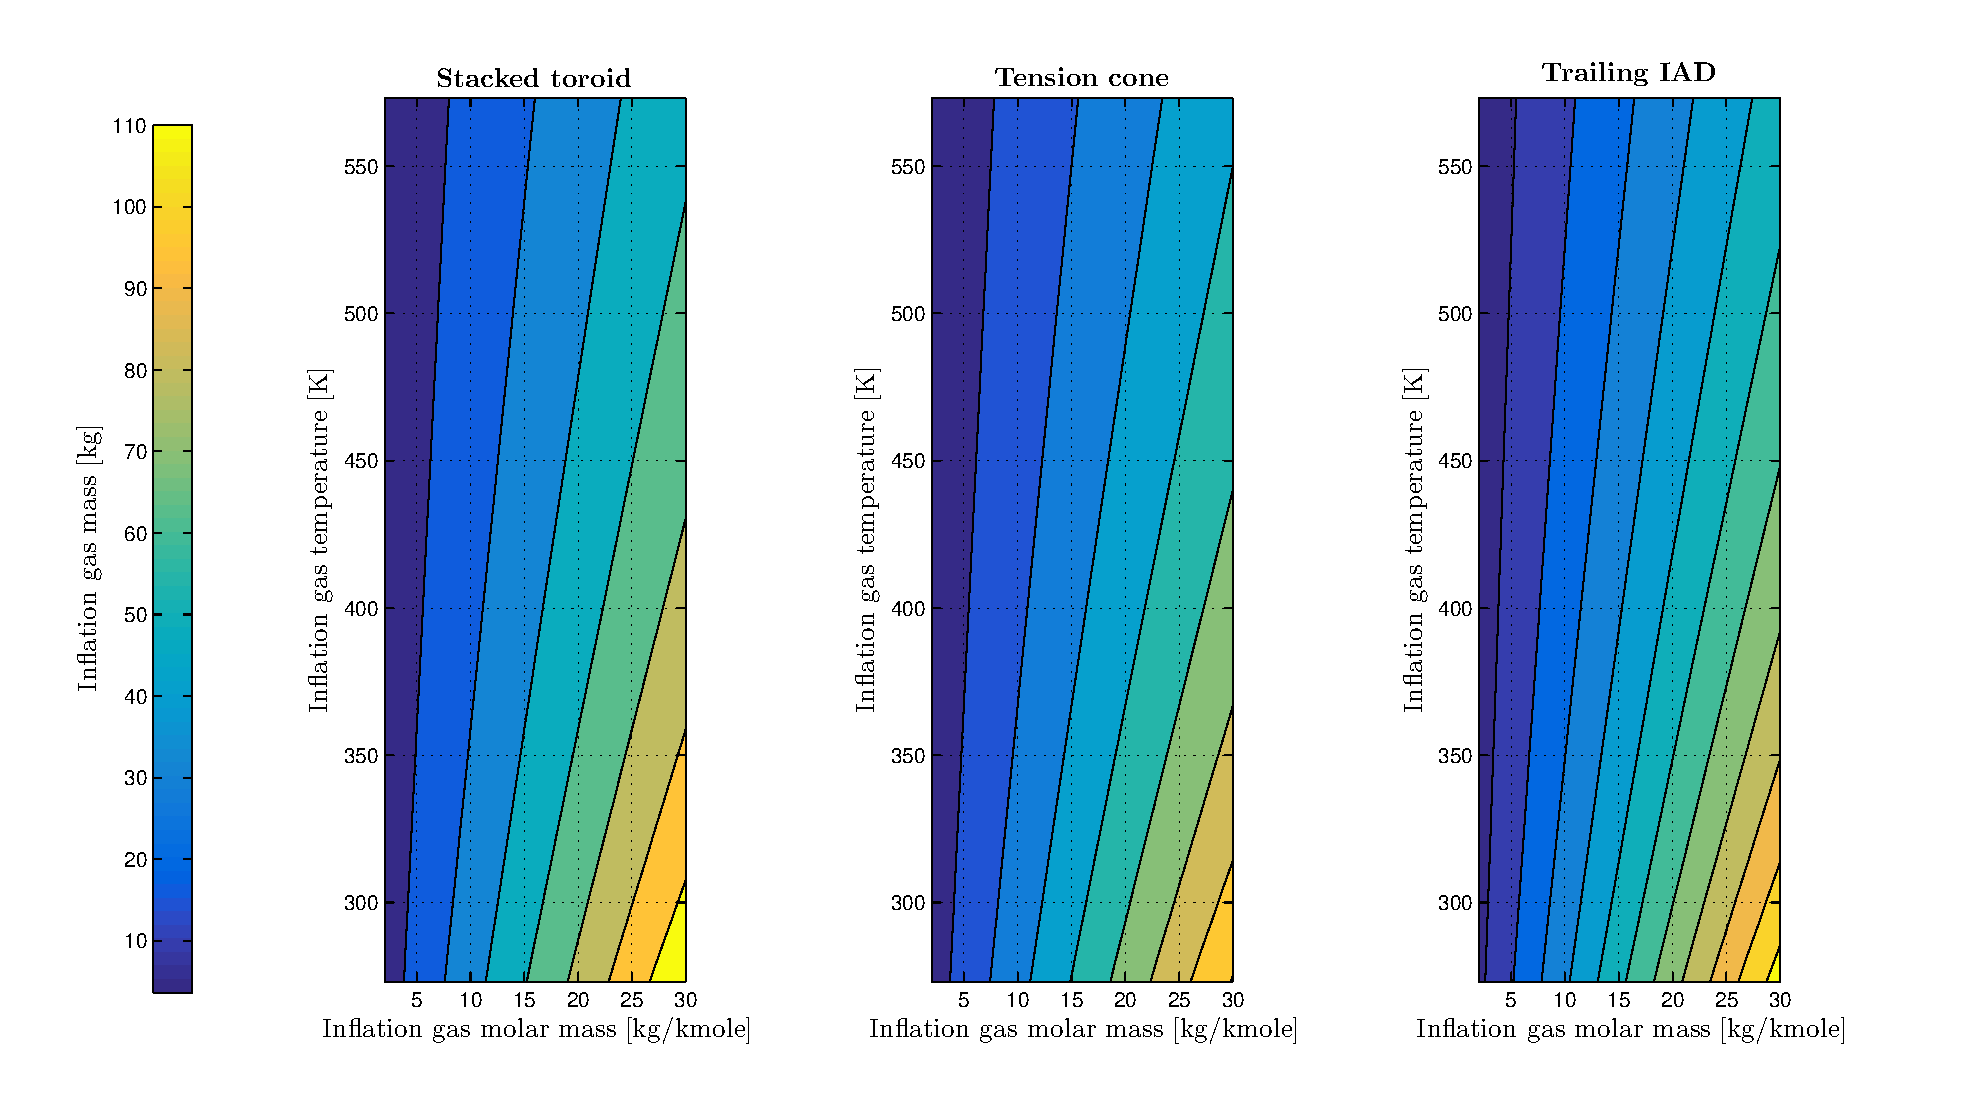
\includegraphics[width = 1.1\textwidth]{Figure/gas_temp_mass.eps}
\caption{Inflation gas mass as a function of gas temperature and molar mass of the stacked toroid, tension cone and trailing ballute configurations}
\label{fig:inflmass}
\end{figure}

Fig.\ref{fig:inflmass} confirms that a denser gas, characterized by a higher molar mass, yields a larger inflation gas mass. An overview of gas generator types and their output is given on page 7 by Brown \cite{Brown2003}. A typical molar mass is that of nitrogen, 22 [$\frac{kg}{mole}$], used in the IRVE satellites \cite{Dillman2012}. It should be noted that inflation system mass is typically estimated as a percentage of inflation gas mass. Total inflation system mass, thus consisting of inflation system and inflation gas mass, will therefore not be as low as suggested by Fig.\ref{fig:inflmass} for low molar mass inflation gases, but it will typically be higher by requiring a heavier inflation system \cite{Brown2003}. Inflation gas mass decreases for an increasing inflation gas temperature, again conforming to expectations. Via the ideal gas law the mass occupied by a certain number of moles of inflation gas will increase for a decreasing temperature through an increased gas density \cite{AndersonJr.2007}.

\subsubsection{Number of toroids for the stacked toroid configuration}
The stacked toroid features a number of toroids that are inflated. To investigate the effect of the number of toroids on total structural decelerator mass, the two are plotted against one another in Fig.\ref{fig:toro}. 

\begin{figure}[H]
\centering
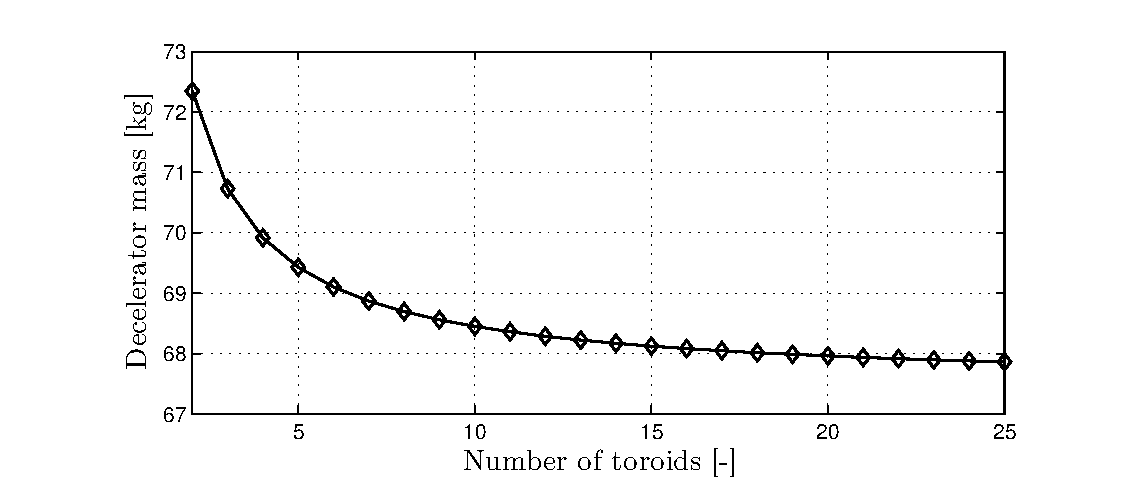
\includegraphics[width = 1.0\textwidth]{Figure/mass_toroids.eps}
\caption{Decelerator structural mass as a function of the number of toroids for the stacked toroid configuration}
\label{fig:toro}
\end{figure}

From Fig.\ref{fig:toro}, it may be observed that stacked toroid structural mass decreases for an increasing number of toroids. The decrease is, however, so slight as to be insignificant. A mass decrease of approximately 4 $\%$ is effected by an increase from one to five toroids; a decrease of approximately 5 $\%$ for an increase from one to ten toroids. As the number of toroids is increased beyond ten, mass is more or less constant. Total structural decelerator mass is therefore deemed indifferent to the number of toroids. Care should still be taken to attach too much value to the results yielded by the model, given its limited fidelity.

\subsubsection{Inflatable decelerator diameter}
Figures \ref{fig:mass_dia} and \ref{fig:bc_dia} illustrate the effect of a change in inflatable decelerator diameter on its structural mass. Fig.\ref{fig:mass_dia} illustrates that an increase in deployed diameter, given a certain peak dynamic pressure and drag coefficient, effects an exponential increase in decelerator mass. This increase is significant, adding as much as 33 $\%$ of structural mass for a tension cone for an increase in diameter from 13 to 14 [m], for a peak dynamic pressure of 3000 [Pa] and a drag coefficient of 1.5 [-]; the other concepts exhibit similar increases. A better estimate of the mass-effectiveness for an increasing diameter is given by Fig.\ref{fig:bc_dia}, which displays the ballistic coefficient of the decelerator, taking into account only its structural mass. This figure shows that the ballistic coefficient increases with increasing diameter for stacked toroid, tension cone and trailing ballute, denoting that decelerator structural mass increases more than its decelerating capability (the product of \gls{sym:CD} and \gls{sym:A_iad}) and thus that it becomes less mass-effective for an increasing deployed diameter. For the isotensoid, [ALEXANDER MINIMUM GAGE ISOTENSOID UITLEG]

\begin{figure}[H]
\centering
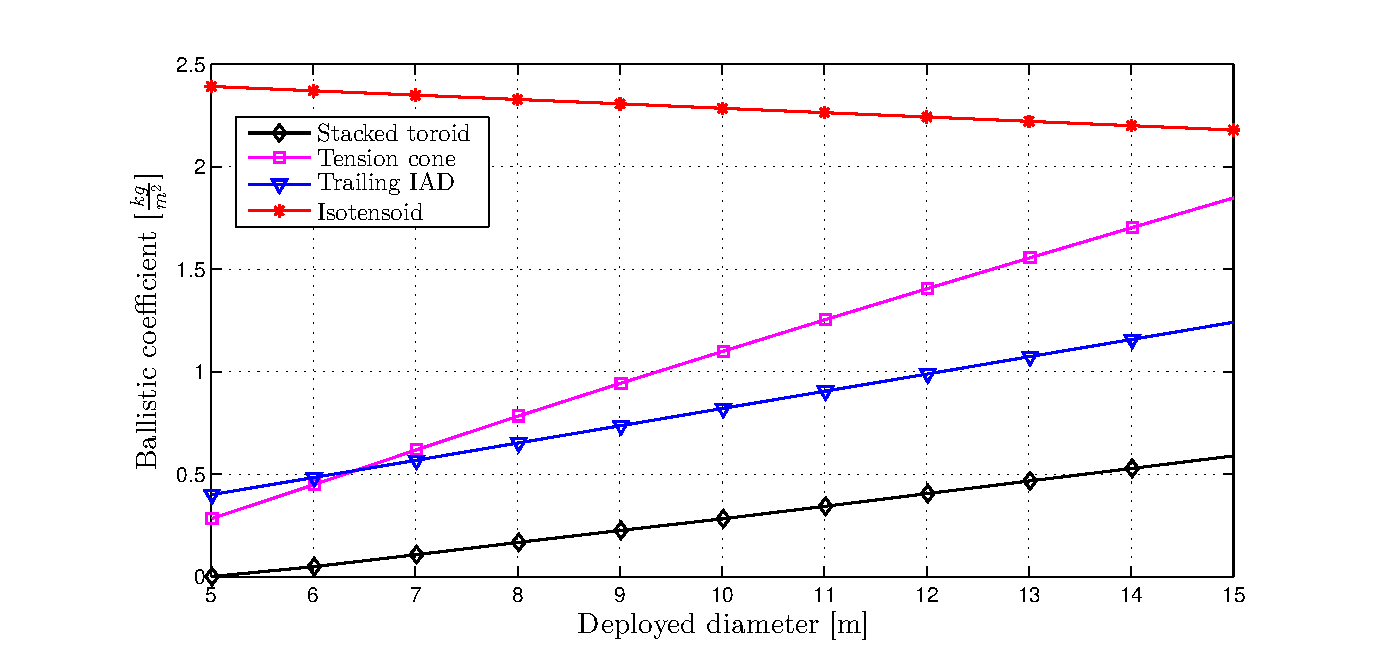
\includegraphics[width = 1.0\textwidth]{Figure/bc_dia.eps}
\caption{Decelerator structural ballistic coefficient as a function of deployed diameter of inflatable concepts}
\label{fig:bc_dia}
\end{figure}

\subsubsection{a}

\begin{figure}[H]
\centering
\includegraphics[width = 1.0\textwidth]{Figure/mass_theta_cd.eps}
\caption{Decelerator structural ballistic coefficient as a function of deployed diameter of inflatable concepts}
\label{fig:mass_theta_cd}
\end{figure}
\subsection{Conclusion}\label{sec:strucconc}


\section{Thermal mass estimation}
\label{ch:thermtool}
Decelerating an entry vehicle requires a thermal protection system. This system will contribute to a large extend to the mass of the entire vehicle. Therefore, a thermal protection system (\gls{tps}) has a critical impact on the mission an should be selected properly. This section will analyse the \gls{tps} of the five trade-off concepts with the use of a thermal protection tool. First the tool will be described in more detail. Afterwards it is described how the tool is verified and validated. In the third section, this tool will be used to analyse different lay-ups for the concepts under anlysis. As a result,the \gls{tps} masses for differnt concepts can be determined. Lastly, concluions and recomendations.

\subsection{Method of thermal analysis}
A mass estimations of the \gls{tps} requires analysis due to heat transfer in the heat shield. Enable to analyse different lay-ups in a short amount of time, it will be usefull to make use of a \gls{tps} tool. The working principles of this tool are describes in detail in this section.

\subsubsection{Assumptions}


\subsubsection{Leading equations}
Suthes
\subsubsection{Input}
Lucas
\subsubsection{Output}
Suthes


\subsection{Verification \& Validation}

\subsubsection{Verification}
Suthes
\subsubsection{Validation}



\subsection{Results per concept}



\subsection{Conclusion \& recomendations}

\section{Risk assessment}
\label{ch:riskestimation}
Development risk will be used as one of the trade-off criteria. 

\begin{table}[h]
	\centering
	\caption{Risk map elements}
	\label{tab:riskmapelements}
	\begin{tabular}{|c|c|}
		\hline 
		\textbf{Number} & \textbf{Element} \\ \hline \hline
		1 & \acrlong{tps} \\
		2 & Deployment mechanism \\
		3 & Aerodynamic characteristics \\
		4 & \\
		\hline
	\end{tabular}
\end{table}

\begin{table}[h]
	\caption[\acrlong{nasa} \acrfullpl{trl}]{\gls{nasa} \glspl{trl} \cite{NASA2007}}
	\begin{tabular}{|p{0.2\textwidth}|p{0.75\textwidth}|}
		\hline
		\textbf{\acrfull{trl}} & \textbf{Description} \\ \hline \hline
		\gls{trl} 9& Actual system "flight proven" through successful mission operations\\
		\gls{trl} 8& Actual system completed and "flight qualified" through test and demonstration (ground or space)\\
		\gls{trl} 7& System prototype demonstration in a space environment\\
		\gls{trl} 6& System/subsystem model or prototype demonstration in a relevant environment (ground or space)\\
		\gls{trl} 5& Component and/or breadboard validation in relevant environment\\
		\gls{trl} 4& Component and/or breadboard validation in laboratory environment\\
		\gls{trl} 3& Analytical \& experimental critical function and/or characteristic proof-of-concept\\
		\gls{trl} 2& Technology concept and/or application formulated\\
		\gls{trl} 1& Basic principles observed \& reported \\
		\hline
	\end{tabular}
\end{table}

\begin{table}[H]
	\centering
	\caption{Risk map}
	\label{tab:riskmap}
	\begin{tabular}{|c|c|c|c|c|} % MAKE SURE THAT THE TOTAL WIDTH IS 0.95\textwidth!! (that way its exactly the textwidth.... haha) 
		\hline
		\textbf{\gls{trl} 1} & \cellcolor{green!70} & \cellcolor{yellow!75} & \cellcolor{red!60} & \cellcolor{red!60} \\ \hline
		\textbf{\gls{trl} 2} & \cellcolor{green!70} & \cellcolor{yellow!75} & \cellcolor{red!60} & \cellcolor{red!60} \\ \hline
		\textbf{\gls{trl} 3} & \cellcolor{green!70} & \cellcolor{yellow!75} & \cellcolor{red!60} & \cellcolor{red!60} \\ \hline
		\textbf{\gls{trl} 4} & \cellcolor{green!70} & \cellcolor{yellow!75} & \cellcolor{yellow!75} & \cellcolor{yellow!75} \\ \hline
		\textbf{\gls{trl} 5} & \cellcolor{green!70} & \cellcolor{green!70} & \cellcolor{yellow!75} & \cellcolor{yellow!75} \\ \hline
		\textbf{\gls{trl} 6} & \cellcolor{green!70} & \cellcolor{green!70} & \cellcolor{green!70} & \cellcolor{green!70} \\ \hline
		\textbf{\gls{trl} 7} & \cellcolor{green!70} & \cellcolor{green!70} & \cellcolor{green!70} & \cellcolor{green!70} \\ \hline
		\textbf{\gls{trl} 8} & \cellcolor{green!70} & \cellcolor{green!70} & \cellcolor{green!70} & \cellcolor{green!70} \\ \hline
		\textbf{\gls{trl} 9} & \cellcolor{green!70} & \cellcolor{green!70} & \cellcolor{green!70} & \cellcolor{green!70} \\ \hline
		 & \textbf{Negligible} & \textbf{Marginal} & \textbf{Critical} & \textbf{Catastrophical} \\ \hline
	\end{tabular}
\end{table}

\subsection{Concept development risk}

The classification of selected concepts in terms of technology readiness serves to aid in the selection of a final concept that features minimal development risk. Since the selection is a relative process, technology readiness levels used hereafter are primarily intended for use with respect to each other rather than by themselves. For one, none of past inflatable missions have been flown with the dimensions considered nor were they suitable for human spaceflight.

Rigid concepts have long been the standard for manned (re-)entry missions and have been applied numerous times, as investigated in the Baseline Report \cite[p.2-3]{Balasooriyan2015a}. An overview of rigid (re-)entry vehicles is given by Laub et al. \cite{Laub2004} and Steinfeldt \cite{Steinfeldt2009} and were already used in the rigid concept mass estimation of section \ref{sec:rigid}. In addition, recent application in Mars missions, for example the Mars Science Laboratory \cite{Schoenenberger2009}, make the rigid concept a low development risk option. In terms of \gls{trl}, the rigid concept is therefore classified as \gls{trl} 9.

Inflatable concepts are still at a low technology readiness level. Whereas research efforts have been instigated as early as in the 1960s, a lull in research efforts up to recent years make the field of inflatable aerodynamic decelerators relatively underveloped \cite{Smith2010}. Hypersonic aerodynamic decelerator technology in particular has seen little application. Past and ongoing research by \gls{nasa} in hypersonic aerodynamic decelerators has focused on the stacked toroid configuration. A research programme consisting of a series of experiments, called \acrfull{irve}, was initiated in 2003 and the IRVE-II flight has brought the development risk of the stacked toroid configuration (as applied in the IRVE vehicles) to \gls{trl} 7 \cite{Player2005}.

Isotensoid, tension cone and ballute configurations have been tested primarily for supersonic entry (at Mach numbers lower than 5). Research efforts concentrated thereon have taken place primarily in the 1960s \cite{Smith2010}. A lack of research programmes on these configurations in recent years and the series of laboratory tests conducted in the 1960s have led to designating these concepts with a \gls{trl} of 4.

Moreover, the discussion on trailing ballute controllability in Chapter \ref{ch:astrocontrol} limits the range of control systems to morphing. This control method, as argued in that chapter, is highly undeveloped for space applications and remains untested. As such, it is a concept that remains formulated with a corresponding \gls{trl} of 2.

An overview of development risk for the five concepts is given in Table \ref{tab:concrisk}.

\begin{table}[h]
\centering
\caption{Concept development risk comparison}
\begin{tabular}{|l|l|l|l|l|l|}
\hline
\textbf{Concept {[}-{]}} & Stacked toroid & Tension cone & Trailing ballute & Isotensoid & Rigid \\ \hline
\textbf{TRL {[}-{]}}     & 7              & 4            & 2                & 4          & 9     \\ \hline
\end{tabular}
\label{tab:concrisk}
\end{table}


\section{Concept performance in trade-off criteria}\label{ch:tfsum}

 A conceptual analysis, described in previous chapters, has been performed to establish concept performance in terms of these criteria. Dialogue with the customer during the \acrfull{mtr} yields a decision for a final concept for preliminary analysis and design. This chapter treats the concept performance for all five selected concepts in terms of the trade-off criteria formulated in Chapter \ref{ch:tradeoff}, namely: decelerator mass, development risk, deceleration time and stability. Control system, \acrfull{tps} and structural masses are distinguished within decelerator mass. Subsequent sections detail concept performance in terms of each of the trade-off criteria.

\subsection{Decelerator mass}
Concepts have been evaluated for the three primary components that make up and distinguish concepts: structure, \acrfull{tps} and control system. The structural mass has been estimated using parametric models in Chapter \ref{ch:strucmass}; the \gls{tps} mass via a basic thermal layer analysis in Chapter \ref{ch:thermtool}; the control system mass via the required moments to be generated in Chapter \ref{ch:astrocontrol}.  These masses are given in Table \ref{tab:cmass}. It should be noted that the structural mass excludes connection mass, not taken into account in the mass estimation and deemed equal for all concepts. Hence the summed mass consists of only 85 $\%$ of the decelerator mass. 

While structural mass has been estimated directly in [kg], the thermal and control system mass, following from Chapters \ref{ch:thermotool} and \ref{ch:controlmass}, have been estimated on the basis of heat load and moment coefficients. Since the comparison requires only relative masses, all  masses have been expressed as a percentage of stacked toroid mass. Total mass is calculated as the weighted average of the three weight components. Each of the components, structural mass, thermal mass and control system mass, has been given an importance factor, of respectively 20 $\%$,  50 $\%$ and  15 $\%$ corresponding to the weight fraction assigned in the budget breakdown in the Baseline Report \cite[p.28]{Balasooriyan2015a}. These weights have been used since masses are used for relative comparison and the subsystems contribute in a different magnitude to the total decelerator mass. These importance factors are the best available estimates for their corresponding weight fractions, given the limited analysis possibilities.

\begin{table}[h]

\caption{Concept mass comparison (expressed as percentage of stacked toroid mass)}\label{tab:cmass}
\hspace{-10mm}
\begin{tabular}{|p{0.2\textwidth}|p{0.2\textwidth}|p{0.2\textwidth}|p{0.2\textwidth}||p{0.079\textwidth}|}

\hline
                          & \textbf{Structural mass (20 \%)} & \textbf{Thermal mass (50 \%)} & \textbf{Control system mass (15 \%)} & \textbf{Total mass} \\ \hline
\textbf{Stacked toroid}   &  100                                 & 100                          & 100                                      &\cellcolor{green!70}  100                           \\ \hline
\textbf{Tension cone}     &  168                               & 100                               &  100                                     &\cellcolor{green!70} 116                                 \\ \hline
\textbf{Trailing ballute} &  221                                 & 84                               & 86                                      &\cellcolor{green!70} 117 \\ \hline
\textbf{Isotensoid}       &  516                                 & 76                               & 99                                      &\cellcolor{yellow!75} 184 \\ \hline \hline
\textbf{Rigid}            &  \multicolumn{4}{|p{0.762\textwidth}|}{\cellcolor{red!60} ~~~~~~~~~~~~~~~~~~~~~~~~~~~~~Far in excess of 1000 [kg] limit}    \\ \hline
\end{tabular}
\end{table}

From the last column in Table \ref{tab:cmass} it follows that the lowest estimated decelerator mass is achieved using the stacked toroid configuration. Evidently the highest mass is achieved by the rigid concept, with an estimated combined structural and thermal mass of 2945 [kg] (see section \ref{sec:rigid}) well in excess of the 1000 [kg] limit imposed. The latter is therefore deemed unacceptable; the former is deemed excellent performance. The isotensoid performs notably worse (184 \% of stacked toroid mass), while stacked toroid, tension cone and trailing ballute perform similarly (at 100, 116 and 117 \% of stacked toroid mass).

As discussed previously, a lower decelerator mass (denoted by the total mass column in Table \ref{tab:cmass}) effectively means a larger payload mass given the objective of fully using launcher capability by a total entry vehicle mass of 10000 [kg]

\subsection{Development risk}
Development risk has been evaluated on the basis of concept technology readiness in Chapter \ref{ch:riskestimation}. It was concluded that frequent historic investigation, testing and application of rigid concepts for (re-)entry make this concept the most developed and full-scale and relevant environment testing yield \acrfull{trl} 9. Inflatable concepts are a relatively novel solution and investigation thereof has been limited: isotensoid, trailing ballute and tension cone concepts have been tested up to an estimated \gls{trl} of 4. The stacked toroid concept has undergone a more extensive research program (\acrfull{irve}) and is hence at a \gls{trl} of 7 while ongoing research by \gls{nasa} continues to further the technology readiness \cite{Dillman2014}. It should be noted that the trailing ballute is only capable of featuring morphing as a viable control option, as investigated in Chapter \ref{ch:astrocontrol}, an underdeveloped area of technology for the application at hand. To reflect the difficulty of control with a trailing ballute, its \gls{trl} is lowered to 2 since morphing has only been formulated, but not tested, for this concept.

The \glspl{trl} of the five selected concepts are stated in Table \ref{tab:gls_rev}.

\begin{table}[h]
\caption{Review of concept development risk}
\begin{tabular}{|l|l|l|l|l|l|}
\hline
\textbf{Concept {[}-{]}} & Stacked toroid & Tension cone & Trailing ballute & Isotensoid & Rigid \\ \hline
\textbf{TRL {[}-{]}}     &\cellcolor{green!70} 7  &\cellcolor{yellow!75}  4   &\cellcolor{red!60} 2 & \cellcolor{yellow!75}      4          &\cellcolor{green!70} 9     \\ \hline
\end{tabular}
\label{tab:gls_rev}
\end{table}

\subsection{Deceleration time}
The deceleration time is evaluated on the basis of vehicle lift gradient, taken as the average over a range of considered angles of attack. A higher ligt gradient is thereby deemed positive in achieving deceleration within a shorter time. This evaluation, discussed in Chapter \ref{ch:aero_analysis}, has yielded the results given in Table \ref{tab:decel_time}.

\begin{table}[h]
\caption{Review of concept lift gradient}
\hspace{-20mm}
\begin{tabular}{|c|c|c|c|c|c|}
\hline
\textbf{}                          & \textbf{Stacked toroid} & \textbf{Tension cone} & \textbf{Trailing ballute} & \textbf{Isotensoid} & \textbf{Rigid} \\ \hline
\textbf{Average lift gradient {[}1/rad{]}} &\cellcolor{green!70} 7  &\cellcolor{yellow!75}  4   &\cellcolor{red!60} 2 & \cellcolor{yellow!75}      4          &\cellcolor{green!70} 9                 \\ \hline
\end{tabular}
\end{table}

From Table \ref{tab:decel_time} it may be observed that the highest lift gradient is attained for the ... configuration. [ADD AERO EXPLANATION]

\subsection{Stability}
Stability of concepts is measured by the static stability, as explained in Chapter \ref{ch:aero_analysis}. A more stable concept is reflected by a more negative static stability coefficient. This derivative is given in Table \ref{tab:stab}.

\begin{table}[h]
\caption{Review of concept lift gradient}
\hspace{-20mm}
\begin{tabular}{|c|c|c|c|c|c|}
\hline
\textbf{}                          & \textbf{Stacked toroid} & \textbf{Tension cone} & \textbf{Trailing ballute} & \textbf{Isotensoid} & \textbf{Rigid} \\ \hline
\textbf{Static stability coefficient {[}1/rad{]}} &\cellcolor{green!70} 7  &\cellcolor{yellow!75}  4   &\cellcolor{red!60} 2 & \cellcolor{yellow!75}      4          &\cellcolor{green!70} 9                 \\ \hline
\end{tabular}
\end{table}

[ADD AERO EXPLANATION]


\section{Conclusion}\label{cha:conclusion}

\subsection{Requirements}
In this section the top-level requiremets are stated. They can be found in table \ref{tab:requirements}.

\begin{table}[H]
	\caption {Requirement}
    \begin{tabular}{|l|l|}
    \hline
    Code          & Description                                                                                                      \\ \hline
    CIA-Sys-A01-1 & The re-entry vehicle shall be able to cope with an entry velocity of seven kilometers per second.                \\ \hline
    CIA-Sys-A01-2 & The inflated aeroshall shall have a maximum diameter of 12 meters.                                               \\ \hline
    CIA-Sys-A01-3 & The diameter of the launcher fairing shall be 5 meters.                                                          \\ \hline
    CIA-Sys-A01-4 & The maximum entry mass of the re-entry vehicle shall be 10,00 kilograms.                                         \\ \hline
    CIA-Sys-A01-5 & The hypersonic deceleration system mass shall not be havier than ten percent of the total re-entry vehicle mass. \\ \hline
    CIA-Sys-A01-6 & The control system shall have a maximum failure probability of 5.0e-4.                                           \\ \hline
    CIA-Sys-A01-7 & The maximum allowable loads on the re-entry vehicle shall be 3 earth g's in each axis                            \\ \hline
    CIA-Sys-A01-8 & The re-entry vehicle shall have a maximal aerobraking duration of ten days.                                      \\ \hline
    \end{tabular}
    \label{tab:requirements}
\end{table}



\subsection{System description}


% Bibliography
\newpage
\bibliography{./Bibliography/Bibliography}
\bibliographystyle{ieeetr}
% Appendix
\newpage
\appendix
\section{Requirements overview} \label{app:req}

\begin{table}[H]
	\caption*{Overview of high level mission requirements} \label{tab:toplevelreq}
	\begin{tabular}{|p{0.20\textwidth}|p{0.7\textwidth}|}
    \hline
    ID          & Description                                                                                                      \\ \hline \hline
    CIA-Func & The re-entry vehicle shall decelerate from a velocity of 7 $[\frac{km}{s}]$ to a velocity of \gls{tbd} $[\frac{km}{s}]$  \\ \hline
    CIA-Op & The re-entry vehicle shall operate within mission constraints                                               \\ \hline
& \\ \hline
    CIA-Func-A01 & The re-entry vehicle shall decelerate from a velocity of 7 $[\frac{km}{s}]$ to a velocity of \gls{tbd} $[\frac{km}{s}]$     \\ \hline
    CIA-Func-A02 & The re-entry vehicle shall not exert an acceleration greater than 29.4 $[\frac{m}{s^2}]$ on any crew member for the duration of the mission			\\ \hline
    CIA-Func-A03 & The re-entry vehicle shall not be heated excessively  \\ \hline
    CIA-Func-A04 & The re-entry vehicle shall be in a controlled state for the duration of the mission                            \\ \hline
& \\ \hline
    CIA-Op-A01 & The re-entry vehicle shall meet all geometric constraints imposed by the mission                           \\ \hline
    CIA-Op-A02 & The re-entry vehicle shall meet all mass constraints imposed by the mission                                      \\ \hline
	CIA-Op-A03 & The re-entry vehicle shall meet all payload constraints imposed by the mission \\ \hline
	CIA-Op-A04 & The re-entry vehicle shall attain its final velocity at an altitude of \gls{tbd} [m] \\ \hline
	CIA-Op-A05 & The re-entry vehicle shall attain its final velocity within 10 days of mission start \\ \hline
& \\ \hline
	CIA-Op-A01-01 & The reentry vehicle shall have an undeployed diameter smaller than 5 [m]                         				            \\ \hline
	CIA-Op-A01-02 & The reentry vehicle shall have a deployed diameter smaller than 12 [m]                         				            \\ \hline
	CIA-Op-A01-03 & The reentry vehicle shall have a volume capable of accommodating 6 crew members                        				            \\ \hline
	CIA-Op-A02-01 & The reentry vehicle shall have a mass of 10000 [kg] at the start of the re-entry                       				            \\ \hline
	CIA-Op-A02-02 & The hypersonic decelerator shall have a mass fraction of no greater than 10\% of the vehicle mass  \\ \hline
	CIA-Op-A02-03 & The crew module shall have a mass fraction of no greater than 90\% of the vehicle mass \\ \hline
	CIA-Op-A03-01 & The reentry vehicle shall carry sufficient provisions for the crew for the duration of the mission \\ \hline
	CIA-Op-A03-02 & The reentry vehicle shall be able to carry the mission payload								\\ \hline	
    \end{tabular}
\end{table}


\begin{table}[h]
	\caption*{Overview of aerodynamic requirements}
	\label{tab:aeroreqs}
	\begin{tabular}{|p{0.2\textwidth}|p{0.7\textwidth}|}
		\hline
		ID & Description \\
		\hline \hline
		CIA-Func-B01-Aero-01 & The system shall have a \gls{sym:CD}\gls{sym:A} of at least TBD $m^{2}$ \\ \hline
		CIA-Func-B02-Aero-02 & The system shall have a \gls{sym:CD}\gls{sym:A} of at most TBD $m^{2}$ \\ \hline
		CIA-Func-B03-Aero-03 & The system shall produce a maximum heat flux of no more than TBD [$\frac{W}{cm^{2}}$] \\ \hline
	\end{tabular}
\end{table}

\begin{table}[H]
	\caption*{Overview of structural requirements}
	\begin{tabular}{|p{0.20\textwidth}|p{0.70\textwidth}|}
    \hline
    ID          & Description                                                                                                      \\ \hline \hline
    CIA-Func-B01-Struc-01 & The structure shall support deployment \\ \hline
    CIA-Func-B02-Struc-02 & The structure shall sustain the maximum mechanical loads without failure                           \\ \hline
    CIA-Func-B04-Struc-03 & The structure shall connect payload and deceleration mechanism \\ \hline
    CIA-Func-B04-Struc-04 & The structure shall not deform excessively \\ \hline
    CIA-Op-B01-01-Struc-05 & The structure shall have a maximum diameter not exceeding 5 [m] in stowed configuration                              \\ \hline
    CIA-Op-B01-02-Struc-06 & The structure shall have a maximum diameter not exceeding 12 [m] in deployed configuration     \\ \hline
    CIA-Op-B02-Struc-07 & The structure shall have a mass not exceeding 350 [kg]\\ \hline
    \end{tabular}
    \label{tab:strucfuncrequirements}
\end{table}

\begin{table}[H]
	\caption*{Overview of thermal requirements}
	\begin{tabular}{|p{0.2\textwidth}|p{0.70\textwidth}|}
    \hline
    ID          & Description                                                                                                      \\ \hline \hline
   CIA-Func-B03-TPS-01 & The TPS shall be able to withstand the maximum heat flux of \gls{tbd} $ \left[\frac{W}{cm^2}\right] $               
\\ \hline
    CIA-Func-B03-TPS-02 &  The TPS shall be able to withstand the maximum heat load of \gls{tbd} $ \left[\frac{J}{cm^2}\right] $               
\\ \hline
    CIA-Func-B03-TCS-01 & The TCS shall keep the subsystems within their operative temperature range                                            
\\ \hline
    CIA-Func-B03-TCS-02-crewmodule & The TCS shall keep the crew module within a temperature range of \gls{tbd} and \gls{tbd} $ \left[^{\circ}C\right] $                                        
\\ \hline
    CIA-Func-B03-TCS-03-structure & The TCS shall keep the structure module within a temperature range of \gls{tbd} and \gls{tbd} $ \left[^{\circ}C\right] $                                        
\\ \hline
	CIA-Op-B02-Therm-01 	&	The thermal system shall have a mass not exceeding 500 [kg]  							\\ \hline
    \end{tabular}
    \label{tab:thermalreq}
\end{table}

\begin{table}[H]
	\caption*{Overview of Control requirements}
	\begin{tabular}{|p{0.2\textwidth}|p{0.70\textwidth}|}
		\hline
		ID         					&	Description																							\\ \hline \hline
		CIA-Func-B04-Contr-01		&	The control system shall have a reliability of $5 \cdot 10^{-4}$            									\\ \hline
		CIA-Func-B04-Contr-02 		&	The control system shall keep the spacecraft within a distance to the trajectory of \gls{tbd} [m]	\\ \hline	
		CIA-Func-B04-Contr-02-01 	&	The control system shall provide (augmented) dynamic stability       								\\ \hline
		CIA-Func-B04-Contr-02-02 	&	The control system shall provide attitude control over three axes         							\\ \hline	
		CIA-Op-Contr-B04-03	&	The control system shall have a mass not exceeding 150 [kg]  							\\ \hline
	\end{tabular}
	\label{tab:controlreq}
\end{table}

\section{Organisational Function Description} \label{app:obs}
The functions, as described in section \ref{sec:org}, entail the following responsibilities.

\subsection{Organisational functions}
\subsubsection{Chairman}\label{subsec:Chairman}
The size of the DSE project group, with 9 people, is too large to be self-organizing: if no organizational structure is apparent, people will not have a clear view of the required work, leading to inefficient time-management. The role of the chairman is to prepare team meetings and guide them such that the meeting itself is performed in an efficient manner, but also the goal of the meeting is achieved: at the end of the meeting, all team members should have a clear overview of the current status of the project, as well as their present responsibilities. It is the task of the chairman to guide meetings such that this information is conveyed between the team members including the members responsible for planning, documentation, and the system engineer. Concretely, this also encompasses making the agenda.

\subsubsection{Secretary}\label{subsec:Secretary}
	The secretary shall minute during both project and customer meetings and keep track of design decisions and how they are made. This is done to assure that changes in the design process can be reviewed and remember why changes are made the way they are made. Furthermore, the secretary shall be responsible for all internal and external communication.

\subsubsection{Documentation manager}\label{subsec:D_and_A}
One of the tasks of the documentation manager is to maintain a structure in the file system used on the computer (i.e. keeping Dropbox and Github organized). The documentation manager is also the person to set up the initial files (like the LaTeX templates) and folder structures. The documentation manager should provide basic rules for the layout of the documents, communication with the editor is needed when the layout does not conform these rules. It is needed that this structure is maintained throughout the project and group members should make an effort to keep it this way, if not it is the documentation manager that will point out these problems towards the group and come with possible solutions. 

\subsubsection{Planner}\label{subsec:Planner}
The planner provides an overview for all the work packages as progressing through to time in the form of a Gantt chart. It is the function of the planner to frequently update and further detail this chart throughout the progress of the project. Furthermore more the planner is required to communicate all deadlines to the group members. Interactions between different tasks are provided and planning is made accordingly to allow all tasks to be finished before the set deadlines or milestones. Progression is recorded throughout the process to ascertain that all deadlines are met. 



\subsubsection{Systems engineer}\label{subsec:SE}
The systems engineer is responsible for the overall technical progress of the project. He keeps track of the project requirements and manages the interfaces between different design disciplines. His responsibilities can be summarized as follows:

\begin{itemize}
\item Track project requirements and overall technical progress
\item Manage design interfaces between design disciplines
\item Resolve design conflicts due to conflicting requirements 
\end{itemize}


\subsubsection{Risk Engineer}\label{subsec:RiskEng}
To mitigate cost or time overruns or even worse, eventual product failure, risk management plays a central role within project management. In order to properly address the risks involved in developing an inflatable aeroshell one person is ultimately responsible for possible hazard management: The risk engineer. The task of this risk engineer is to manage the various risks encountered during the design process. This will be done by using technical budgeting to manage the performance risks during the various design phases. Performance margins can be defined for each system and subsystem that influence the performances of other systems. In addition to this risk mapping will be used. By identifying critical components of each proposed concept and allocating the available resources accordingly the project risks can be minimized. Risk management is a continuous process.

\subsubsection{Quality assurance}\label{subsec:QA}
\paragraph{Editor}
Primary function is assuring consistent and high quality of all written communication, by means of proof-reading and correcting of pieces submitted by all group members. In addition, the lay-out and structure of reports and presentations is scrutinized and egalized. Strong interaction takes place with all group members with direct contributions to the written work, while open communication with documentation manager is maintained to resolve issues with the formatting of reports. In case of repeated errors by group members, the editor makes an effort to enter conversation with the repeaters in order to identify the origin of the problem and if need be to take pre-emptive action against future occurrences.
\paragraph{Verification}
Verification occurs at multiple stages of the design. For one, concepts should be verified to check whether the developed product meets the requirements. The team member in charge of verification

\paragraph{Validation}
IEEE defines validation as ''The assurance that a product, service, or system meets the needs of the customer and other identified stakeholders. It often involves acceptance and suitability with external customers.''(ref. ''IEEE V\&V.pdf'') The person in charge of validation is thus responsible for the compliance of the product with the requirements imposed by the costumers and stakeholders. Another task is to assure that the subsystem requirements contribute to accomplishing the system requirements and in the end to the top level requirements.


%\subsection{Engineering breakdown}\label{subsec:engineer}
%The engineering work of the controllable inflatable aeroshell is divided into different departments. These departments are the driving fields in the design of an inflatable aeroshell and will cover all aspects of the design. As for the management positions, engineering departments are not isolated in the sense that the aim is to involve team members in multiple design aspects.

\subsection{Technical functions}
\subsubsection{Aerodynamics department}\label{subsec:aero}
The aerodynamics department will look at different shapes possible to do the entry in the Martian atmosphere. This department looks at the hypersonic aerodynamics and determines the amount of thermal energy the heat shield needs to absorb and the loads that the structure needs to endure. In addition, the creation of a aerodynamic model of the vehicle that will be used in the control system is produced by the aerodynamics department.

\subsubsection{Structures department}\label{subsec:struct}
The structures department is responsible for the design of the structure, carrying primarily the mechanical and thermal loads by aerodynamic forces and heating. This design entails appropriate material selection, design and sizing of load-carrying elements and integrating the design while maintaining feasibility in terms of manufacturability, costs and weight. For the purpose of determining structural performance, the structures department is responsible for the development of structural tools. Moreover, the structures department actively communicates with other departments to synthesize the system design.

\subsubsection{Control systems department}\label{subsec:control}
The control systems department will analyse the controllability and stability, both static and dynamic, of the vehicle. Further this department will design the subsystems that will provide the needed characteristics for the controllability and stability. The control department covers all additional subsystems to ensure a controllable and stable vehicle, i.e. an attitude determination system. It will also create the astrodynamic mission profile to be used during the re-entry, and will create a model of the Martian atmosphere to use during the determination of this profile.

\subsubsection{Thermal control department}\label{subsec:therm}
The thermodynamics department will look at the thermal aspect of the inflatable aeroshell. The aerodynamics department will provide a boundary condition for the heat propagation within the structure. This heat propagation will be dependent on material properties and structure shape as defined by the structures department. Furthermore, the space vehicle should have thermal control such that systems can operate and humans can survive.
\section{Organisational Function Description} \label{app:obs}
The functions, as described in section \ref{sec:org}, entail the following responsibilities.

\subsection{Organisational functions}
\subsubsection{Chairman}\label{subsec:Chairman}
The size of the DSE project group, with 9 people, is too large to be self-organizing: if no organizational structure is apparent, people will not have a clear view of the required work, leading to inefficient time-management. The role of the chairman is to prepare team meetings and guide them such that the meeting itself is performed in an efficient manner, but also the goal of the meeting is achieved: at the end of the meeting, all team members should have a clear overview of the current status of the project, as well as their present responsibilities. It is the task of the chairman to guide meetings such that this information is conveyed between the team members including the members responsible for planning, documentation, and the system engineer. Concretely, this also encompasses making the agenda.

\subsubsection{Secretary}\label{subsec:Secretary}
	The secretary shall minute during both project and customer meetings and keep track of design decisions and how they are made. This is done to assure that changes in the design process can be reviewed and remember why changes are made the way they are made. Furthermore, the secretary shall be responsible for all internal and external communication.

\subsubsection{Documentation manager}\label{subsec:D_and_A}
One of the tasks of the documentation manager is to maintain a structure in the file system used on the computer (i.e. keeping Dropbox and Github organized). The documentation manager is also the person to set up the initial files (like the LaTeX templates) and folder structures. The documentation manager should provide basic rules for the layout of the documents, communication with the editor is needed when the layout does not conform these rules. It is needed that this structure is maintained throughout the project and group members should make an effort to keep it this way, if not it is the documentation manager that will point out these problems towards the group and come with possible solutions. 

\subsubsection{Planner}\label{subsec:Planner}
The planner provides an overview for all the work packages as progressing through to time in the form of a Gantt chart. It is the function of the planner to frequently update and further detail this chart throughout the progress of the project. Furthermore more the planner is required to communicate all deadlines to the group members. Interactions between different tasks are provided and planning is made accordingly to allow all tasks to be finished before the set deadlines or milestones. Progression is recorded throughout the process to ascertain that all deadlines are met. 



\subsubsection{Systems engineer}\label{subsec:SE}
The systems engineer is responsible for the overall technical progress of the project. He keeps track of the project requirements and manages the interfaces between different design disciplines. His responsibilities can be summarized as follows:

\begin{itemize}
\item Track project requirements and overall technical progress
\item Manage design interfaces between design disciplines
\item Resolve design conflicts due to conflicting requirements 
\end{itemize}


\subsubsection{Risk Engineer}\label{subsec:RiskEng}
To mitigate cost or time overruns or even worse, eventual product failure, risk management plays a central role within project management. In order to properly address the risks involved in developing an inflatable aeroshell one person is ultimately responsible for possible hazard management: The risk engineer. The task of this risk engineer is to manage the various risks encountered during the design process. This will be done by using technical budgeting to manage the performance risks during the various design phases. Performance margins can be defined for each system and subsystem that influence the performances of other systems. In addition to this risk mapping will be used. By identifying critical components of each proposed concept and allocating the available resources accordingly the project risks can be minimized. Risk management is a continuous process.

\subsubsection{Quality assurance}\label{subsec:QA}
\paragraph{Editor}
Primary function is assuring consistent and high quality of all written communication, by means of proof-reading and correcting of pieces submitted by all group members. In addition, the lay-out and structure of reports and presentations is scrutinized and egalized. Strong interaction takes place with all group members with direct contributions to the written work, while open communication with documentation manager is maintained to resolve issues with the formatting of reports. In case of repeated errors by group members, the editor makes an effort to enter conversation with the repeaters in order to identify the origin of the problem and if need be to take pre-emptive action against future occurrences.
\paragraph{Verification}
Verification occurs at multiple stages of the design. For one, concepts should be verified to check whether the developed product meets the requirements. The team member in charge of verification

\paragraph{Validation}
IEEE defines validation as ''The assurance that a product, service, or system meets the needs of the customer and other identified stakeholders. It often involves acceptance and suitability with external customers.''(ref. ''IEEE V\&V.pdf'') The person in charge of validation is thus responsible for the compliance of the product with the requirements imposed by the costumers and stakeholders. Another task is to assure that the subsystem requirements contribute to accomplishing the system requirements and in the end to the top level requirements.


%\subsection{Engineering breakdown}\label{subsec:engineer}
%The engineering work of the controllable inflatable aeroshell is divided into different departments. These departments are the driving fields in the design of an inflatable aeroshell and will cover all aspects of the design. As for the management positions, engineering departments are not isolated in the sense that the aim is to involve team members in multiple design aspects.

\subsection{Technical functions}
\subsubsection{Aerodynamics department}\label{subsec:aero}
The aerodynamics department will look at different shapes possible to do the entry in the Martian atmosphere. This department looks at the hypersonic aerodynamics and determines the amount of thermal energy the heat shield needs to absorb and the loads that the structure needs to endure. In addition, the creation of a aerodynamic model of the vehicle that will be used in the control system is produced by the aerodynamics department.

\subsubsection{Structures department}\label{subsec:struct}
The structures department is responsible for the design of the structure, carrying primarily the mechanical and thermal loads by aerodynamic forces and heating. This design entails appropriate material selection, design and sizing of load-carrying elements and integrating the design while maintaining feasibility in terms of manufacturability, costs and weight. For the purpose of determining structural performance, the structures department is responsible for the development of structural tools. Moreover, the structures department actively communicates with other departments to synthesize the system design.

\subsubsection{Control systems department}\label{subsec:control}
The control systems department will analyse the controllability and stability, both static and dynamic, of the vehicle. Further this department will design the subsystems that will provide the needed characteristics for the controllability and stability. The control department covers all additional subsystems to ensure a controllable and stable vehicle, i.e. an attitude determination system. It will also create the astrodynamic mission profile to be used during the re-entry, and will create a model of the Martian atmosphere to use during the determination of this profile.

\subsubsection{Thermal control department}\label{subsec:therm}
The thermodynamics department will look at the thermal aspect of the inflatable aeroshell. The aerodynamics department will provide a boundary condition for the heat propagation within the structure. This heat propagation will be dependent on material properties and structure shape as defined by the structures department. Furthermore, the space vehicle should have thermal control such that systems can operate and humans can survive.
\section{Trade off matrix} \label{app:trade}
The table on the next page shows the trade-off matrix for the final concept selection. The criterion weights are to be filled in during the \acrfull{mtr} in which a final concept will be selected. The content of this trade-off table is based on the results of this mid-term report which is also summarised in Chapter \ref{ch:tfsum}.

\newgeometry{margin=1.5cm}
\thispagestyle{empty}
\begin{landscape}
	\begin{tabular}{|C{3.45cm}||p{1.0cm}|p{1.0cm}|p{1.0cm}|p{1.0cm}|p{4.2cm}|p{4.2cm}|p{4.2cm}|}
		\hline
			 &\multicolumn{4}{p{0.763cm}|}{\textbf{Decelerator mass}} & \textbf{Development risk}& \textbf{Deceleration time }&\textbf{Stability} \\ \hline
		\textbf{Criterion weight} & \multicolumn{4}{p{0.763cm}|}{} &  &  &  \\ \hline \hline
		\textbf{Decelerator mass component}  &Struc- ture 20 \%&\gls{tps} \newline  \newline 50 \% &Con- trol 15\% & Total&  &  &    \\ \hline \hline
		\textbf{\newline \newline Stacked toroid} 	 & 100\% & 100\%  & 100\%  &\cellcolor{green!70} 100\% &\cellcolor{green!70} \gls{trl} 7 \newline series of \glspl{irve} by \gls{nasa} involving ground and flight tests in relevant environments & \cellcolor{yellow!75}          &\cellcolor{green!70} Static stability\\[12ex] \hline
		\textbf{\newline \newline Tension cone} 	 & 168\% & 100\%  & 100\% &\cellcolor{yellow!75} 116\%  &\cellcolor{yellow!75} \gls{trl} 4 \newline laboratory tests conducted & \cellcolor{yellow!75}             &\cellcolor{green!70} Static stability \\[12ex] \hline
		\textbf{\newline \newline Trailing ballute} & 221\% & 84\%   & 86\% &\cellcolor{yellow!75} 117\% &\cellcolor{red!60} \gls{trl} 2 \newline laboratory tests conducted, underveloped morphing control option & \cellcolor{yellow!75}           &\cellcolor{green!70} Static stability \\[12ex] \hline
		\textbf{\newline \newline Isotensoid}  & 105\% & 76\%   & 99\% &\cellcolor{green!70} 88\% &\cellcolor{yellow!75} \gls{trl} 4 \newline laboratory tests conducted&\cellcolor{red!60}                   &\cellcolor{red!60} Static unstability \\[12ex] \hline
		\textbf{\newline \newline Rigid}    &  \multicolumn{4}{p{5.30cm}|}{\cellcolor{red!60} Far in excess of 1000 [kg] limit. Estimated: \newline  Forebody \gls{tps}  ~~~~~~~~~877 [kg] \newline Forebody structure ~~668 [kg] \newline Backshell ~~~~~~~~~~~~~~1400 [kg] \newline  Total ~~~~~~~~~~~~~~~~~~~~2945 [kg]} &\cellcolor{green!70} TLR 9 \newline extensively tested and used for (re-)entry &\cellcolor{green!70}               &\cellcolor{yellow!75} Static neutral stability \\[13ex] \hline
	\end{tabular}
\end{landscape}
\restoregeometry



\end{document}